\hypertarget{earlyexiting}{%
	\chapter{Early Exiting}\label{ch:earlyexit}}
%\thispagestyle{fancy}

In this chapter we study accuracy-latency trade-off of the early exiting \gls{dnn}s, by experimentation of exit thresholds and delay thresholds. We have found, that the early exiting have capabilities to reduce average runtime given a score threshold, and its flexibility makes it better at accommodating more stringent delay thresholds, than conventional single-exit \gls{dnn}s. The chapter is structured as follows, in section\ref{sec:ee-branchy-vs-cascaded} present the early exit proposals \gls{branchynet} and Cascaded \gls{dnn} and in section \ref{sec:ee-msdnet} the \gls{msdnet} is presented. In section \ref{sec:ee-metrics} we define the analytical modes.  In Section \ref{sec:ee-implementation} we describe the implementation details of our early exiting models B-\gls{resnet} and B-\gls{densenet}. In section \ref{sec:ee-exp-setup} we describe our experimental setup. In section \ref{sec:ee-results} we present our results of training the models and experimenting with the fast inference framework using score threshold and delay threshold. In section \ref{sec:ee-summary} we discuss our results.

Early exiting relies on the assumption, that the majority of samples are easy to classify correctly, and that \gls{dnn}s only have become deeper to accurately classify the more difficult samples. As figures \ref{fig:hardvseasy} exemplifies, samples where the object is easily separated from the background, not occluded, and viewed from angles, that makes it easier to classify. Contrary samples that are not, are harder. Additionally, similar classes with similar features are also difficult such as different kinds dog breeds etc.

\begin{figure}
	\captionsetup[subfigure]{justification=centering}
	\centering
	\subfloat[bluetick\label{fig:easyvsharddog}]{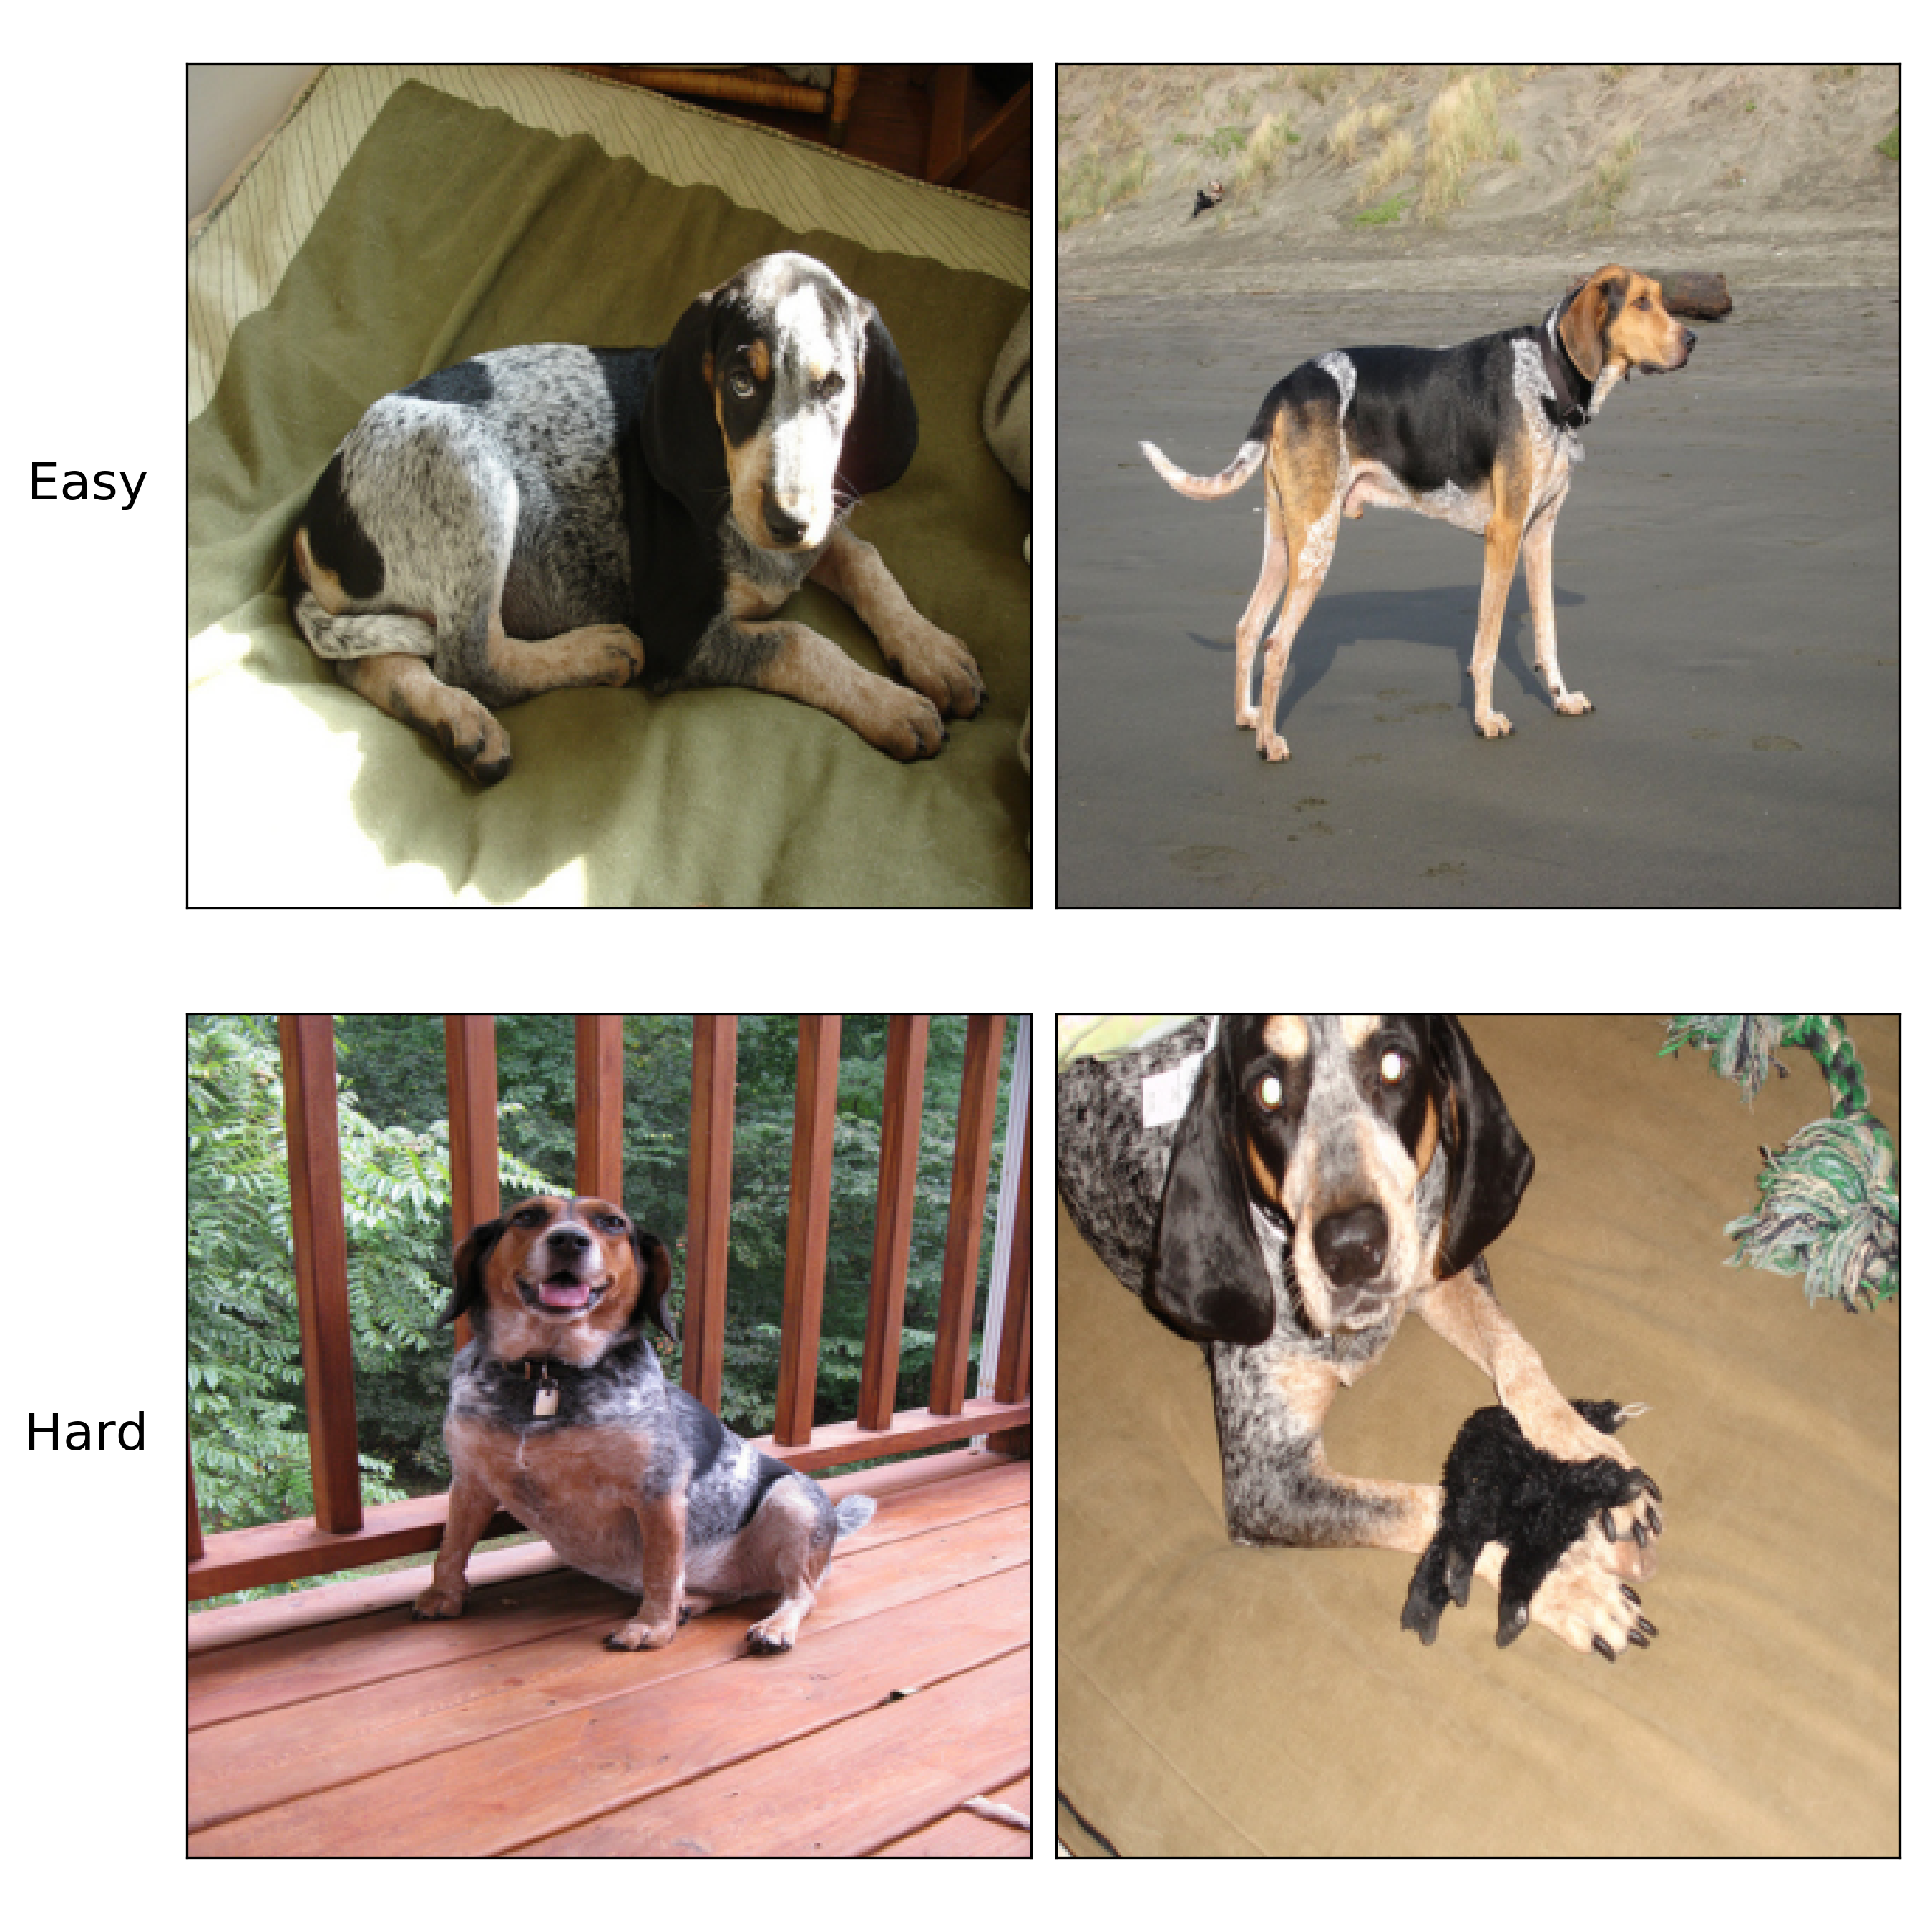
\includegraphics[width=0.45\linewidth]{figures/illustrations/hard_vs_easy_dog}}
	\hfill
	\subfloat[flamingo\label{fig:easyvshardflamingo}]{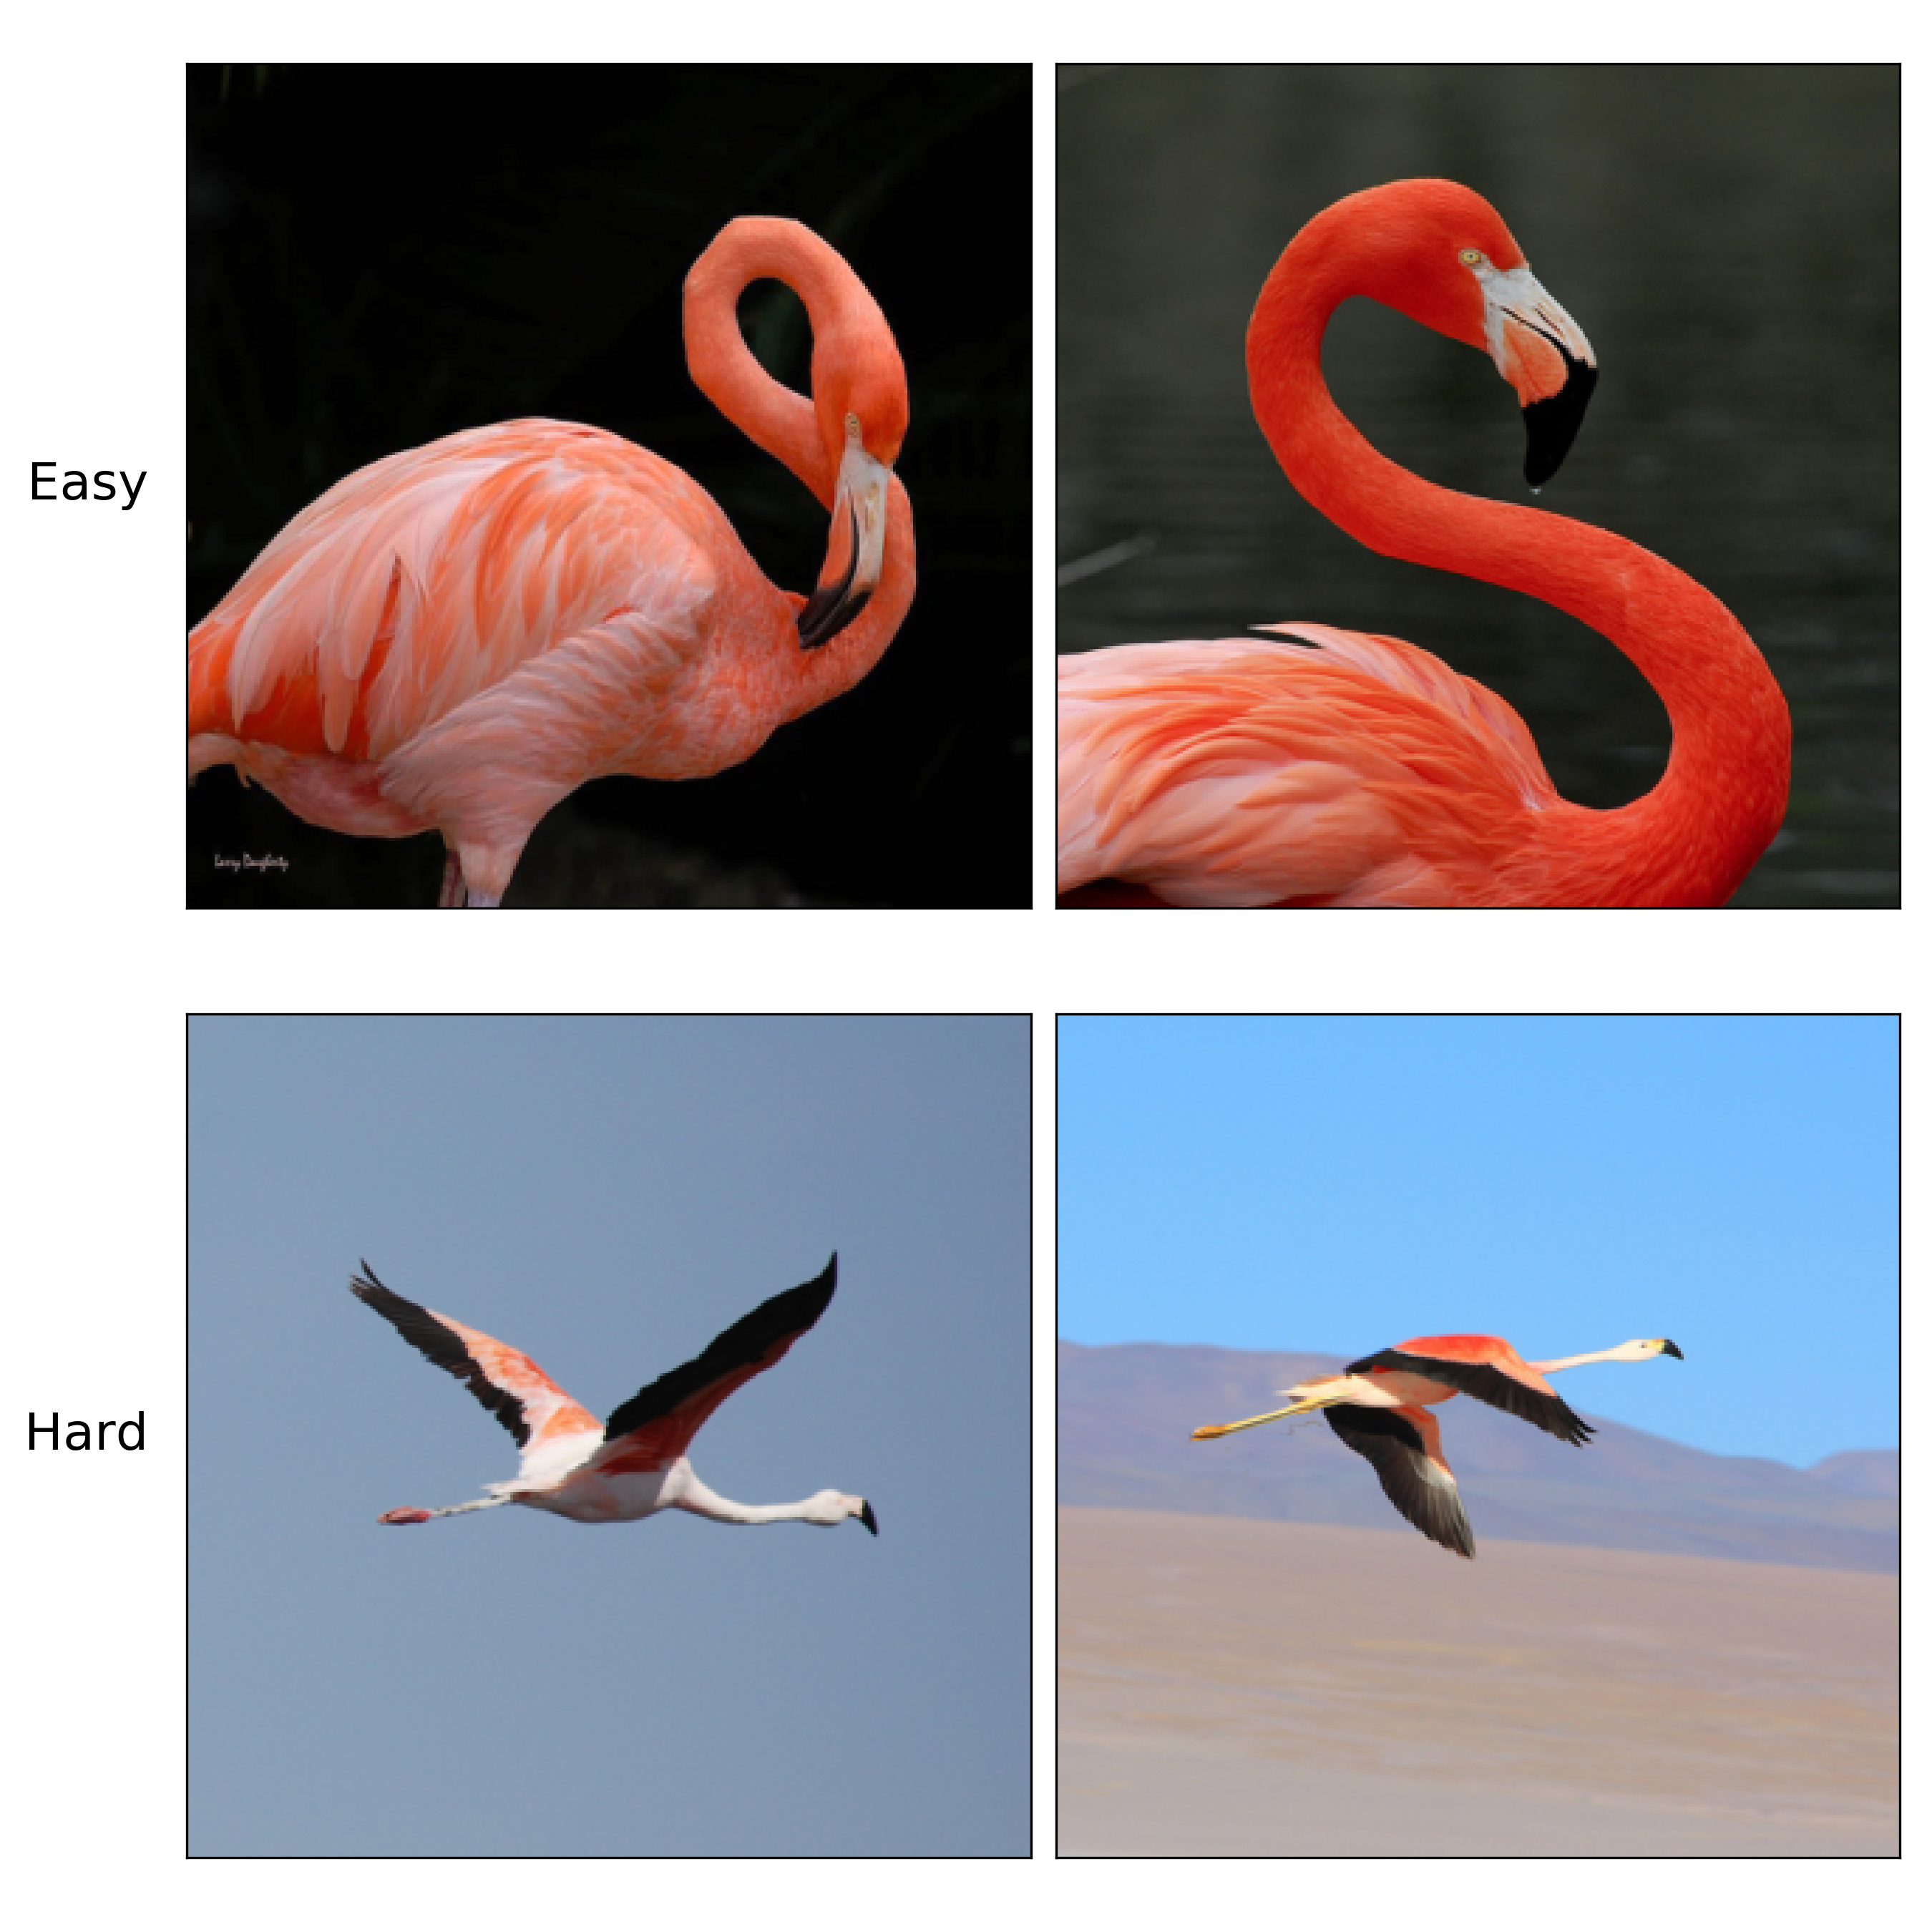
\includegraphics[width=0.45\linewidth]{figures/illustrations/hard_vs_easy_flamingo}}
	\caption[Easy vs. Hard Samples]{Easy vs. Hard Samples: The top row show samples easily classified from the classes and the bottom row show harder samples of the two classes, \protect\subref{fig:easyvsharddog} bluetick and \protect\subref{fig:easyvshardflamingo} flamingo. }
	\label{fig:hardvseasy}
\end{figure}

 These examples have been found by running an early exit model. The hard examples have been found from looking at samples, that the \gls{dnn}s failed to classify, or can only classify using the last exit. The easy example are found by looking at samples, that can be correctly classified with high confidence by the first exit. 
 
 In the next section we present two proposals in literature for early exiting \gls{dnn}.

%Early exiting \gls{dnn} draws inspiration from another \gls{cv} algorithm, Viola-Jones \cite{viola_rapid_2001}. Viola Jones Face Detection was proposed in \citeyear{viola_rapid_2001}. The idea is a stacking or cascaded less accurate predictors to build a strong predictor. The predictors increasingly gain confidence when running the algorithm which termintates when the confidence has reached a threshold. Early exiting \gls{dnn} likewise stacks multiple classifiers. The \gls{dnn} can too be terminated, when a prediction with satisfying confidence is obtained. 



% and have primarily been used to solve two challenges in current literature.
%
%\begin{enumerate}
%	\item Reducing average inference latency and power consumption by letting samples prematurely exit the model based on a threshold measure of confidence \cite{teerapittayanon_branchynet:_2016}.
%	\item Comply with application time constraints by exit selection or sub-model selection. By only inference samples up to a selected exit possible to meet stringent delay constraints and reduce waste of computation \cite{li_edge_2018}. 
%\end{enumerate}

\section{BranchyNet vs. Cascaded DNN} \label{sec:ee-branchy-vs-cascaded}

We describe the two very similar proposals and how they differ. Both \gls{branchynet} \cite{teerapittayanon_branchynet:_2016} and cascaded \gls{dnn} \cite{leroux_resource-constrained_2015} were published around the same time. The cascaded \gls{dnn} adds intermediate classifiers after a layer, or a block of layers in a \gls{dnn}, whereas \gls{branchynet} constructs early exit branches with additional convolution layers, see figure \ref{fig:cascaded-vs-branchy}.

\begin{figure}
	\centering
	\subfloat[Branchy AlexNet, Source \citetitle{teerapittayanon_branchynet:_2016} \cite{teerapittayanon_branchynet:_2016}\label{fig:cascaded-vs-branchy-branchy}]{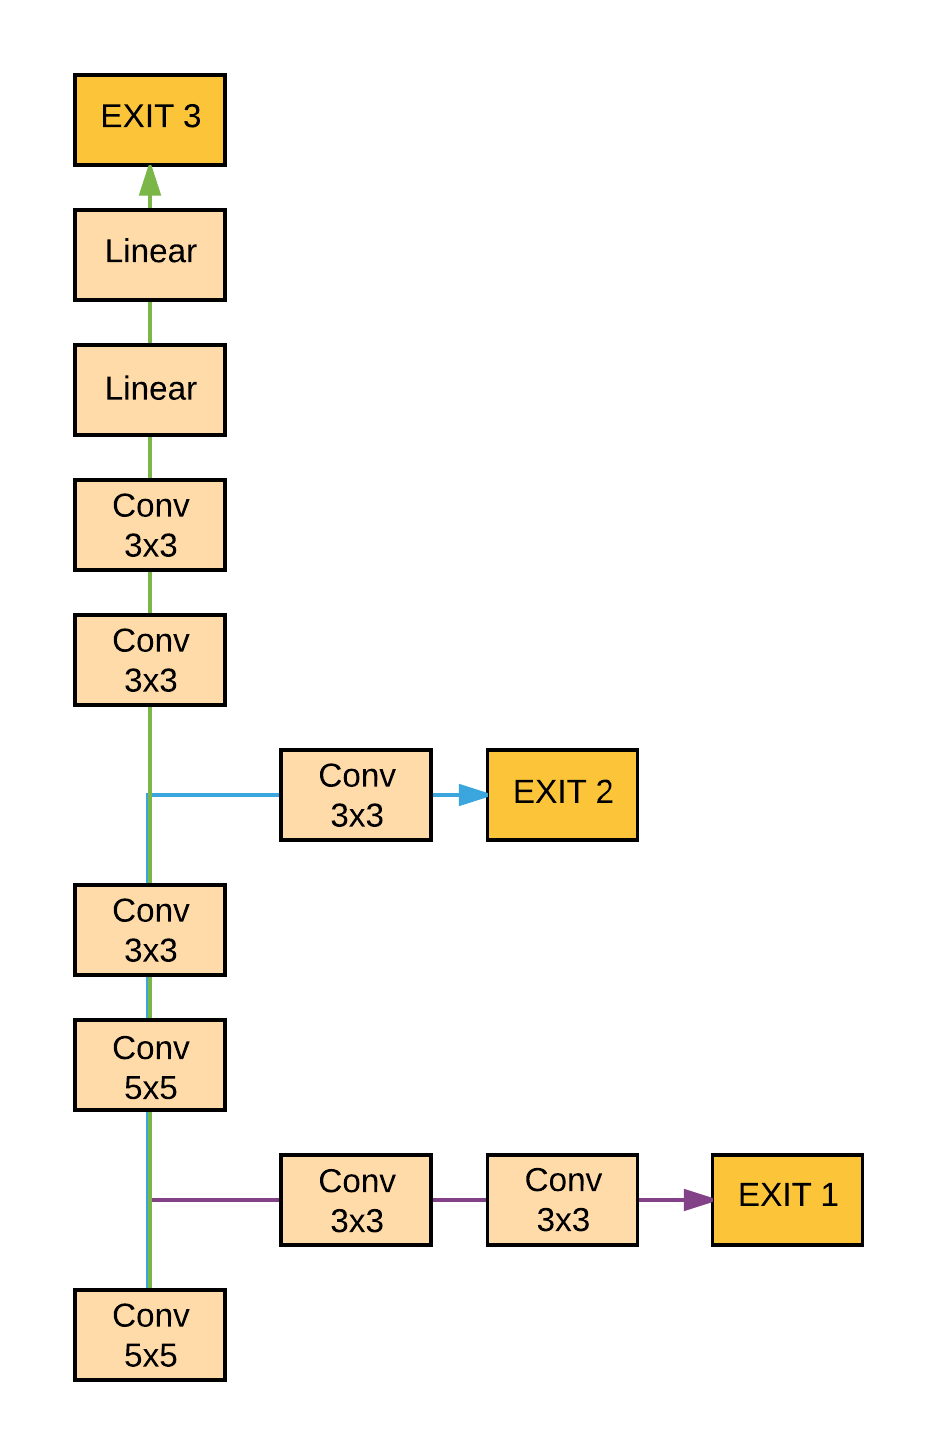
\includegraphics[height=.3\textheight]{figures/articles/branchynet}}
	\hspace{2em}
	\subfloat[Cascaded \gls{dnn}, Source \citetitle{leroux_resource-constrained_2015}\cite{leroux_resource-constrained_2015}\label{fig:cascaded-vs-branchy-cascaded}]{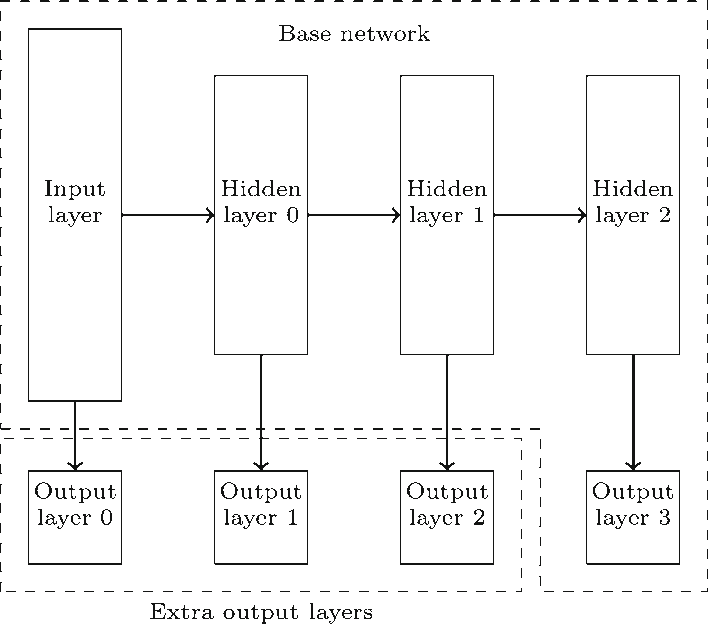
\includegraphics[height=.3\textheight]{figures/articles/cascade_dnn}}
	\caption[\gls{branchynet} vs. Cascaded \gls{dnn}]{\gls{branchynet} vs. Cascaded \gls{dnn}: \protect\subref{fig:cascaded-vs-branchy-branchy} \gls{branchynet} have additional convolution layers in each exit branch, whereas \protect\subref{fig:cascaded-vs-branchy-cascaded} Cascaded \gls{dnn} adds output layers to the layers of the \gls{dnn}.}
	\label{fig:cascaded-vs-branchy}
\end{figure}

Early exiting have shown promising result in other works e.g. \cite{kaya_shallow-deep_nodate, berestizshevsky_sacrificing_2019,panda_conditional_2016}. In \cite{berestizshevsky_sacrificing_2019}, they suggest removing convolutional layers of branches in \gls{branchynet}, to reduce the amount of branch computation. They show a 2 $ \times $ speed-up at only the cost of 1 \% accuracy using two fully-connected layers in exits.
However, in \cite{kaya_shallow-deep_nodate}  a phenomenon named \emph{overthinking} is studied. Overthinking is an early exit correctly classifying an input, but a later exit makes it wrong. To cope with overthinking, they propose not to exit, but make all the exits classify the samples, and use information from all predictions to find the best as the highest scoring prediction. We review the same tendency for our proposed inference scheme, \gls{aee}, in chapter \ref{ch:edgeoffloading}.

\subsection{Fast Inference Framework} 

The inference framework for the two proposal \gls{branchynet} and Cascaded \gls{dnn} are almost identical. A sample is inferred up to an exit, and based on an exit criteria, it is decided to terminate, or to continue to the next exit. 

The algorithm for fast inference using early exit is shown in listing \ref{lst:inference}. 

\begin{minipage}{\linewidth}
	\begin{lstlisting}[language = {}, mathescape=true, caption={Early Exit Fast Inference }, label={lst:inference}]
procedure $\textsc{EarlyExitFastInference}(i, \gamma)$
	for $n = 1\dots N$ do
		$\bm{z} = f_{exit_n}(i)$
		$ \bm{\hat{y}} = softmax(z) $
		if $\max \bm{\hat{y}} > \gamma$ then
			return $\arg \max \bm{\hat{y}}$
	return $\arg \max \bm{\hat{y}}$ 
	\end{lstlisting}
\end{minipage}

Where $ i $ is the input image, $ \bm{z} $ is the output vector from the last linear layer of an exit, and $ \bm{\hat{y}} $ is the output vector from the softmax function. $ N $ is the number of exits and $ \gamma $ is the threshold. The softmax function is defined as
\begin{align}
\bm{\hat{y}} = \frac{e^{z}}{\sum_{j=1}^{C}e^{z_c}}
\end{align}

The only difference between the two proposals are the choice of exit criteria. Cascaded \gls{dnn} uses the softmax score of the prediction, and evaluates if the score higher than a selected threshold, it is exited. \gls{branchynet} determines the entropy $ e $ defined by
\begin{align}
	e = -\sum_{j=1}^{C} y_c \log \hat{y}_c
\end{align}
and evaluates if the entropy is less than a selected threshold. Note listing \ref{lst:inference} uses the softmax output to evaluate against the threshold.

\subsection{Training Framework} 

In \cite{leroux_resource-constrained_2015}, when training cascaded \gls{dnn}, it is proposed to train a network using a single end-classifier. Once the model has reaches convergence, the intermediate classfiers are attached. The entire network is then further trained for one single epoch, before freezing the network weights and training only the classifiers. This is equivalent to use a pre-trained model and convert it to a cascaded model. The approach was tested and gave unsatisfactory results, see figure \ref{fig:frozen-b-resnet-miniimagenet-100}. In \cite{leroux_cascading_2017}, the follow-up paper to cascaded \gls{dnn}, they train a frozen base network on the ImageNet dataset, but does not achieve better performance, than we do using this approach.  

The \gls{branchynet} approach is remarkably similar. In \cite{teerapittayanon_branchynet:_2016} they define the \gls{branchynet} loss function, as an extension of the widely used softmax cross-entropy loss function.
\begin{align}
L\left(\bm{y},\hat{\bm{y}}\right) = - \frac{1}{C} \sum_{j =1}^{C} y_c \log \hat{y}_c
\end{align}
 Where $ \bm{y} $ is a on-hot encoded ground truth vector, $ \bm{\hat{y}} $ is the output score vector of the softmax classfier and $ C $ is the number of classes and $ c \in \left\{1, 2,  \dots, C\right\} $ is the class labels.
	
The \gls{branchynet} loss function is defined as the weighted sum of the softmax cross-entropy loss of each branch-prediction. 
\begin{align}
	L_{\mathrm{BranchyNet}}(\hat{\bm{y}},\bm{y};\theta) = \sum_{n=1}^{N} w_n L \left(\hat{\bm{y}}_{n},\bm{y};\theta\right)
\end{align}
Where $ \bm{\hat{y}}_n $ is the output score vector of exit $ n $, $ w_n $ is the weight for exit $ n $ and $ \theta $ represents the parameters of the layers from an entry point to the exit point $ n $.

They claim, that the joint-optimization of multiple exits provides a regularization effect, thus encountering over-fitting and potentially improves test accuracy. Additionally it also mitigates vanishing gradient, due to additional gradient signal from the early exits, which promotes more discriminative features in early layers. In \gls{googlenet} \cite{szegedy_going_2015} auxiliary classifiers are likewise place in the middle of the network to counter vanishing gradients. However, that is also the only purpose of the auxiliary classifiers, as they are only used when training the network. Thus, no samples can exit the inference process using the auxiliary classifiers. 

In \gls{branchynet}, they have also found, that first training the network end-to-end or using a pre-trained model, and then attach the intermediate exits/classifiers both improves the performance and shortens the training time, as in cascaded \gls{dnn}. However, they do not suggest to freeze the features of the model base. Instead they suggest to train the entire model. We have tried both freezing and unfreezing the network base and have found, that training the entire model is the far superior approach, see figure \ref{fig:b-resnet-miniimagenet-100}. 

In the next section we explain the \gls{msdnet} \cite{huang_multi-scale_2017}, a novel \gls{dnn} specifically designed for early exits.

\section{Multi-Scale Dense Network} \label{sec:ee-msdnet}

\gls{msdnet} \cite{huang_densely_2016} addresses two main problems concerning early exit models. The first problem is the lack of coarse-level features in early classifiers. Traditional \gls{dnn}s uses stacking of layers to get coarse level features, which the early classifier lacks, thus giving unsatisfactory high error-rates for early exits. Multi-scale feature maps addresses this issues by preserving high-resolution information and allow constructing coarse-level features for all classifiers in the network. 

The second problem is early classifiers interfere with later classifiers. The early classifiers might cause early features to be optimized for the short-term by collapsing information prematurely, thus harming the later and final classifiers. Their study reveals, that densely connected layers suffers much less from intermediate classifiers than residual layers, as a layer is connected to all previous layer and is therefore able to recover collapsed information. The residual and densely connected layers are elaboration upon in section \ref{sec:ee-implementation}.


The combination multi-scale feature maps for coarse-level features and information preservation form densely connected layers are shown to be important for early exit models. Figure \ref{fig:msdnet} from the original paper shows the model design. On the vertical axis, are the multi-scale paths, that downscales the input images. On the horizontal axis, are the densely connected layers stacked. Notice, that the concatenation of features (circled c) are done using features from higer scales and from earlier in the same scale-path. Each block of the \gls{msdnet} contains a classifiers, where the model can terminate the inference.
\begin{figure}
	\centering
	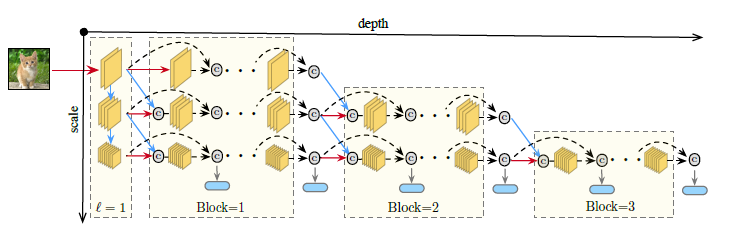
\includegraphics[width=\linewidth]{figures/models/msdnet}
	\caption[\gls{msdnet} Architecture]{\gls{msdnet} Architecture, Source: \citetitle{huang_multi-scale_2017} \cite{huang_multi-scale_2017}}
	\label{fig:msdnet}
\end{figure}
We implement early exiting model using both \gls{resnet} and \gls{densenet} described in section \ref{sec:ee-implementation}. We use our two implemented models and the \gls{msdnet}.
In the next section we describe the mathematical models used to evaluate the latency, accuracy and early exiting capabilities using confidence and delay thresholds.

\newpage\section{Analytical Model} \label{sec:ee-metrics}

In this section we define the analytical model used for our experiments. We compare conventional models with early exiting models. Most \gls{dnn}s are build of blocks of convolution and pooling layers, or at least the ones we use. We adapt the same notation for the early exiting inference model and the conventional inference model with a single exit at the end of the \gls{dnn}, see figure \ref{fig:inference_models}.
	\begin{figure}
		\centering
		\captionsetup[subfigure]{justification=centering, farskip=1pt,captionskip=1pt}
		\subfloat[Conventional Inference Model]{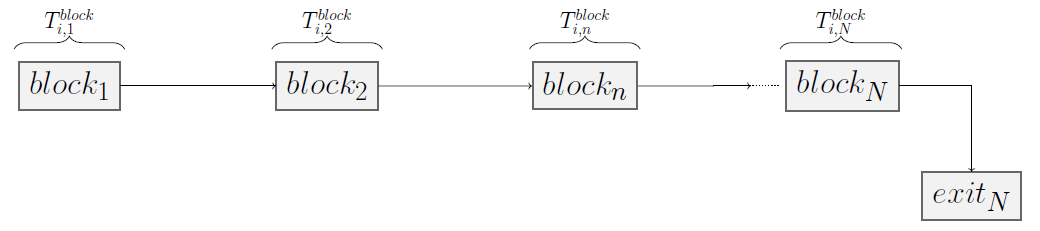
\includegraphics[width=.7\linewidth]{figures/models/conv_math}}
		\hfill
		\subfloat[Early Exit Inference Model]{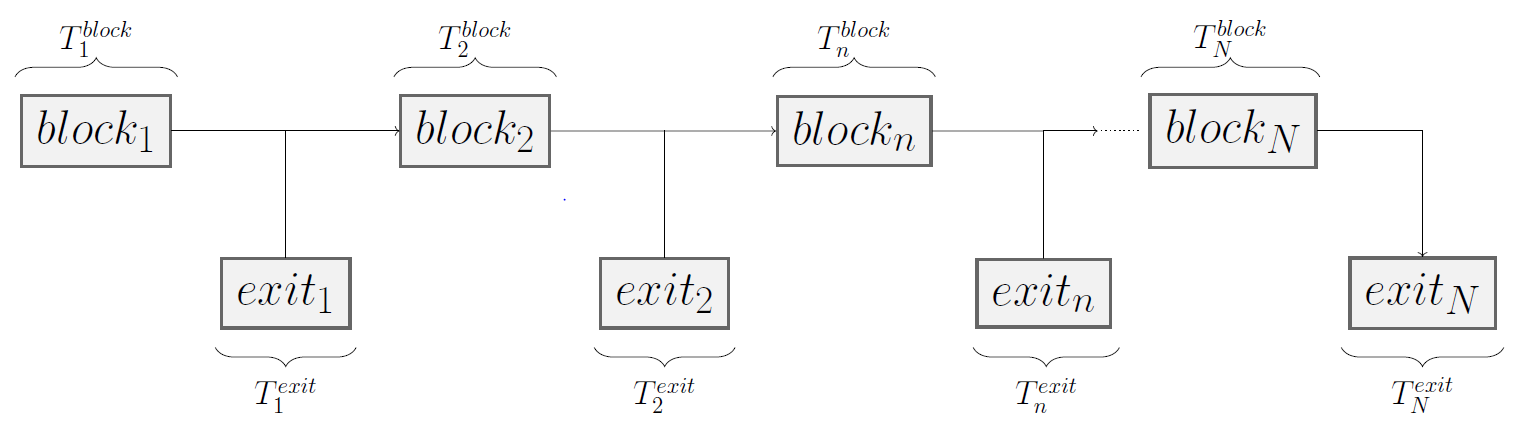
\includegraphics[width=.7\linewidth]{figures/models/exit_math}}
		\caption[\gls{dnn} structure]{\gls{dnn} inference models: A \gls{dnn} is constructed by stacking layers of non-linear function on top of each other to form a \gls{dag}. The layers are typically grouped into blocks, and a classification layer is attached at the end of the network, i.e. exits in our models.}
		\label{fig:inference_models}
	\end{figure}	
	We define the inference latency for both models. We also classification accuracy, early exit condition and our problem formulation. 
	
	Assume $ C $ denotes the number of image classes, $ N $ denotes the number of the exit points in a DNN, $ I $ denotes the number of images.

	\begin{enumdescript}
		\item[Inference Latency] is defined as the response time for a \gls{dnn} to provide a prediction i.e. the time from input to output. 

		Assume:
		\begin{itemize}
			\item $T_{i,n}^{block}$ denotes the runtime of inference an image $ i $ to the $ n $th block of the \gls{dnn} $ i $ for $ \left(1\leq n \leq N, 1 \leq i \leq I\right) $
			\item $T_{i,n}^{exit}$ denotes the runtime of the exit $ n $  to process image $i$ for $ \left(1\leq n \leq N, 1 \leq i \leq I\right) $
		\end{itemize}
		\begin{enumdescript}
			\item[Inference Latency Conventional Model] The conventional inference model only have a single exit at block $ N $, hence all $ N $ blocks of the \gls{dnn} must have inferred the image $ i $ before a classification is reached at exit $ N $. Thus the runtime to classify image $ i $ using a conventional model, is described as
			\begin{align}
			T^{ci}_{i}= \sum_{j=1}^{N} T_{i,n}^{block} + T_{i,N}^{exit}
			\end{align}
			\item[Inference Latency Early Exit Model] The early exit inference model is adaptive. The inference of image $ i $ can terminate at any exit $ n $. If the classification exits from exit point $ n $, then the latency model for early exit inference model is presented as
			\begin{align}
			T_{i,n}^{ee}=\sum_{j=1}^{n} \left(T_{i,n}^{block} + T_{i,n}^{exit} \right) 
			\end{align}
			The additional classifiers of the early exit inference model add a overhead compared to the conventional inference model, however it may not be required to run all $ n $ blocks and classifiers of the early exiting inference model. 
		\end{enumdescript}
		
		\item[Classification Accuracy] is the defined as the fraction of correctly classified samples out of all inferred samples. The inference accuracy can be expressed by
		\begin{align}
		\bar{A}=1-\frac{1}{I} \sum_{i=1}^{I} \mathbb{I}\left(\left|\hat{c}_{i}-c_{i}\right|\right) \label{eq:accuracy}
		\end{align}
		%We can express the ground truth as a one-hot encoded vector $ \bm{y}_i $
		where $ \mathbb{I(\cdot)}  $ is a indicating function defined by
		\begin{align}
		\mathbb{I}(a)= \begin{cases}
		0, & \mathrm{if\:} a \leq 0, \\
		1, & \mathrm{otherwise}
		\end{cases} \label{eq:indicator}
		\end{align}
		and $ c_i \in \left\{1, 2, \dots, C \right\} $ is the ground truth class label of image $ i $,
		
		and $ \hat{c}_i $ is the predicted class for image i $  \hat{c}_i \in \{\hat{c}^*_{i,1} , \hat{c}^*_{i,2}, \dots, \hat{c}^*_{i,N} \} $. 
		
		It means the prediction of either exit point can be used as the output of DNN. Each element $ \hat{c}^*_{i,n} $ in the set denotes the predicted class of exit point $ n $, which is the class with the maximum confident score, i.e.,
		\begin{align}
		\hat{c}^*_{i,n} = \arg \underset{c}{\max}\: \bm{\hat{y}}_{i,n}
		\end{align}
		where $ \bm{\hat{y}}_{1,n} $ is the confidence score vector output from the softmax classifier of exit point $ n $, i.e.,
		\begin{align}
		\bm{\hat{y}}_{i,n} = \left[\begin{array}{ccccc}\hat{y}_{i,n,1} & \hat{y}_{i,n,2} & \hat{y}_{i,n,c} & \dots & \hat{y}_{i,n,C}\end{array}\right]
		\end{align}
		Each element $ \hat{y}_{i,n,c} \in \bm{\hat{y}}_{i,n} $ represents the score of class $ c $ from exit point $ n $ by processing image $ i $.
		
		Note the accuracy for each individual exit can be described as
		\begin{align}
		\bar{A}_n=1-\frac{1}{I} \sum_{i=1}^{I} \mathbb{I}\left(\left|\hat{c}^*_{i,n}-c_{i}\right|\right)
		\end{align}
  
		\item[Early Exit Condition] we define the early exit condition based on the output of our scoring function $ f_\phi(\bm{\hat{y}}_{i,n}) $, given the score vector $ \bm{\hat{y}}_{i,n} $ for image $ i $ at exit point $ n $. An image $ i $ is allowed to exit the model at exit point $ n $, if a score threshold $ \gamma $ is surpassed. 
		
		We assume $	\gamma \in \left[0,1\right] $, as the all scores of  $ \bm{\hat{y}}_{i,n} $ sum to 1. Note that, although the score threshold could be different for each exit point, in our experiments, we use the same threshold, since we are concerned with the latency. Selecting a higher threshold value at an early exit, will cause less samples to exit and promote the use of later exits, which will cause additional inference delay. It is seen in \cite{teerapittayanon_finding_2018}, that finding different threshold values for the exits can improve the accuracy.
		
		We express the probability of early exit at exit $ n $, given the score function. 
		\begin{align}
		\overline{F}^{exit}_n = \frac{1}{I}\sum_{i=1}^{I} \mathbb{I} \left(\gamma-f_{\phi}\left(\bm{\hat{y}}_{i,n}\right) \right)
		\end{align}
		Where $ f_\phi\left(\bm{\hat{y}}_{i,n}\right) $ is a scoring function and for notation simplicity we write 
		\begin{align}
			f_{\phi}\left(\bm{\hat{y}}_{i,n}\right) = \begin{cases}
			 	f_{max}\left(\bm{\hat{y}}_{i,n}\right)\\
			 	f_{margin}\left(\bm{\hat{y}}_{i,n}\right)
			\end{cases}
		\end{align}
		which means we can choose to use either one. Next We define two different score functions.
		
		\begin{enumdescript}
			\item[Score-Max] the score-max function $ f_{max}(\cdot)$ also used in \cite{leroux_resource-constrained_2015}, is a simple function, that takes the score vector $ \bm{\hat{y}}_{i,n} $ of image $ i $ at exit $ n $ as input and outputs the maximum value of the vector. We express it as 
			\begin{align}
			f_{max}\left(\bm{\hat{y}}_{i,n}\right) = \underset{c}{\max} \bm{\hat{y}}_{i,n}
			\end{align}
			\item[Score-Margin] the score-margin function $ f_{margin}(\cdot)$, is defined and used in \cite{park_big/little_2015}. The function also takes the $ \bm{\hat{y}}_{i,n} $ as input and returns the difference between the two largest elements. We express it as
			\begin{align}
			f_{margin}\left(\bm{\hat{y}}_{i,n}\right) = \hat{y}_{i,n}^{1st} - \hat{y}_{i,n}^{2nd} \label{eq:f_margin}
			\end{align}
			where $ \hat{y}_{i,k}^{1st} $ denotes the largest element of $ \bm{\hat{y}}_{i,n} $ 
			and $ \hat{y}_{i,n}^{2nd} $ the second largest element of $ \bm{\hat{y}}_{i,n} $.
			
		\end{enumdescript}
	
	\item[Reliability] the reliability is defined as the accuracy we can obtain given a deadline $ \delta $. Our main concern is time-critical application.
	
	\begin{align}
	R= \bar{A} \cdot (1-\overline{F}^{to})
	\end{align}
	
	The deadline we formulate as the timeout probability $ \overline{F}^{to} $- It is defined as the number of samples not able to meet the deadline out of all samples in the set.
	\begin{align}
	\overline{F}^{to}=\frac{1}{I}\sum_{i=1}^{I} \mathbb{I}\left(T_{i}^{cmp}-\delta\right)
	\end{align}
	Where $ T_{i}^{cmp} $ denotes the runtime to process image i. We can choose a conventional model or an early exit model 
	\begin{align}
		T^{cmp}_i = \begin{cases}
			T^{ci}_i \\
			T^{ee}_i
		\end{cases}
	\end{align}
	We only have a delay violation if $ T_i^{cmp} \leq \delta $, i.e. the model have not provided a single prediction within the time frame. Thus, if no exit of the model can meet the delay requirements and a prediction cannot be acquired, it is treated as a misclassification. 
		
	\item[Problem formulation] We want to maximize the reliability for each image by selecting the best possible exit
	\begin{maxi}
		{\vec{n}}{R}
		{}{}
	\end{maxi}
	where $ \vec{n} = \left\{ n_1, n_2, \dots, n_I \right\}$ is a vector to denote which exit point would be used for prediction image $ i $ for available exit point $ n_i \in \left\{1,2, \dots, N\right\} $.
	
	To solve this problem, instead of making decision before processing the image, we simply use a best effort way, i.e., feed each exit results back and let user decide the prediction. For three reasons:
	\begin{enumerate}
		\item latency uncertainty make it hard to make decision in advance
		\item algorithm to make decision may take time
		\item going through classifier of each exit point would not take too long time.
	\end{enumerate}
		
	\end{enumdescript}

\section{Implementation} \label{sec:ee-implementation}

In this section we describe our implementation of early exit models. We have implemented \gls{bresnet} and \gls{bdensenet}.  

\subsection{Branchy-ResNet} 

In this section is the residual layer explained. The residual layer is the building block of the residual networks. Furthermore we describe the implementation of \gls{bresnet}.

Residual Networks or \gls{resnet} \cite{he_deep_2015} have for long been a state-of-the-art network and won ILSVRC15 using 152 layers. The network is build of residual blocks, a \gls{dnn} layer designed for extremely deep networks. 

Just as plain \gls{vgg} networks \cite{simonyan_very_2015}, residual networks is still a stacking of convolution layers. The depth of \gls{dnn}s is of paramount importance to extract increasingly richer features from images to obtain highly accurate classification models. Training very deep models with more than ten layers to convergence is not easy due to vanishing/exploding gradients. The \gls{resnet} adds a shortcut connection, which skips a layer or a block of layers. The skip connection adds the identity of the input to the output of the layer or block, see figure \ref{fig:residualblock}

\begin{figure}
	\centering
	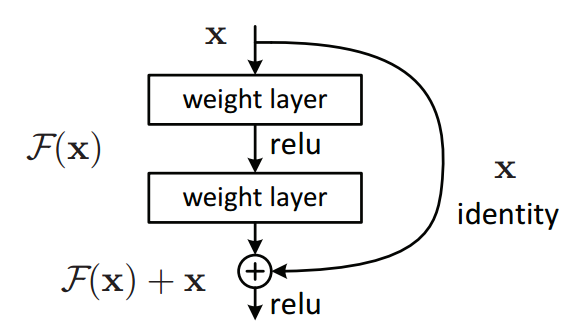
\includegraphics[width=.5\linewidth]{figures/models/residualblock}
	\caption[Residual Block]{Residaul Block: A residual block adds the identity i.e. the input to the layer or block of layers to the ouput of the block. Source: \citetitle{he_deep_2015} \cite{he_deep_2015}}
	\label{fig:residualblock}
\end{figure}

Information from earlier layers are preserved by the skip connection, which diminishes the vanishing gradient problem. Thus this type of network have shown to be easier to train compared to it’s plain counterpart, and able to obtain far superior accuracy.  

Very deep residual networks comprised of up to 152 layers have also shown to be far more efficient, requiring less \gls{flop}s, than \gls{vgg}16 comprised of only 16 layers, by introducing a bottleneck unit.

The residual networks proposed in \cite{he_deep_2015} are grouped into 4 resolutions block each of which downsamples the input data. The network are proposed with different number of layers $ \left\{18, 34, 50, 101, 152\right\} $ exemplifying the ability to train extremely deep networks. Table \ref{tbl:resnet101} describes the blocks and layers of the \gls{resnet} architecture. \gls{pytorch} provide implementations of these networks. The implementations can be trained from scratch or can be initialized with downloadable pretrained weights based on ImageNet. \gls{resnet}101 have been chosen for this project, as it has comparable depth to the smallest available \gls{pytorch} \gls{densenet}-121 implementation and also have similar inference latency on a Titan Xp (8.90ms and 8.93ms) \cite{bianco_benchmark_2018}.

\small
\begin{center}

\begin{minipage}[c]{\linewidth}
\begin{longtabu}{>{\bfseries}X|X[c]|X[2c]}
	\caption[\gls{resnet}101 description]{\gls{resnet}101 description. The table describes the blocks of \gls{resnet}101, the size of the block and the layers of the block. Note, a pooling layer is placed at the end of each resolution block to downsample the data size.} \label{tbl:resnet101} \\
	\toprule
	\rowfont{\bfseries}
	Resolution block & Output size & Layer description \tabularnewline
	\hline
	\endfirsthead
	\multicolumn{3}{@{}l}{\textbf{\textcolor{black}{Table \ref{tbl:resnet50}:}} continued}\\
	\toprule
	\rowfont{\bfseries}
	Conv block & Output size & Layer description \tabularnewline
	\hline
	\endhead % all the lines above this will be repeated on every page
	\hline
	\multicolumn{3}{@{}l}{continued \ldots}\\
	\endfoot
	\hline
	\endlastfoot
	conv1 & $112\times 112$& $7\times 7, 64, \:\mathrm{stride}\: 2$ \tabularnewline \hline
	
	\multirow{5}{*}{conv2\_x} 	& \multirow{5}{*}{$56 \times 56$} 	& $3 \times 3 \:\mathrm{maxpool, stride}\: 2 $ \\ \tabucline{3-3} & & \multirow{4}{*}{
		$\begin{bmatrix}
		1 \times 1, 64 \\ 3 \times 3, 64 \\1 \times 1, 256
		\end{bmatrix} \times 3$ }		\tabularnewline										
	& & 	\tabularnewline
	& & 	\tabularnewline
	& & 	\tabularnewline
	\hline
	
	\multirow{4}{*}{conv3\_x} 	& \multirow{4}{*}{$28\times 28$} & \multirow{4}{*}{
		$\begin{bmatrix}
		1 \times 1, 128 \\ 3 \times 3, 128 \\1 \times 1, 512
		\end{bmatrix} \times 4$ }		\tabularnewline										
	& & 	\tabularnewline
	& & 	\tabularnewline
	& & 	\tabularnewline
	\hline
	
	\multirow{4}{*}{conv4\_x} 	& \multirow{4}{*}{$14\times 14$} & \multirow{4}{*}{
		$\begin{bmatrix}
		1 \times 1, 256 \\ 3 \times 3, 256 \\1 \times 1, 1024
		\end{bmatrix} \times 23$}		\tabularnewline										
	& & 	\tabularnewline
	& & 	\tabularnewline
	& & 	\tabularnewline
	\hline
	
	\multirow{4}{*}{conv5\_x} 	& \multirow{4}{*}{$7\times 7$} & \multirow{4}{*}{
		$\begin{bmatrix}
		1 \times 1, 512 \\ 3 \times 3, 512 \\1 \times 1, 2048
		\end{bmatrix} \times 3$}		\tabularnewline										
	& & 	\tabularnewline
	& & 	\tabularnewline
	& & 	\tabularnewline
	\hline
	
	Classifier & \multicolumn2{c}{$\mathrm{Avg.\: Pool,\:} 1000d\: \mathrm{fc,\: Softmax}$} \tabularnewline
	\bottomrule
\end{longtabu}
\color{caption-color}{\textit{Source: \citetitle{he_deep_2015}, by \citeauthor{he_deep_2015} \cite{he_deep_2015}, describes a full list of Residual Networks (\gls{resnet}18, \gls{resnet}34, \gls{resnet}50, \gls{resnet}101 and \gls{resnet}152)}}\color{main-color}
\end{minipage}
\end{center}
\normalsize

The early exits of \gls{bresnet} is placed immediately after a resolution block, as;
\begin{enumerate}
	\item The exit must be placed sufficiently deep, so that the model is actually able to correctly predict some input samples
	\item If used in a collaborative setup, a smaller feature representation is desired to reduce the offloaded data size. The exits are placed after the resolution block, as the filter size is unchanged within the block. 
\end{enumerate}
To contruct the early exits a pooling-layer followed by a fully-connected linear with the softmax classifier is added. Figure \ref{fig:b-resnet} illustrates the early exiting model \gls{bresnet}.

\begin{figure}
	\centering
	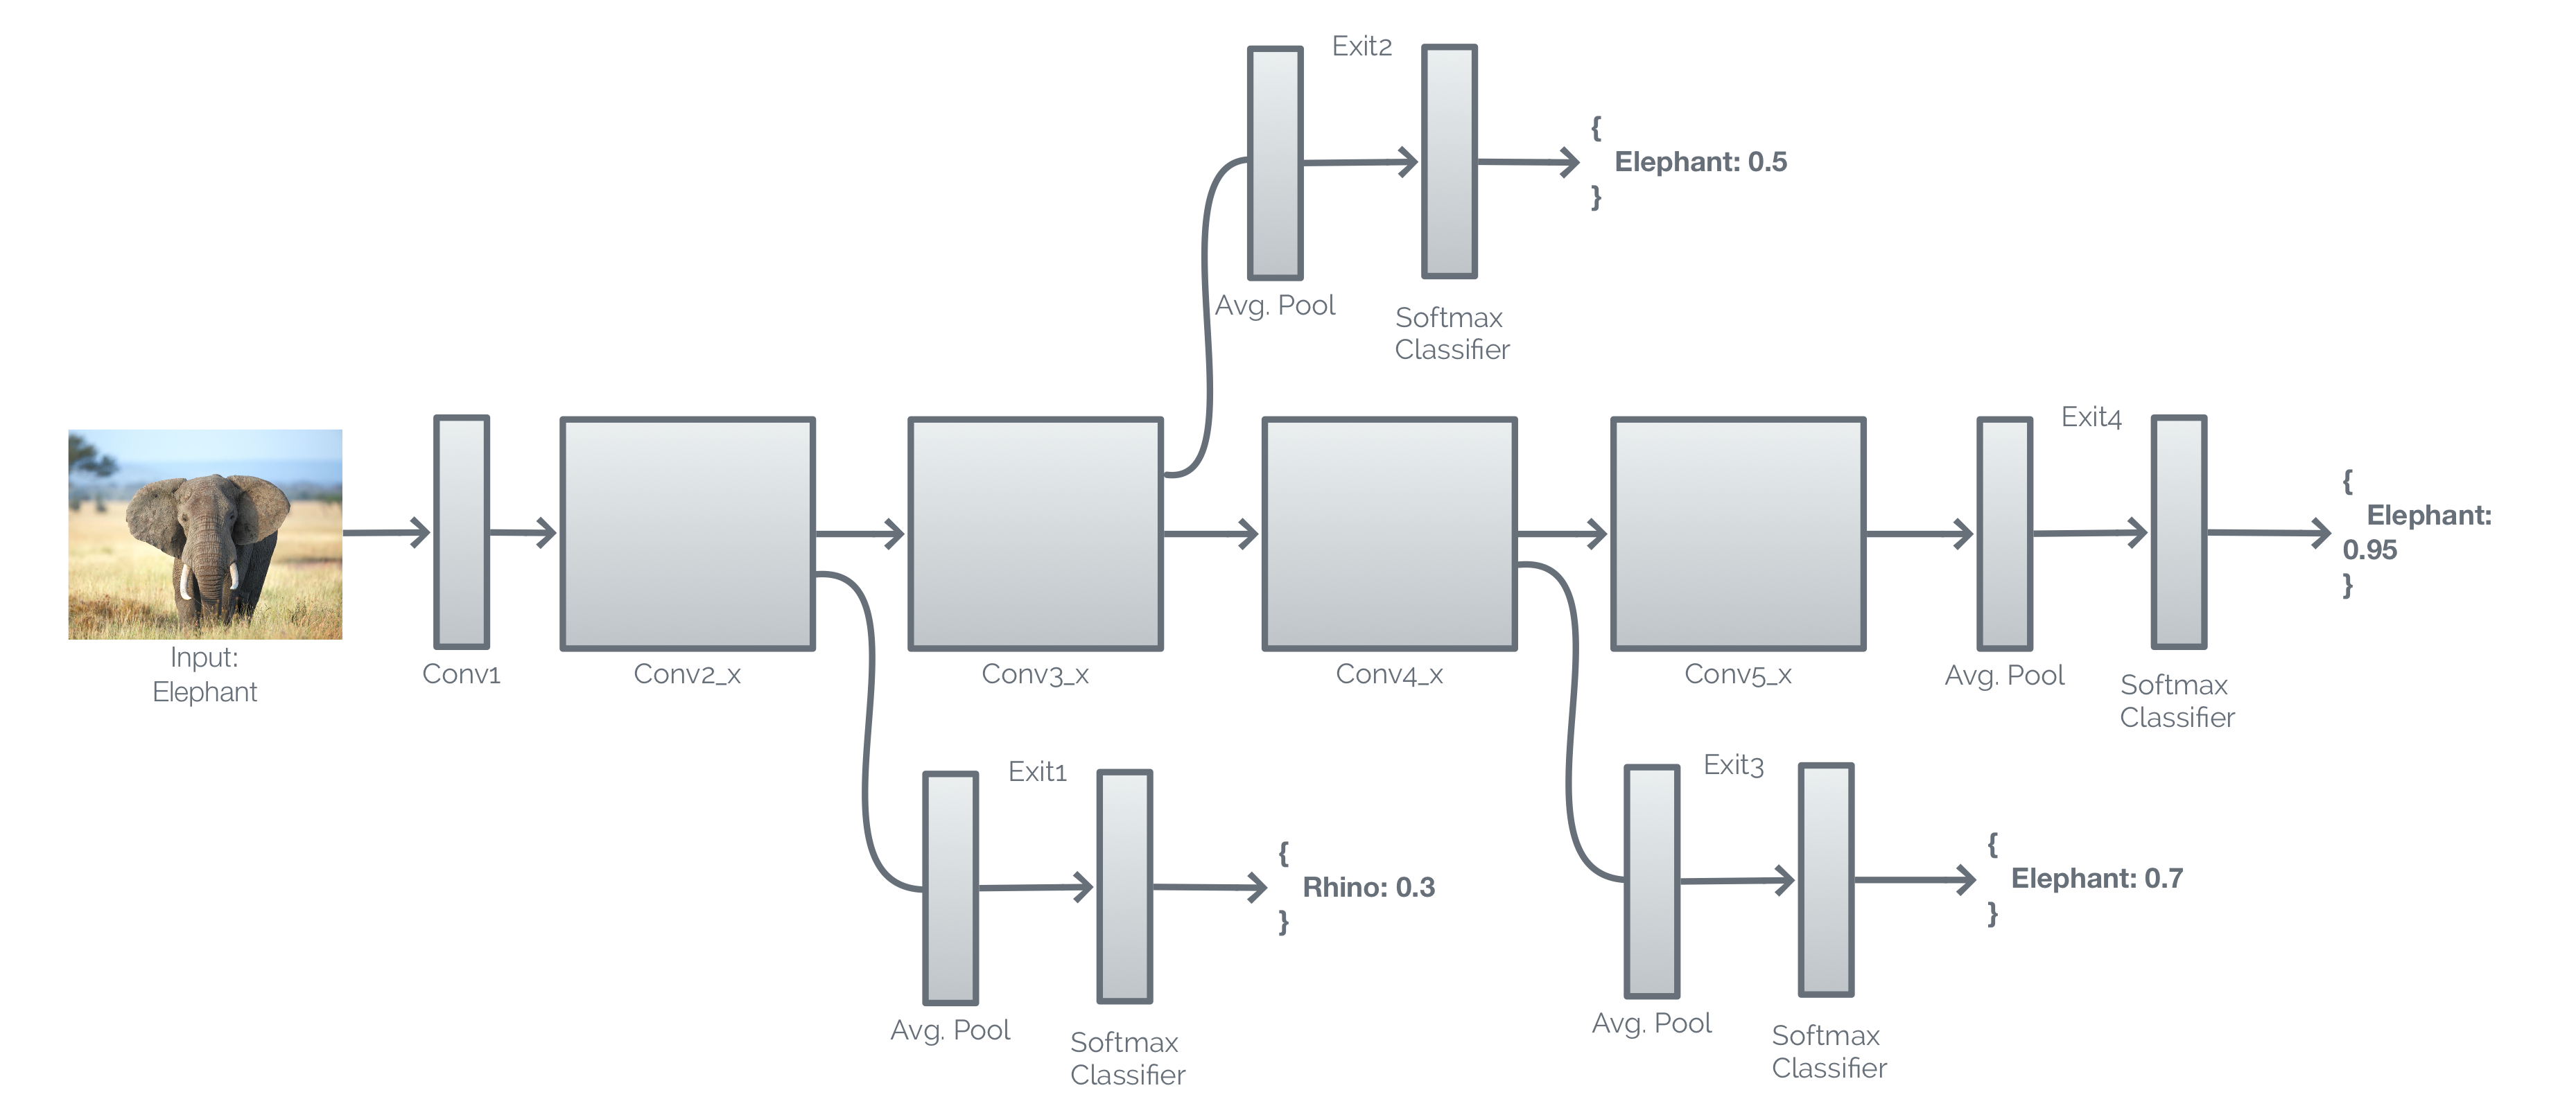
\includegraphics[width=\linewidth]{figures/models/BResNet}
	\caption[B-\gls{resnet} architecture]{\gls{bresnet}: extendeding the \gls{resnet}101 to implement the BranchyNet framework. The figure illustrates how classification confidence grows, as we go deeper in the model. Note, The first exit actually fails to classify the elephant. }
	\label{fig:b-resnet}
\end{figure}

\newpage\subsection{Branchy-DenseNet}

In this section is the dense layer, the building block of the densely connected networks, explained. Followed by a design description of \gls{bdensenet}.

DenseNet \cite{huang_densely_2016} is build on the assumption, that many layers of a \gls{resnet} only have a small contribution to the output and can in fact be dropped during training \cite{huang_densely_2016}. Instead of adding previously learned information to the output, \gls{densenet} combines features from all subsequent layers by concatenation, as there is no need to relearn redundant information. Figure \ref{fig:densenet} show the dense connections, that combine features from all subsequent layers in a block. The feature size grows throughout a densely connected block, as a result of the concatenation. Thus, \gls{densenet} can be thinner as the number of channel can be fewer, which makes it more efficient compared to traditional and residual networks. Additionally densely connected blocks have a regularizing effect, thus reducing overfitting and have shown to train better on smaller data sets.

\begin{figure}
	\centering
	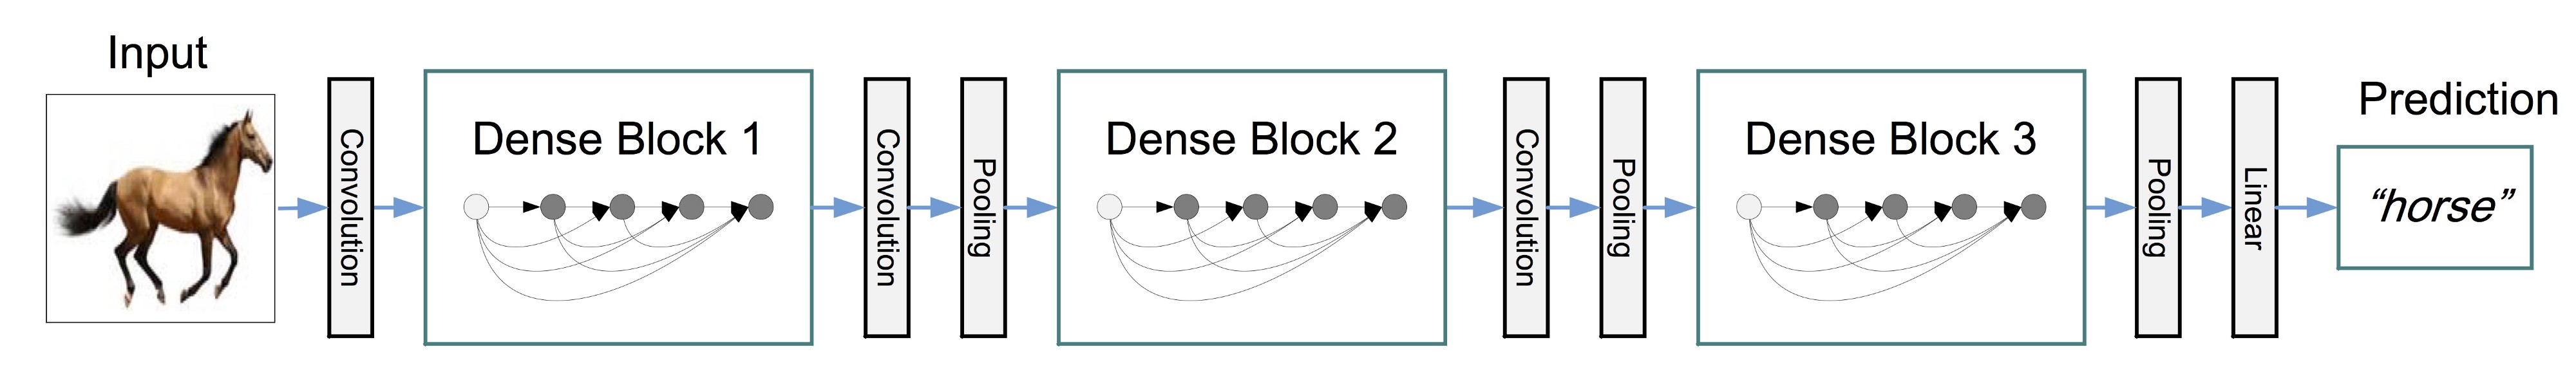
\includegraphics[width=\linewidth]{figures/models/densenet}
	\caption[\gls{densenet}]{\gls{densenet}: The densely connected layers are similarly to residual network grouped into blocks called dense blocks, but for \gls{densenet} intermediate transition layers, consisting of both a convolution and pooling layer, are added between dense block to downsample the feature size. Source: \citetitle{huang_densely_2016} \cite{huang_densely_2016}.}
	\label{fig:densenet}
\end{figure}

Table \ref{tbl:densenet121} describes the block and layers of the \gls{densenet} architecture. 

In \cite{huang_multi-scale_2017}, they argue, that the collective knowledge from all preceding layers of \gls{densenet} gives more diversified features compared to the correlated features of \gls{resnet}s. In \cite{huang_multi-scale_2017} the diversified features are shown to be more suited for early exiting, as the information are better preserved using dense connection. Additionally they show, the placement of an intermediate classifier have less impact on the learned features for a later classifier, as information collapsed to generate a short-term feature for the classifier, are restored by the dense connections.


\begin{small}
\begin{minipage}[c]{\linewidth}
\begin{longtabu}{>{\bfseries}X|X[c]|X[2c]}
	\caption[\gls{densenet}-121 description]{\gls{densenet}-121 description. The table describes the blocks of \gls{densenet}-121. $k$ is the growth rate of the DenseBlock. A typical setting is $k=32$ yielding 256, 512 and 1024 output channels for denseblock(1-3) respectively. The transition layer downsamples the output channel by a factor of 2, thus the number of input channels for DenseBlock(2-4) becomes 128, 256 and 512 respectively.} \label{tbl:densenet121} \\
	\toprule
	\rowfont{\bfseries}
	Layers & Output size & Layer description \tabularnewline
	\hline
	\endfirsthead
	\multicolumn{3}{@{}l}{\textbf{\textcolor{black}{Table \ref{tbl:resnet50}:}} continued}\\
	\toprule
	\rowfont{\bfseries}
	Layers & Output size & Layer description \tabularnewline
	\hline
	\endhead % all the lines above this will be repeated on every page
	\hline
	\multicolumn{3}{@{}l}{continued \ldots}\\
	\endfoot
	\hline
	\endlastfoot
	Convolution & $112\times 112$& $7\times 7, \:\mathrm{stride}\: 2$ \tabularnewline \hline
	Pooling & $56\times 56$& $3\times 3, \:\mathrm{maxpool},\:  \mathrm{stride}\: 2$ \tabularnewline \hline
	\multirow{3}{*}{DenseBlock (1)} 	& \multirow{3}{*}{$56 \times 56$} & \multirow{3}{*}{
		$\begin{bmatrix}
		1 \times 1, k \\ 3 \times 3, k \\
		\end{bmatrix} \times 6$ }		\tabularnewline										
	& &  	\tabularnewline
	& & 	\tabularnewline
	\hline
	
	Transition  	& $56 \times 56$ & $1 \times 1\: \mathrm{conv}$ \tabularnewline \tabucline{2-3}							
	Layer (1) & $28\times 28$ & $2\times 2\: \mathrm{average\: pool,\: stride}\: 2$	\tabularnewline
	
	\hline
	
	\multirow{3}{*}{DenseBlock (2)} 	& \multirow{3}{*}{$28 \times 28$} & \multirow{3}{*}{
		$\begin{bmatrix}
		1 \times 1, k \\ 3 \times 3, k \\
		\end{bmatrix} \times 12$ }		\tabularnewline										
	& &  	\tabularnewline
	& & 	\tabularnewline
	\hline
	
	Transition  	& $28 \times 28$ & $1 \times 1\: \mathrm{conv}$ \tabularnewline \tabucline{2-3}							
	Layer (2) & $14\times 14$ & $2\times 2\: \mathrm{average\: pool,\: stride}\: 2$	\tabularnewline
	
	\hline
	
	\multirow{3}{*}{DenseBlock (3)} 	& \multirow{3}{*}{$14 \times 14$} & \multirow{3}{*}{
		$\begin{bmatrix}
		1 \times 1, k \\ 3 \times 3, k \\
		\end{bmatrix} \times 24$ }		\tabularnewline										
	& &  	\tabularnewline
	& & 	\tabularnewline
	\hline
	
	Transition  	& $14 \times 14$ & $1 \times 1\: \mathrm{conv}$ \tabularnewline \tabucline{2-3}							
	Layer (3) & $7\times 7$ & $2\times 2\: \mathrm{average\: pool,\: stride}\: 2$	\tabularnewline
	
	\hline
	
	\multirow{3}{*}{DenseBlock (4)} 	& \multirow{3}{*}{$7 \times 7$} & \multirow{3}{*}{
		$\begin{bmatrix}
		1 \times 1, k \\ 3 \times 3, k \\
		\end{bmatrix} \times 16$ }		\tabularnewline										
	& &  	\tabularnewline
	& & 	\tabularnewline
	\hline
	
	Classification  	& $1 \times 1$ & $7 \times 7\: \mathrm{global\: average\: pool}$ \tabularnewline \tabucline{2-3}							
	Layer &  \multicolumn2{c}{$\mathrm{Avg.\: Pool,\:} 1000d\: \mathrm{fc,\: Softmax}$} \tabularnewline
	\bottomrule
\end{longtabu}
\color{caption-color}{\textit{Source: \citetitle{huang_densely_2016}, by \citeauthor{huang_densely_2016} \cite{huang_densely_2016}, describes a full list of Densely Connected Networks (\gls{densenet}-121, \gls{densenet}-169, \gls{densenet}-201 and \gls{densenet}-264)}} \color{main-color}
\end{minipage}
\end{small}


For the \gls{bresnet}'s,  we choose to place the exits after the densely connected blocks, for two reasons: 
\begin{enumerate}
	\item We must to go sufficiently deep to obtain features that can correctly classify some samples.
	\item We place exits before the transition layer to avoid unnecessary downsampling if exiting is already possible. 
\end{enumerate}

Note, partitioning for remote execution is done after the transition layer, as a smaller data size can be offloaded. Figure \ref{fig:b-densenet} illustrates the exit placement.

\begin{figure}
	\centering
	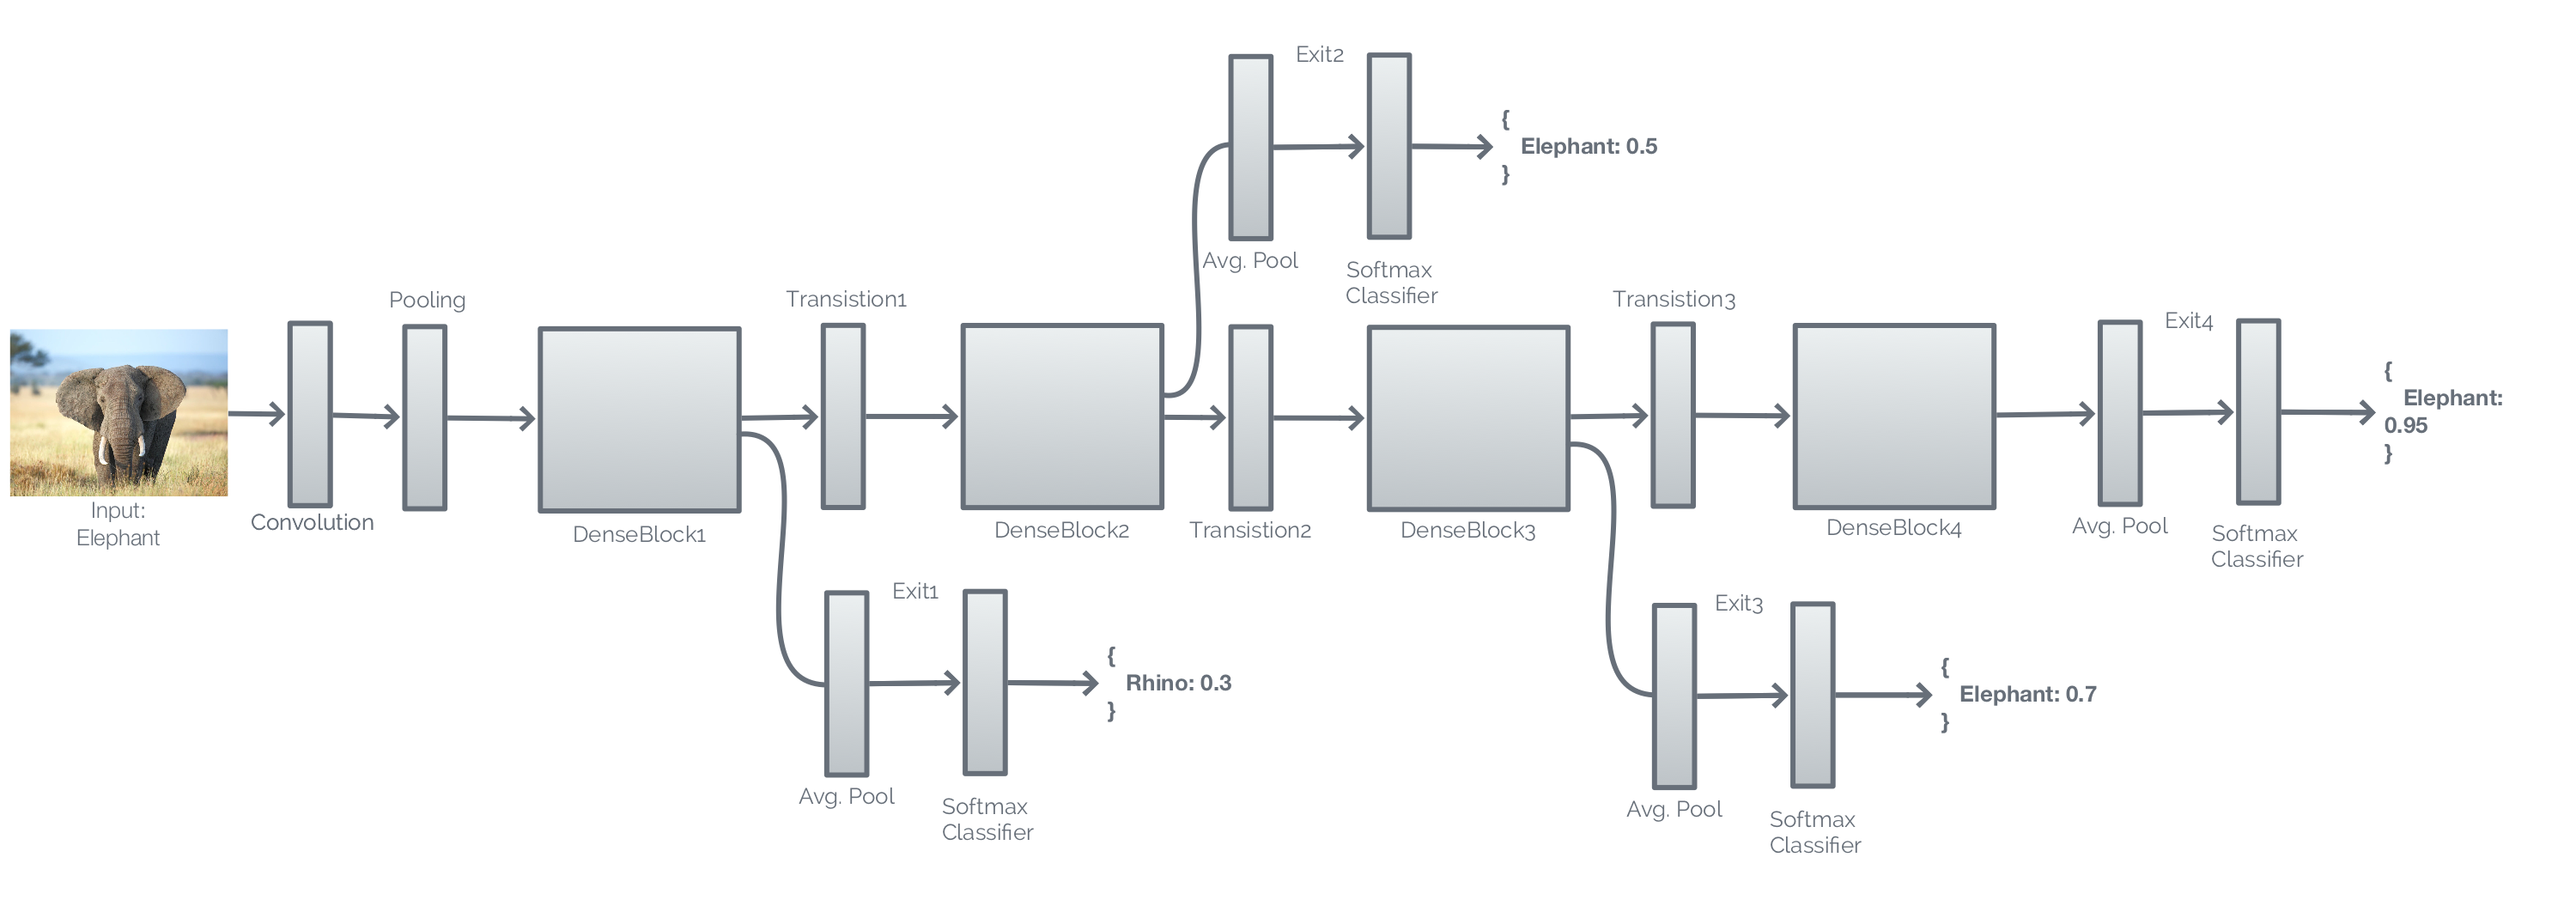
\includegraphics[width=\linewidth]{figures/models/b-densenet}
	\caption[B-\gls{densenet} architecture]{\gls{bdensenet}: \gls{densenet}-121 extended to implement the \gls{branchynet} framework. The figure illustrates the placement of exits after a densely connected block. If the sample could not be exited the inference continues to the transition layer, that downsample the input for the next dense block. }
	\label{fig:b-densenet}
\end{figure}

\section{Experimental Setup} \label{sec:ee-exp-setup}

All code is written in \gls{python} 3.7 \cite{van_rossum_python_1995} using the \gls{pytorch} 1.2
framework \cite{paszke_automatic_2017} and using the \gls{torchvision} 0.4 library \cite{marcel_torchvision_2010}. All code is available at:
{\color{sns-grey}\url{https://github.com/AlexKarlsen/thesis-src}}. 

Table \ref{tbl:platforms} lists the hardware platforms used for the experiments, and its characteristics. Table \ref{tbl:models} lists the models used in the experiment and compares the number of layers, parameters and \gls{flop}s of the models. The number of parameters and \gls{flop}s have been found using \gls{thop} \cite{zhu_thop_nodate}, by inference a random 4d tensor of size $ (\mathrm{batch,channels,width,height})=(1,3,224,224) $ to all models.
 
 \begin{minipage}[t]{\linewidth}
\todo{why those platforms?}
\begin{longtabu}{>{\bfseries}X[0.8]|X[0.8]|X[1.5]|X[r0.3]}
	\caption[Platform hardware comparison]{Platform hardware comparison of Window 10 Stationary PC named \gls{gpu-ws}, a NVIDIA \gls{jetson} development edge computer, and an Intel \gls{nuc} mini pc} \label{tbl:platforms} \\
	\toprule
	\rowfont{\bfseries}
	Platform & CPU & GPU & RAM  \tabularnewline
	\bottomrule
	\endfirsthead
	\multicolumn{3}{@{}l}{\textbf{\textcolor{black}{Table \ref{tbl:platforms}:}} continued}\\
	\toprule
	\rowfont{\bfseries}
	Platform & CPU & GPU & RAM  \tabularnewline
	\bottomrule
	\endhead % all the lines above this will be repeated on every page
	\bottomrule
	\multicolumn{3}{@{}l}{continued \ldots}\\
	\endfoot
	\hline
	\endlastfoot
	GPU Workstation	& Intel i5-6600K.	& NVIDIA GeForce GTX 1080, 2560 CUDA cores	& 16GB \tabularnewline
	\hline
	Jetson TX2	& ARM Cortex-A57 	& NVIDIA Pascal GPU, 256 CUDA cores 		& 8GB \tabularnewline
	\hline
	NUC		  	& Intel i7-7567U	& None										& 16GB \tabularnewline									
	\bottomrule
\end{longtabu}
 \end{minipage}
%equipped with a NVIDIA GeForce 1080 GTX \gls{gpu} using CUDA 10.1 and cuDNN 7.6.3.

\begin{longtabu}{>{\bfseries}X|X[r]|X[r]|X[r]}
	\caption[Model comparison]{ Model Parametric Comparison. The \gls{bdensenet} and \gls{msdnet} drastically reduces the amount of parameters and G\gls{flop}s compared to \gls{bresnet}. The early exit models should be able to reduce inference delay, as they need less parameters and \gls{flop}s, if early exiting.}\label{tbl:models} \\
	\toprule
	\rowfont{\bfseries}
	Model  & Layers & Parameters (M) & G\gls{flop}s \tabularnewline
	\hline
	\endfirsthead
	\multicolumn{3}{@{}l}{\textbf{\textcolor{black}{Table \ref{tbl:models}:}} continued}\\
	\toprule
	\rowfont{\bfseries}
	Model & Layers & Parameters (M) & G\gls{flop}s \tabularnewline
	\hline
	\endhead % all the lines above this will be repeated on every page
	\hline
	\multicolumn{3}{@{}l}{continued \ldots}\\
	\endfoot
	\hline
	\endlastfoot
	ResNet & $ 101 $ & $ 42.705 $ & $ 7.864 $ \tabularnewline
	\hline
	DenseNet & $ 121 $ & $ 7.056 $ & $ 2.897 $ \tabularnewline
	\hline
	B-ResNet & $ 104 $ & $ 42.885 $ & $ 7.866 $ \tabularnewline 
	\hspace{3mm} Exit-0  & 11 &   0.251 & 0.807 \tabularnewline
	\hspace{3mm} Exit-1  & 13 &   1.270 & 1.041 \tabularnewline
	\hspace{3mm} Exit-2  & 70 &  26.193 & 5.206 \tabularnewline
	\hspace{3mm} Exit-3  & 11 &  15.170 & 0.812 \tabularnewline
	\hline
	B-DenseNet & $ 124 $ & $ 7.236 $ & $ 2.898 $\tabularnewline
	\hspace{3mm} Exit-0  & 14 & 0.370 & 1.183  \tabularnewline
	\hspace{3mm} Exit-1  & 26 & 1.004 & 0.836  \tabularnewline
	\hspace{3mm} Exit-2  & 50 & 3.072 & 0.668  \tabularnewline
	\hspace{3mm} Exit-3  & 34 & 2.789 & 0.211  \tabularnewline
	\hline
	MSDNet & $ 25 $ & $ 23.958 $ & $ 1.374 $ \tabularnewline
	\hspace{3mm} Exit-0  & 5 & 4.239 & 0.345 \tabularnewline
	\hspace{3mm} Exit-1  & 5 & 4.534 & 0.349 \tabularnewline
	\hspace{3mm} Exit-2  & 5 & 4.301 & 0.325 \tabularnewline
	\hspace{3mm} Exit-3  & 5 & 3.675 & 0.248 \tabularnewline
	\hspace{3mm} Exit-4  & 5 & 7.210 & 0.107 \tabularnewline
	\bottomrule
\end{longtabu}


\begin{enumdescript}
	\item[Training] All training of the models in table \ref{tbl:models} have been accomplished using the \gls{gpu}-workstation of table \ref{tbl:platforms}. In each epoch the training- and validation-, -loss and -accuracy have been logged and used for analysis in section \ref{sec:ee-results}. The trained models are available at: {\color{sns-grey}\url{https://drive.google.com/open?id=1EAl9qGxcm2U3kPhEsHp0HotgNn_LMWa1}}.
	The listed and described training hyperparameters have been used for all training sessions. 
	
	\begin{enumdescript}
		\item[Epochs] An epoch is a round of training in which every training sample have been presented to the model. A training time of 50 epochs have been selected to limit the overall training time to give time for multiple attempts and training multiple model.
		
		Training the models on the available hardware took $\sim$30-50 hours depending on the model. In total 5 models have been fully trained once the rest of training settings had been found.
		
		\item[Early Stopping] Early stopping is selecting the best obtained model by alternating between training and validation phases for each epoch. The best model is the one obtaining the highest accuracy on the validation data set. Early stopping is a mechanism to avoid overtraining a model, that overfits the training data and obtain poor validation accuracy. For \gls{branchynet} we use the model with the highest average accuracy, in order not to favour any part of the model.  
		
		\item[Exit Weights] The same unit weights have been selected for all exits of the model again not to favor any part of the model. In \cite{teerapittayanon_branchynet:_2016} they claim, that putting more weight on early branches have a regularizing impact on the later classifiers. However, they too have chosen the same unit weights for all branches, for comparison of multiple models, and avoid time consuming search for specific branch weights on a per model basis.
		
		\item[Optimizer] The weights of \gls{dnn}s are typically trained using a variant of \gls{sgd} \cite{goodfellow_deep_2016}. \gls{sgdr} \cite{loshchilov_sgdr:_2016} have shown faster convergence on a number of datasets, due to its ability to escape local minimas. It follows a cyclic learning rate schedule, in contrast to former proposed decaying learning rate schedules. It has shown, in general, to perform better than adaptive optimizers such as Adam \cite{kingma_adam:_2014}, which implement adaptive learnining rate to avoid being stuck in local minimas. 
		
		\gls{sgdr} uses an aggressive cosine annealing schedule with warm restarts. Figure \ref{fig:cosineannealing} illustrates the learning rate schedule.
		
		\begin{minipage}[t]{\linewidth}
			\centering
			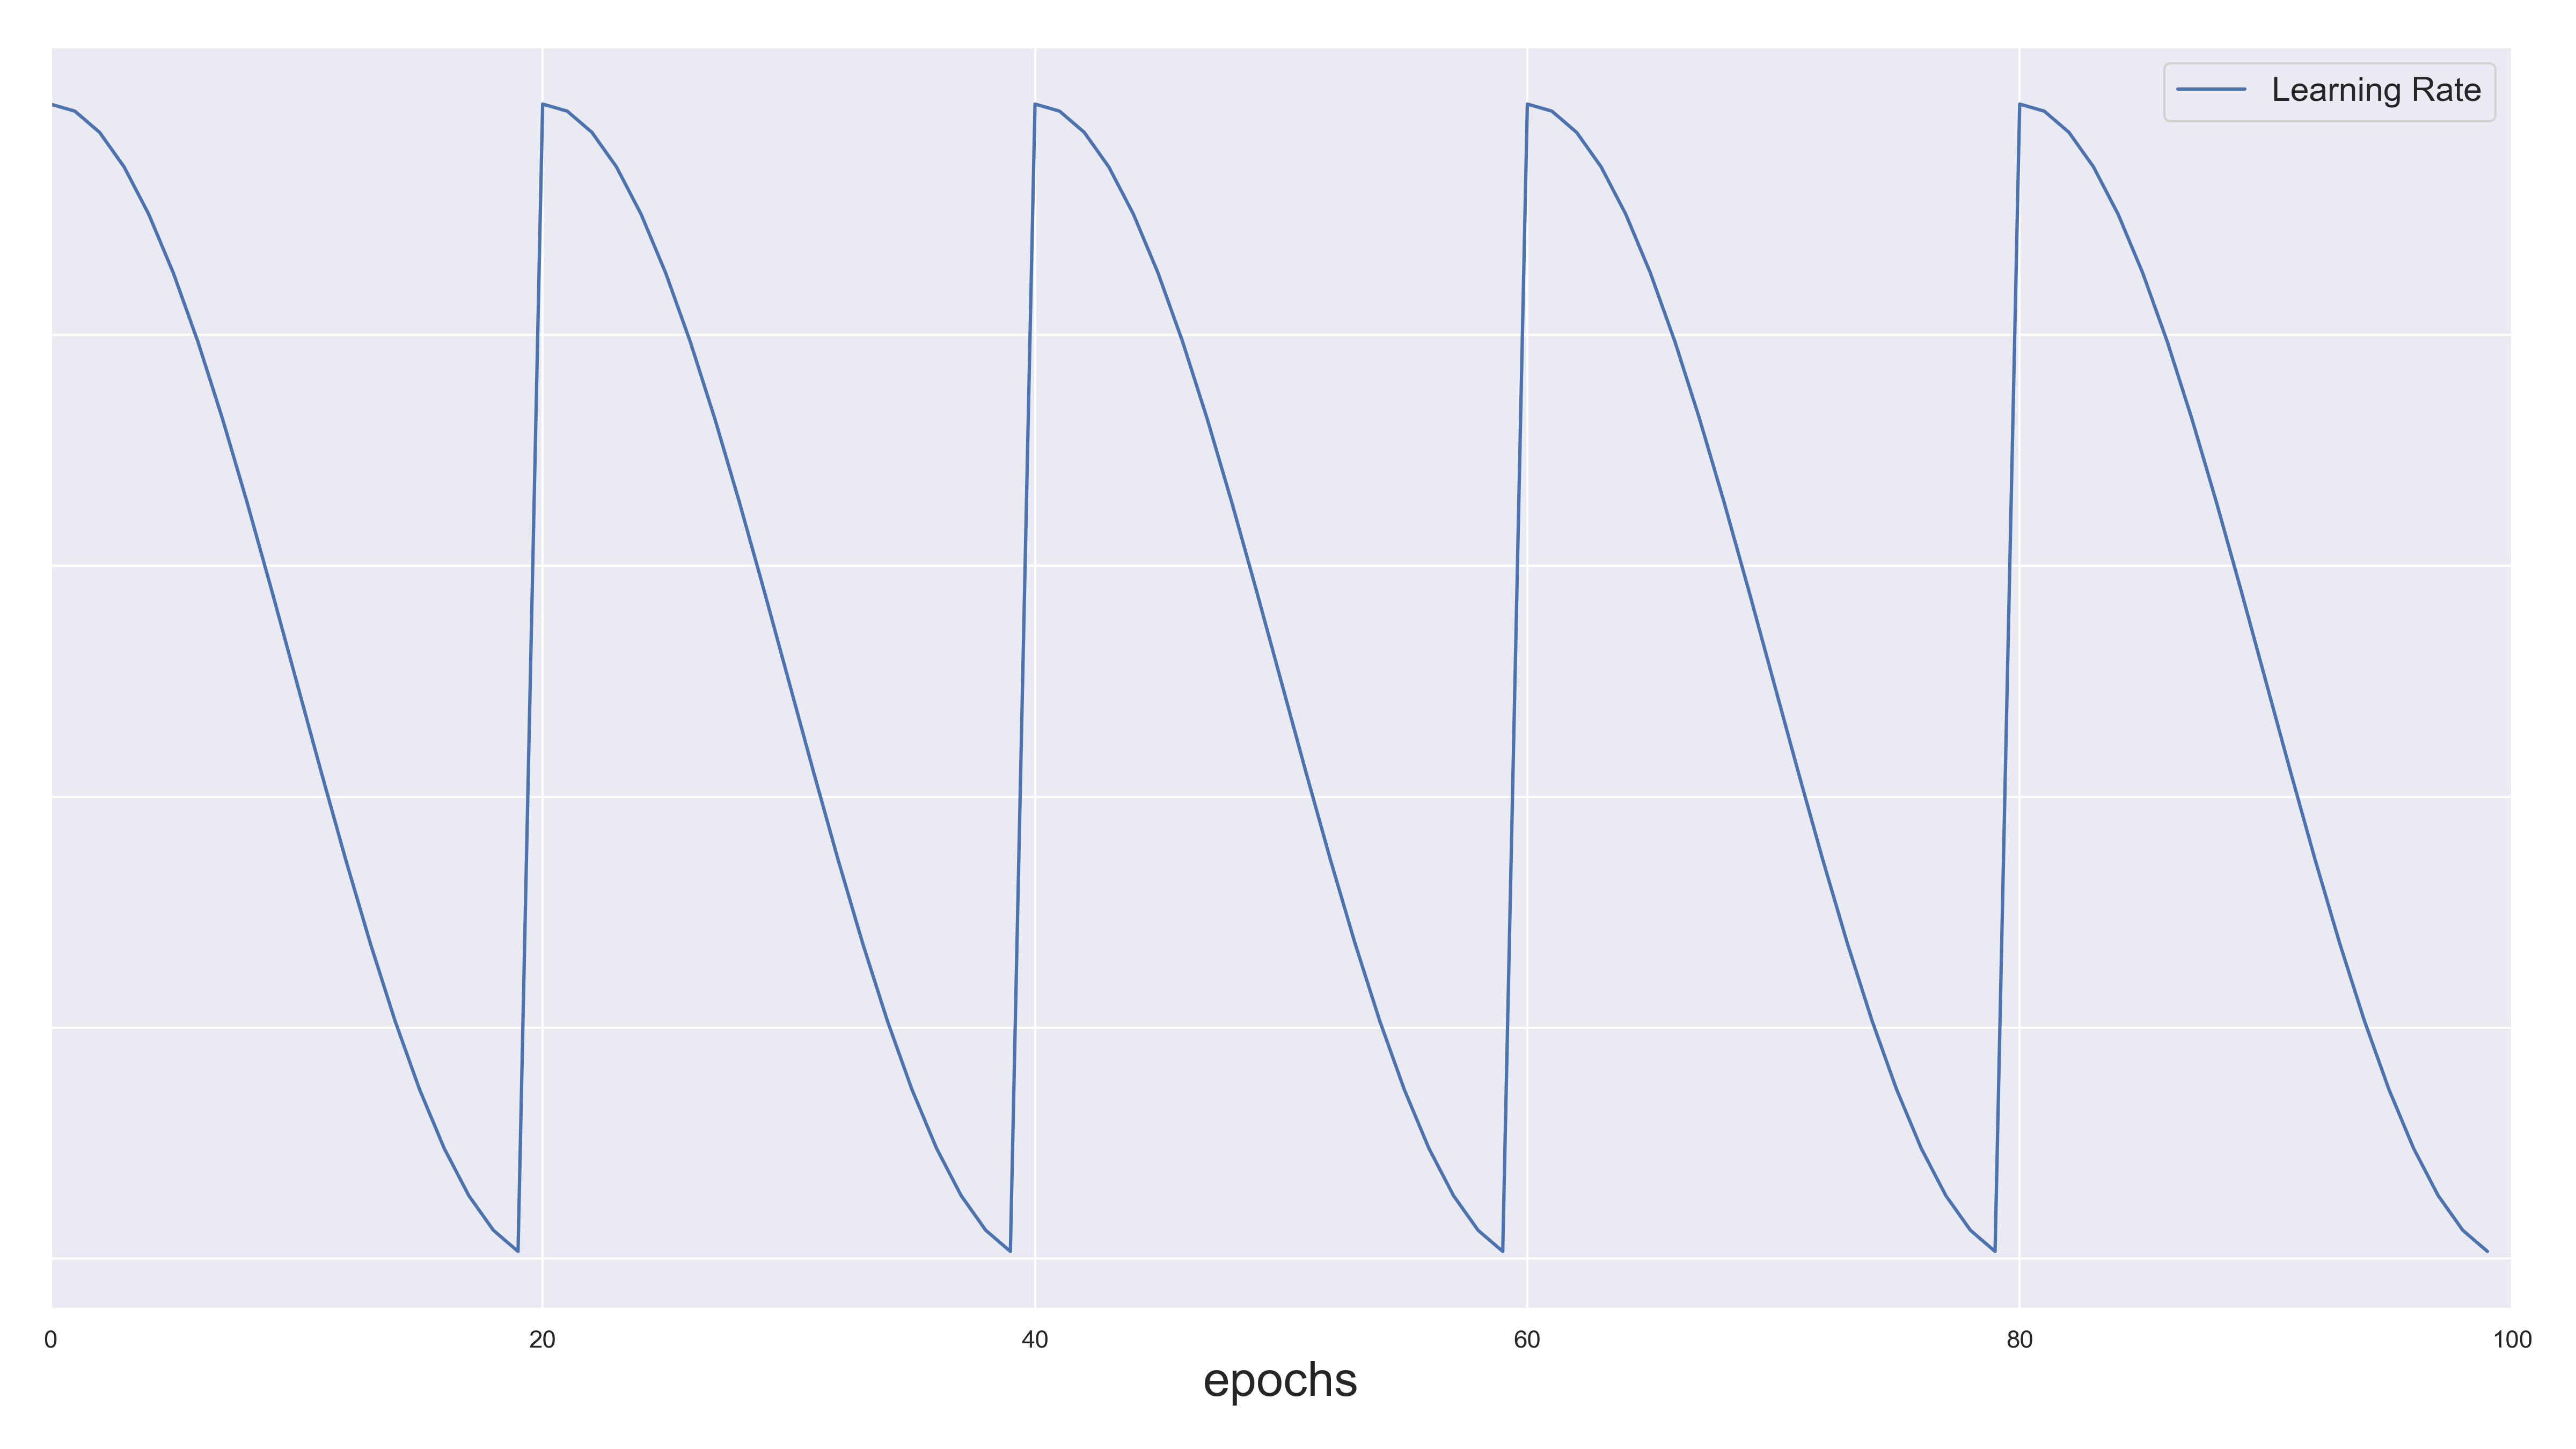
\includegraphics[width=.7\linewidth]{figures/lr.png}
			\captionof{figure}[Cosine Annealing Learning Rate]{Cosine Annealing Learning Rate} 
			\label{fig:cosineannealing}
		\end{minipage}
		
		\item[Batch Size] Batch Size are recommend to be between 1 and a few hundreds \cite{bengio_practical_2012}. To better utilize \gls{gpu}s, a batch size in the power of 2 gives better runtime, e.g. 32 to 256 \cite{goodfellow_deep_2016}. Larger batch sizes have been driven by advancements in parallelism \cite{dean_large_2012}, which can improve the training time. However, smaller batch sizes have shown better generalization performance due to a regularizing effect \cite{masters_revisiting_nodate}, which especially large models, that tends to overfit can benefit from \cite{goodfellow_deep_2016}. 
		
		A batch size of 16 was found to be the maximum power of 2 possible within the computational budget of 8Gb RAM. The standard choice of 32 caused memory exhaustion. However, a batch size of 16 provide decent training times and may provide additional regularization over 32. Smaller batch sizes were not experimented with, due to project length.
		
		\item[Datasets] \gls{min100} is a subset of the \gls{ilsvrc2012} dataset \cite{russakovsky_imagenet_2015}. \gls{min100} was created for this project, to reduce training time from several weeks to only days on available hardware. The subset is inspired by MiniImageNet \cite{vinyals_matching_2016}, that uses a subset of 100 classes with 600 samples for each class. \gls{min100} contains 100 out of 1.000 randomly sampled classes, which gives 127.300 out of 1.2m training samples, and 5.000 out of 50.000 validation samples. A full list of classes are found in the table \ref{tbl:min100}. 
		
		Compared to other sufficiently dense classification datasets e.g \gls{tinyimagenet} \cite{li_cs231n:_2018}, \gls{cifar10} and \gls{cifar100} \cite{krizhevsky_cifar-10_nodate}, the image sizes of these datasets are respectively $(64\times 64$), $(32\times 32)$, $(32\times 32)$ pixels, all of which are considered too small for this project. Other datasets such as MS COCO and Pascal VOC are better suited for object detection/segmentation, as images are not cropped to only focus on a single object, thus too challenging for classification. In fact Pascal VOC was initially tested, the model however, clearly overfitted the training data due to data sparsity. 
		
		\item[Image Augmentation] A models ability generalize a specific classification problem has a close connection with the number of available training samples. Data augmentation have shown to be powerful tool in order to virtually create more training data \cite{perez_effectiveness_2017}. Enlarging a training dataset by data augmentation, to virtually create new versions of an image, that are different from, yet still similar to the original image, without actually to annotate new samples \cite{goodfellow_deep_2016}. 
		Image augmentation involves transformations using tools from image processing to randomly apply noise injection, or color space transformations e.g. contrast and saturation distortions. Other approaches involves geometric transformations, such as simple transformations of flipping the image. More complex mehtods e.g. affine transformations create different image perspectives \cite{shorten_survey_2019}. Figure \ref{fig:augmentation} shows 64 random augmentations of an image of an elephant, achieved using \gls{imgaug} \cite{jung_imgaug:_nodate}.  
		
		\begin{minipage}[t]{\linewidth}
			\centering
			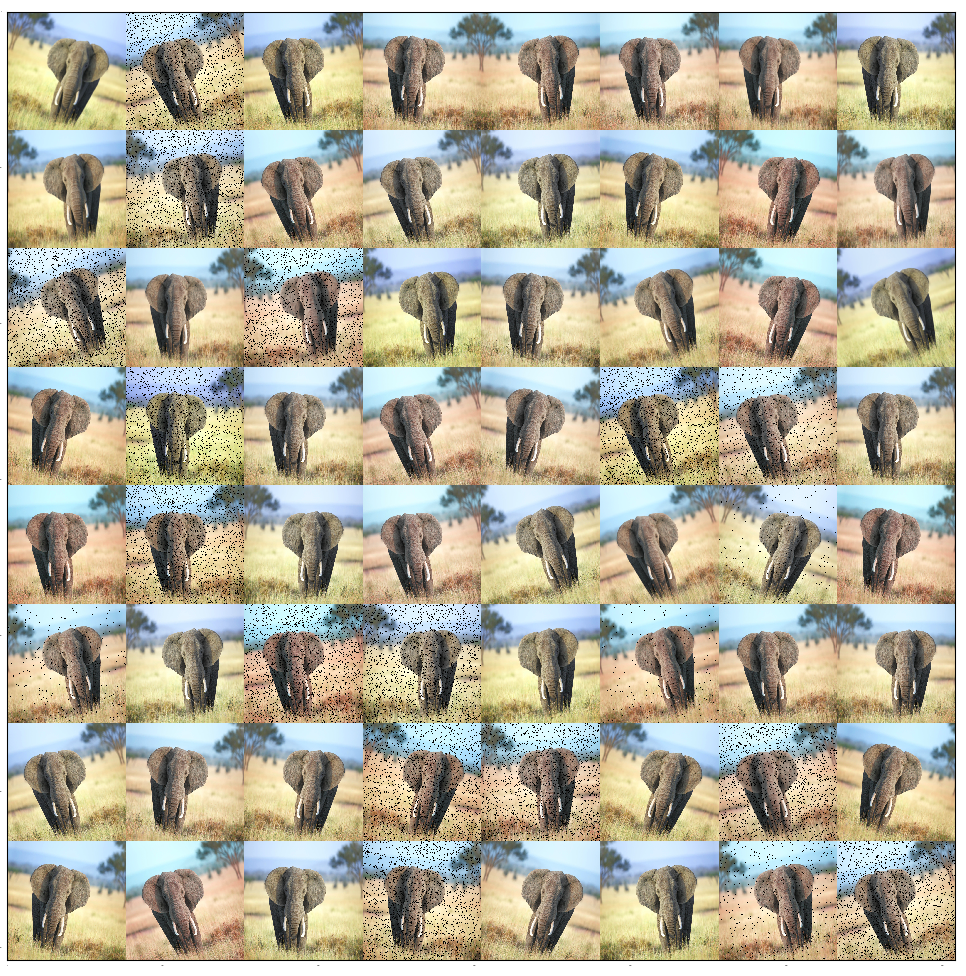
\includegraphics[width=.7\linewidth]{figures/augmentation/augmentation_high_resolution.png}
			\captionof{figure}[Image Augmentaion Example]{Image Augmentation of an elephant}
			\label{fig:augmentation}
		\end{minipage}
		
		New methods have been proposed where image transformations are learned to improve generalization e.g. AutoAugment \cite{cubuk_autoaugment:_2018}. Other methods involves actually enlarging the training dataset by synthetically creating more data using a \gls{gan}. \gls{gan}s can help overcome limited data given the available training data or a 3D model, by artificially constructing synthetic samples in different background, light setting and from alternate perspectives. However, these methods is a whole other area of research, and have been considered out of scope for this project.
		
		Methods that do not cover enriching the available training data, but alters the learning procedure are called regularization and covers; weight decay \cite{krogh_simple_nodate}, dropout \cite{srivastava_dropout:_nodate}, batch normalization \cite{ioffe_batch_2015} etc. We do not experiment with these regularization technique, but uses the settings already set in the implementation of the models.
		
		\item[Transfer Learning] Transfer learning is the procedure of using a pre-trained model to train on a new dataset, under the assumption, that features learned on one image dataset can be reused for another dataset \cite{yosinski_how_2014}. Typically models have been pre-trained on the ImageNet dataset. The density of the dataset enables models to learn general features suitable for other domains \cite{kornblith_better_2019}. Transfer learning are especially suitable, when the new data domain is of limited quantity and the similarities between the two data domains are strong. If the similarities are weak a model can be fine-tuned i.e., the shallow layers containing general features are frozen and only the deeper layers with more specialized features are optimized for the new data domain \cite{li_cs231n:_2018}. Thus, transfer learning can reduce the training time to learn general features of shallow layers, and possibly learn more specific features at deeper layers, adapted to the new dataset.
	\end{enumdescript}
	
	\item[Inference] The inference experiment have been conducted by letting all samples inference the model, the output and measured time of all exits have been logged and used for analysis in section \ref{sec:ee-results}. All hardware of table \ref{tbl:platforms} and all trained models of table \ref{tbl:models} have been used. The inference experiment does not require nearly the same amount of settings as the training does. Those required are listed here:
	\begin{enumdescript}
		\item[Batch Size] A batch size of 1 have been chosen to simulate a realistic scenario, and to measure time of each samples
		\item[Dataset] The validation dataset of \gls{min100} containing 5000 samples have been used.
	\end{enumdescript} 
	
\end{enumdescript}

\section{Results} \label{sec:ee-results}

The results section consists of two main parts. Section \ref{sec:ee-results-training} covers the result from training the \gls{dnn}s. Section \ref{sec:ee-results-inference} covers experimentation using our trained networks. 

\subsection{Training Results} \label{sec:ee-results-training}

We trained the three early exiting models \gls{bresnet}, \gls{bdensenet} and \gls{msdnet}, along with conventional versions of the \gls{resnet}101 and \gls{densenet}-121. The \gls{dnn}s were trained on the \gls{min100} training set.

We trained \gls{bresnet} using transfer learning from the ImageNet dataset. We froze the features of the network, hence we only trained the classifiers of the exits. Figure \ref{fig:frozen-b-resnet-miniimagenet-100} show the results from the training. The figure shows, that the features learned from a conventional single exit model, are not suitable for an early exit model. None of the intermediate classifiers are able to obtain acceptable accuracy on neither the training nor the validation set. The features for the shallower part of the network are not optimized for the early classifiers. This study clearly reveals the need to train the entire model, to obtain an early exit model with decent accuracy. As done in \cite{teerapittayanon_branchynet:_2016}, i.e. unfreezing the model, to allow the features of the model to be optimized for the intermediate classifiers of the early exits, show great improvements. Figure \ref{fig:b-resnet-miniimagenet-100} show the training results.

\begin{center}

\begin{minipage}[t]{.9\linewidth}

\begin{figure}
	\centering
	\captionsetup[subfigure]{justification=centering, farskip=1pt,captionskip=1pt}
	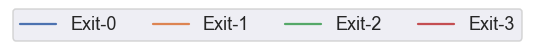
\includegraphics[width=.5\textwidth]{figures/training_plots/frozen_b-resnet_exit_legend}
	\subfloat[Train loss\label{fig:frozen-b-resnet-train-loss}]{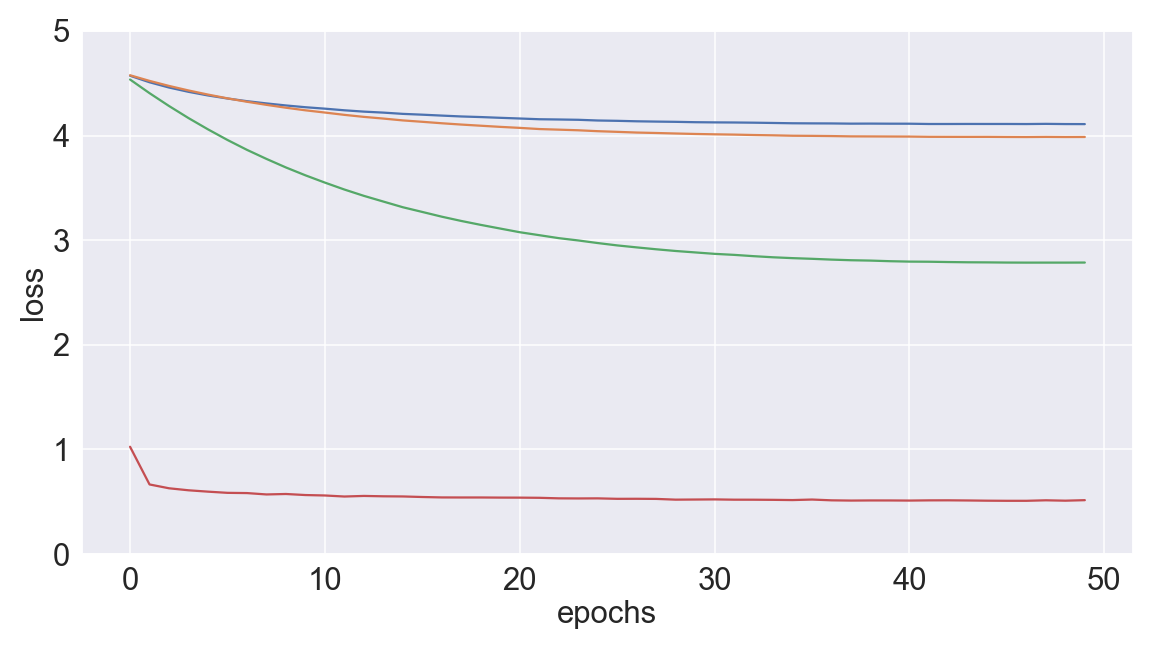
\includegraphics[width=.49\textwidth]{figures/training_plots/frozen_b-resnet_train-loss}}
	\subfloat[Test loss \label{fig:frozen-b-resnet-test-loss}]{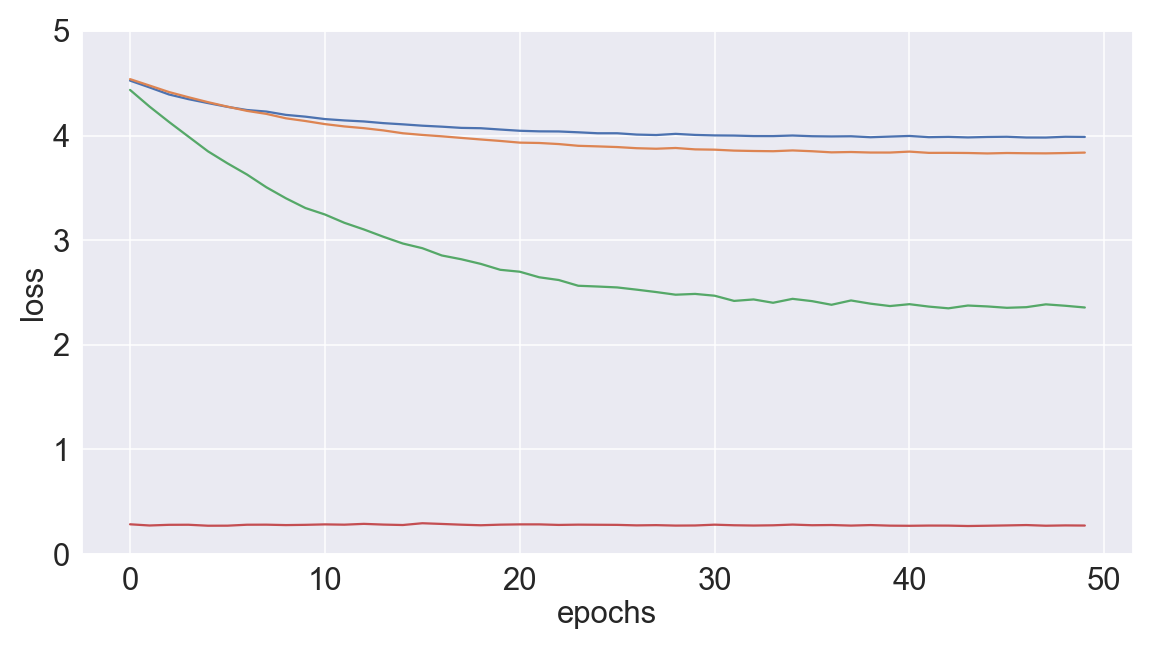
\includegraphics[width=.49\textwidth]{figures/training_plots/frozen_b-resnet_test-loss}}
	\hfill
	\subfloat[Train accuracy\label{fig:frozen-b-resnet-train-acc}]{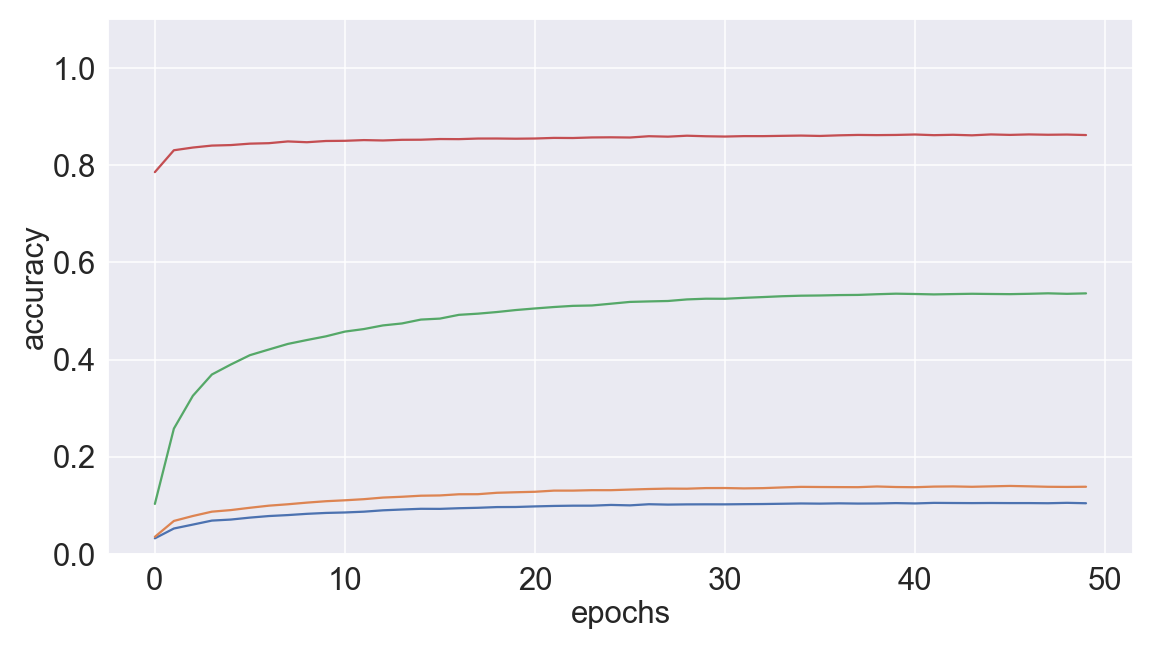
\includegraphics[width=.49\textwidth]{figures/training_plots/frozen_b-resnet_train-accuracy}}
	\subfloat[Test accuracy\label{fig:frozen-b-resnet-test-acc}]{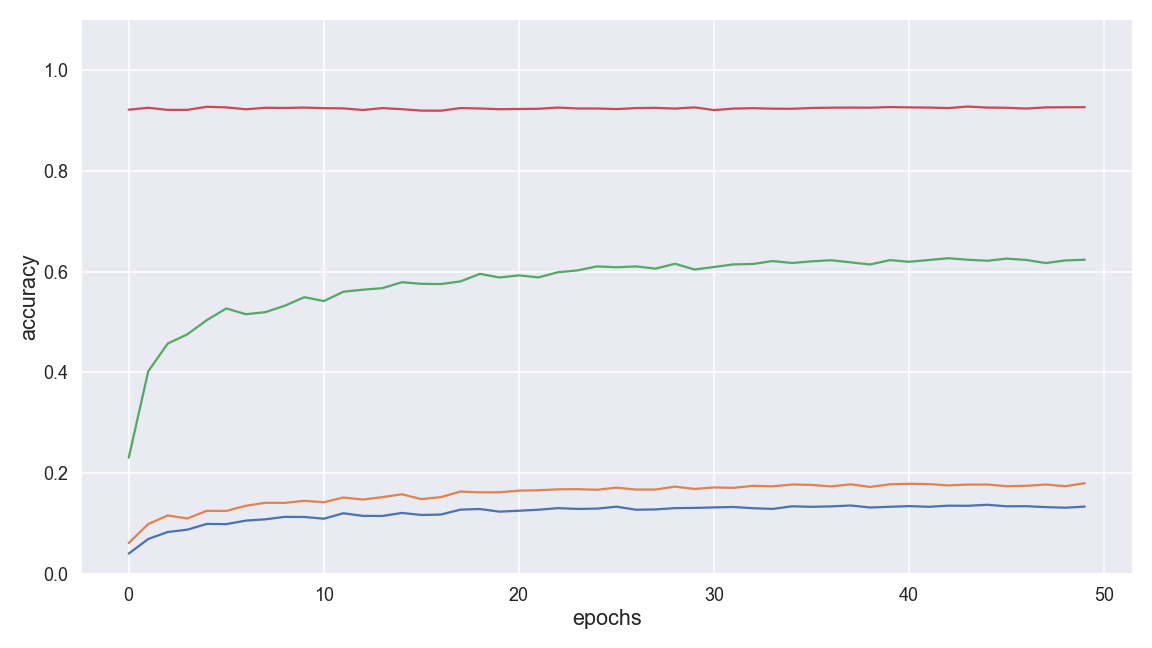
\includegraphics[width=.49\textwidth]{figures/training_plots/frozen_b-resnet_test-accuracy}}
	\caption[Frozen Bresnet Training summary]{Frozen \gls{bresnet} Training summary: shows the progression of model attributes over times of epochs, \protect\subref{fig:frozen-b-resnet-train-loss} train loss, \protect\subref{fig:frozen-b-resnet-test-loss} test loss, \protect\subref{fig:frozen-b-resnet-train-acc} train accuracy, \protect\subref{fig:frozen-b-resnet-test-acc}, test accuracy.}
	\label{fig:frozen-b-resnet-miniimagenet-100}
\end{figure}
\begin{figure}
	\centering
	\captionsetup[subfigure]{justification=centering, farskip=1pt,captionskip=1pt}
	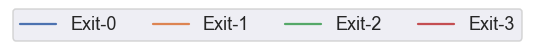
\includegraphics[width=.5\textwidth]{figures/training_plots/b-resnet_exit_legend}
	\subfloat[Train loss\label{fig:b-resnet-train-loss}]{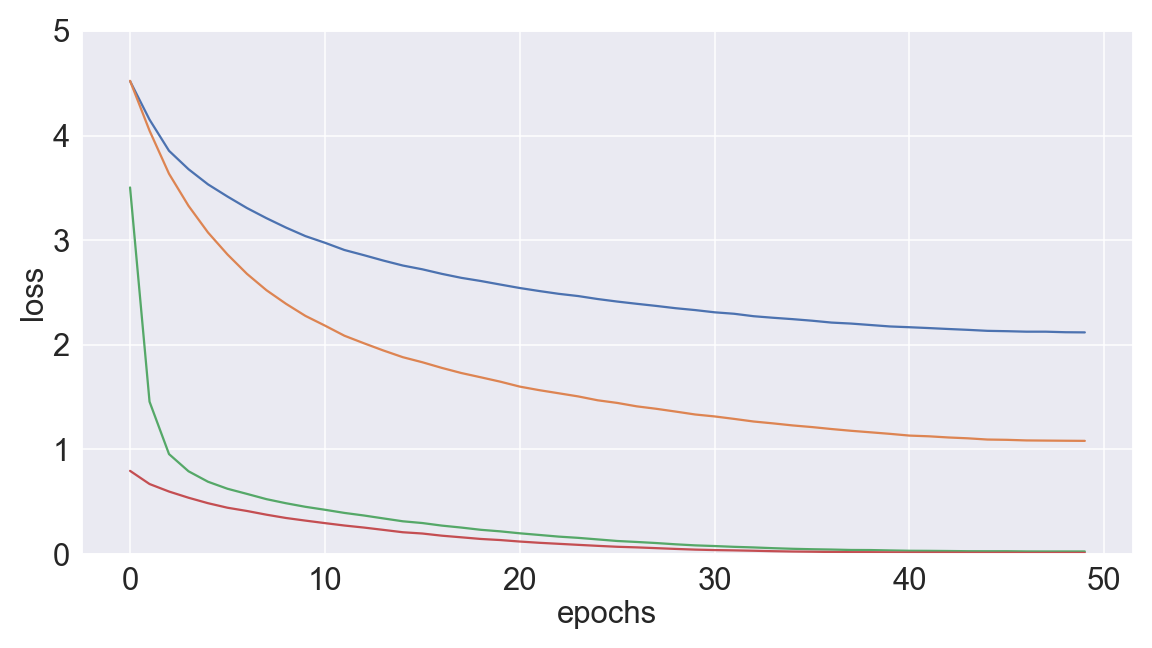
\includegraphics[width=.49\textwidth]{figures/training_plots/b-resnet_train-loss}}
	\subfloat[Test loss \label{fig:b-resnet-test-loss}]{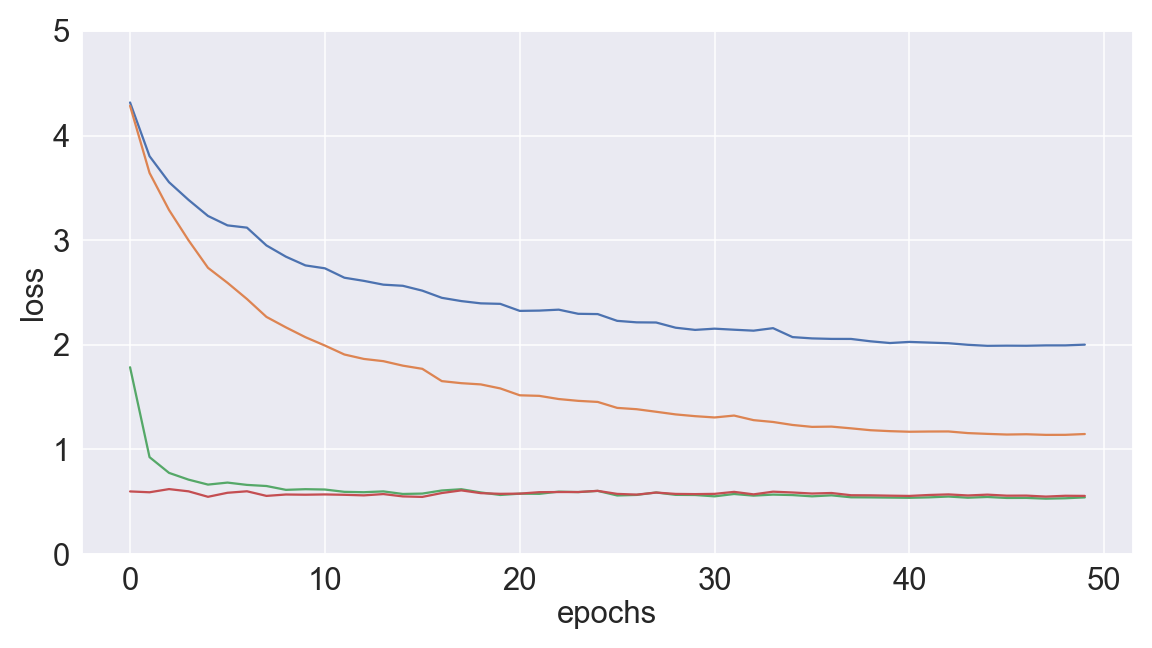
\includegraphics[width=.49\textwidth]{figures/training_plots/b-resnet_test-loss}}
	\hfill
	\subfloat[Train accuracy\label{fig:b-resnet-train-acc}]{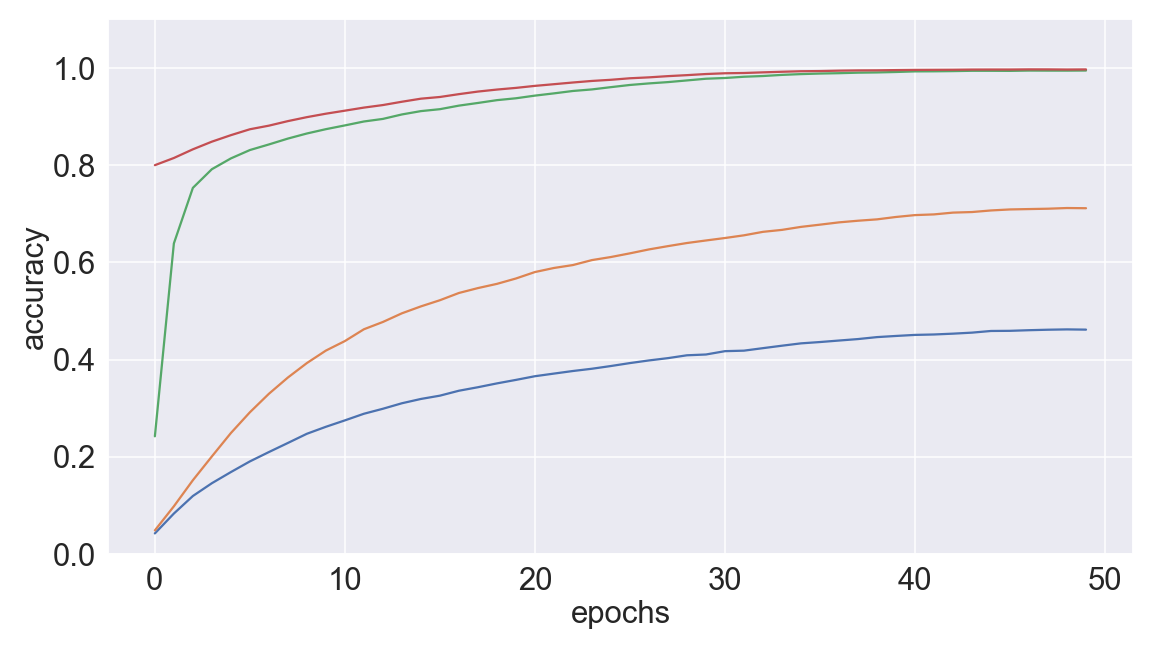
\includegraphics[width=.49\textwidth]{figures/training_plots/b-resnet_train-accuracy}}
	\subfloat[Test accuracy\label{fig:b-resnet-test-acc}]{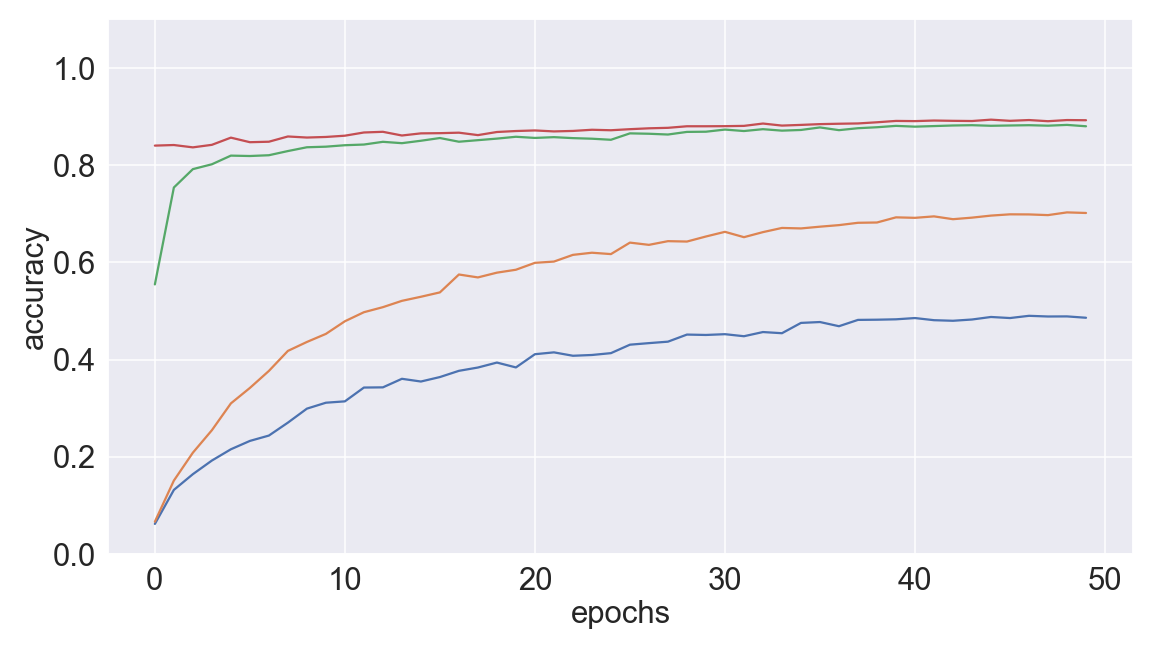
\includegraphics[width=.49\textwidth]{figures/training_plots/b-resnet_test-accuracy}}
	\caption[B-ResNet Training summary]{B-ResNet Training summary: shows the progression of model attributes over times of epochs, \protect\subref{fig:b-resnet-train-loss} train loss, \protect\subref{fig:b-resnet-test-loss} test loss, \protect\subref{fig:b-resnet-train-acc} train accuracy, \protect\subref{fig:b-resnet-test-acc}, test accuracy.}
	\label{fig:b-resnet-miniimagenet-100}
\end{figure}
\end{minipage}
\end{center}

Table \ref{tbl:frozen-vs-unfrozen} summarizes the validation accuracy gain for each exit when training the entire model. Comparing the two show, that we are able to improve the accuracy at early exits, thus the features located in the shallower part of the model now provides information that enables the classifiers to better discriminate the classes. 

\begin{longtabu}{>{\bfseries}X[2]|X[r]|X[r]|X[r]|X[r]}
	\caption[Comparison of Transfer Learning Approaches]{Comparison of transfer learning approaches frozen model vs. fine-tuning on validation accuracy} \label{tbl:frozen-vs-unfrozen} \\
	\toprule
	\rowfont{\bfseries}
	Model & Exit-0 & Exit-1 & Exit-2 & Exit-3 \tabularnewline
	\bottomrule
	\endfirsthead
	\multicolumn{3}{@{}l}{\textbf{\textcolor{black}{Table \ref{tbl:frozen-vs-unfrozen}:}} continued}\\
	\toprule
	\rowfont{\bfseries}
	Model & Exit-0 & Exit-1 & Exit-2 & Exit-1 \tabularnewline
	\bottomrule
	\endhead % all the lines above this will be repeated on every page
	\bottomrule
	\multicolumn{3}{@{}l}{continued \ldots}\\
	\endfoot
	\hline
	\endlastfoot
	Frozen B-\gls{resnet}	& 0.14	& 0.18	& 0.63 & 0.93 \tabularnewline
	\hline
	Unfrozen B-\gls{resnet}	& 0.49 	& 0.70 & 0.88 & 0.89 \tabularnewline
	\hline
	Gain & 3.50 & 3.89 & 1.40 &  0.96  \tabularnewline							
	\bottomrule
\end{longtabu}

The accuracy at early exits classifiers are greatly improved by 1.4 times to almost 3.9 times. However, the accuracy of the final classifier are reduced by 0.96 times. The reduction in accuracy may be caused by;
\begin{enumerate}
	\item The features of the third and largest resolution block just before exit-2, see table \ref{tbl:resnet101}, may be optimized too much for exit-2, thus collapses the information, that the last block should use to learn more descriptive features. 
	\item It could be a sign of overfitting, due to the size of dataset is only $\frac{1}{10}$ of the dataset used to train the original model. 
\end{enumerate}

However, the last two exits obtain a training accuracy close to 1. However, there is no notable degradation in validation loss or accuracy, which would have been the clearest sign of overfitting. We did also train conventional versions of the two models on the same datasets, and since both models are able to obtain over 0.9 in accuracy, we argue, that the most probable reason is optimization to earlier exit, as the same trend is shown in \cite{huang_multi-scale_2017}.

Figure \ref{fig:b-densenet-miniimagenet-100} show the training result of B-\gls{densenet}. B-\gls{densenet} always has a gain in accuracy by continuing the inference process to the next exit, and are also able to achieve better accuracy at earlier exits than B-\gls{resnet}. However, again at the cost of less accurate end exit. Figure \ref{fig:msdnet-miniimagenet-100} show the results of training the \gls{msdnet}. The model specifically designed for early exiting shows indeed improvements for classifiers at early exit, but the overall accuracy i.e. the accuracy of the final classifier is slightly smaller compared to the other two models.

\begin{center}
	\begin{minipage}[t]{.9\linewidth}

\begin{figure}
	\centering
	\captionsetup[subfigure]{justification=centering, farskip=1pt,captionskip=1pt}
	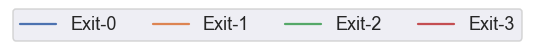
\includegraphics[width=.5\textwidth]{figures/training_plots/b-densenet_exit_legend}
	\subfloat[Train loss\label{fig:b-densenet-train-loss}]{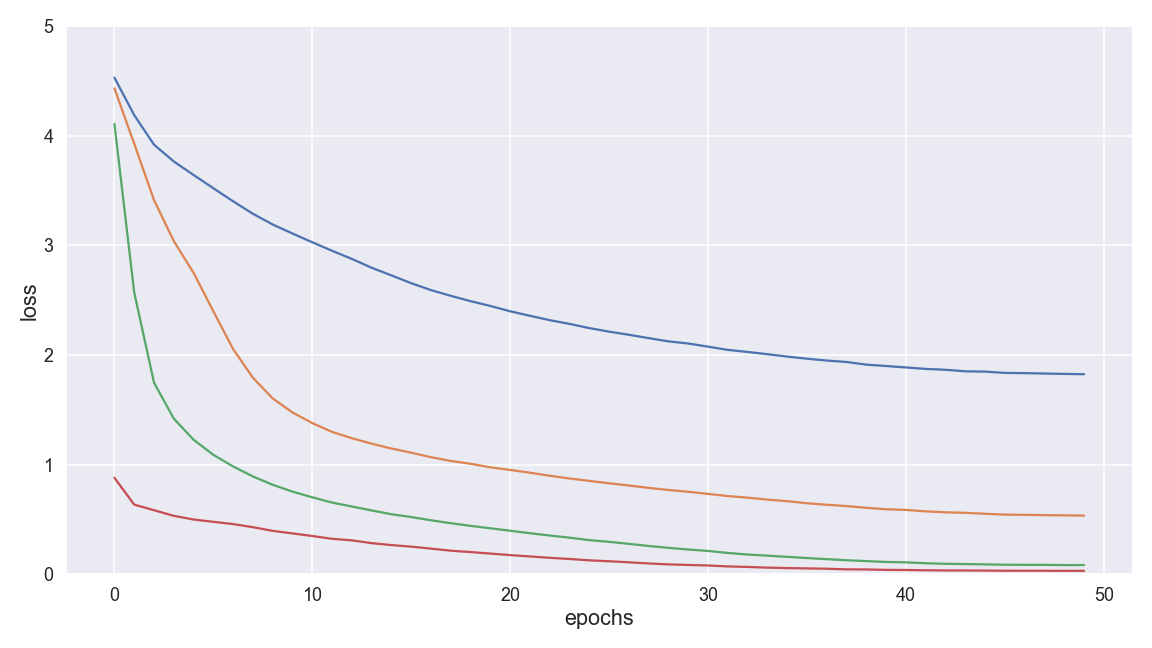
\includegraphics[width=.49\textwidth]{figures/training_plots/b-densenet_train-loss}}
	\subfloat[Test loss \label{fig:b-densenet-test-loss}]{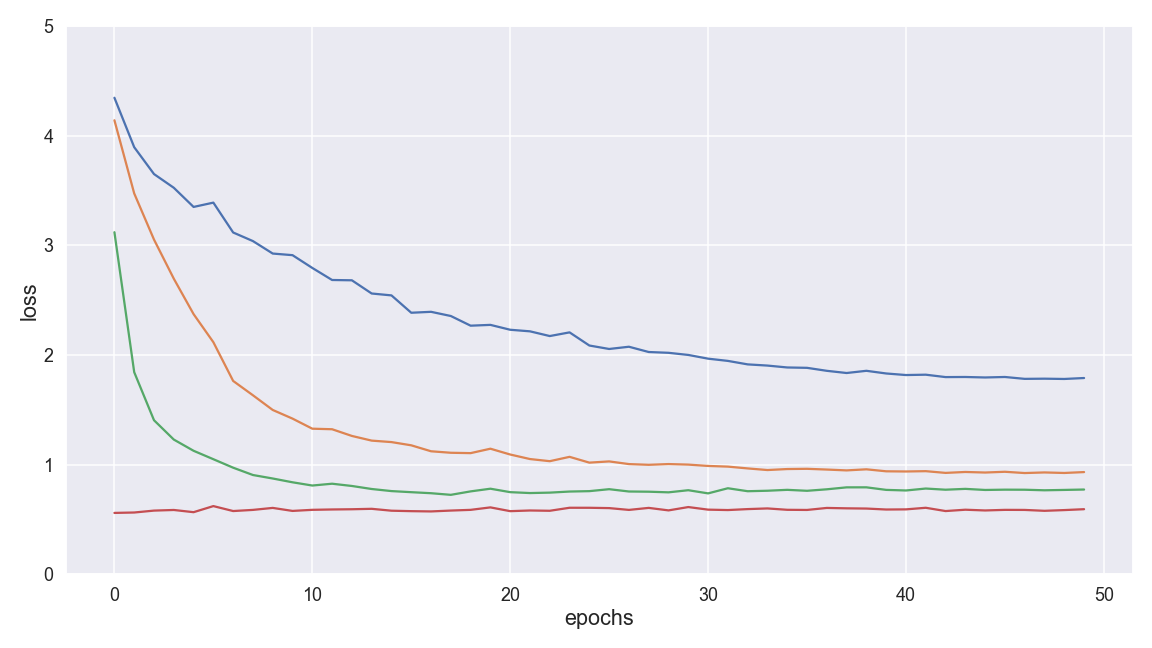
\includegraphics[width=.49\textwidth]{figures/training_plots/b-densenet_test-loss}}
	\hfill
	\subfloat[Train accuracy\label{fig:b-densenet-train-acc}]{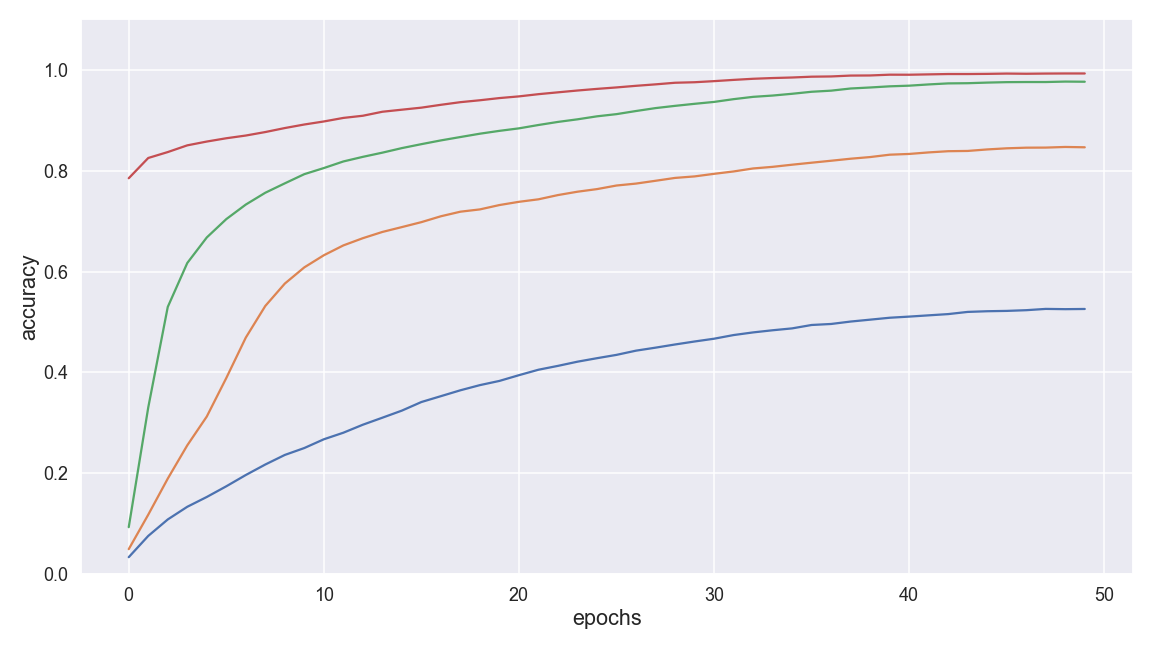
\includegraphics[width=.49\textwidth]{figures/training_plots/b-densenet_train-accuracy}}
	\subfloat[Test accuracy\label{fig:b-densenet-test-acc}]{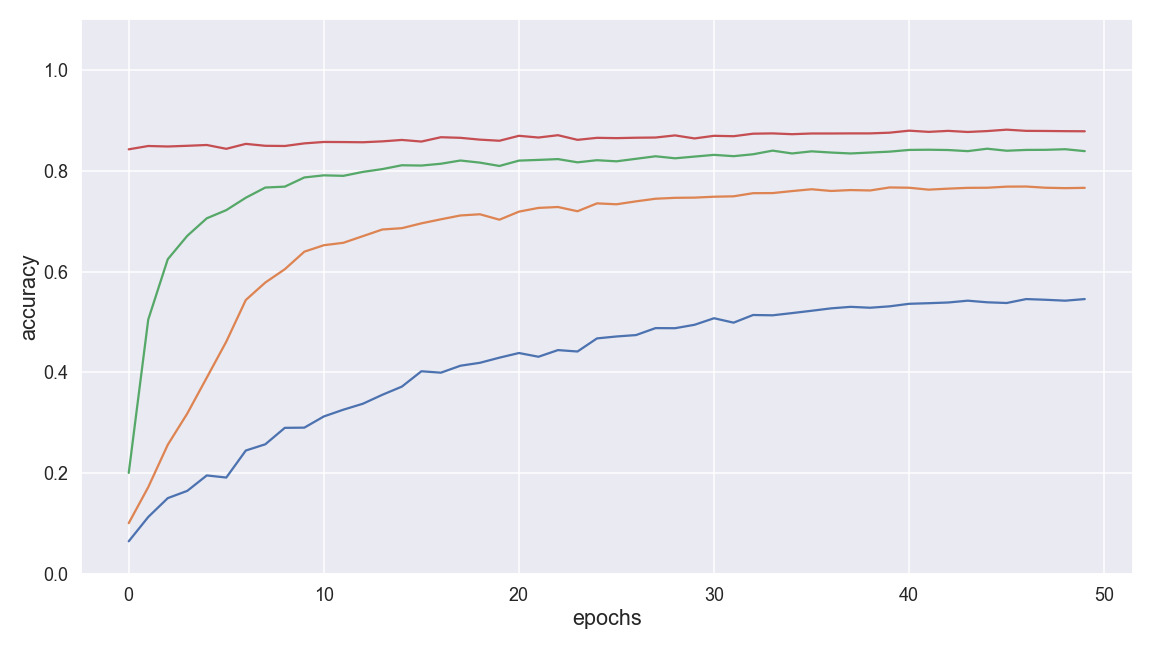
\includegraphics[width=.49\textwidth]{figures/training_plots/b-densenet_test-accuracy}}
	\caption[B-densenet Training summary]{B-densenet Training summary: shows the progression of model attributes over times of epochs, \protect\subref{fig:b-densenet-train-loss} train loss, \protect\subref{fig:b-densenet-test-loss} test loss, \protect\subref{fig:b-densenet-train-acc} train accuracy, \protect\subref{fig:b-densenet-test-acc}, test accuracy.}
	\label{fig:b-densenet-miniimagenet-100}
\end{figure}

\begin{figure}
	\centering
	\captionsetup[subfigure]{justification=centering, farskip=1pt,captionskip=1pt}
	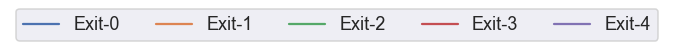
\includegraphics[width=.5\textwidth]{figures/training_plots/msdnet_exit_legend}
	\subfloat[Train loss\label{fig:msdnet-train-loss}]{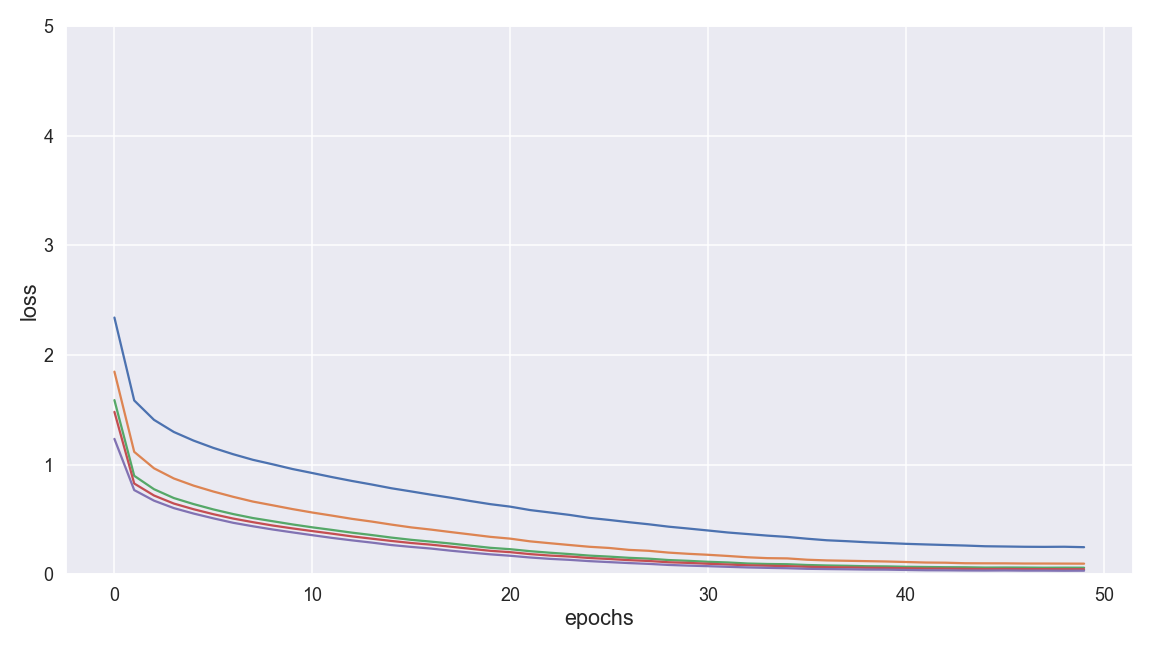
\includegraphics[width=.49\textwidth]{figures/training_plots/msdnet_train-loss}}
	\subfloat[Test loss \label{fig:msdnet-test-loss}]{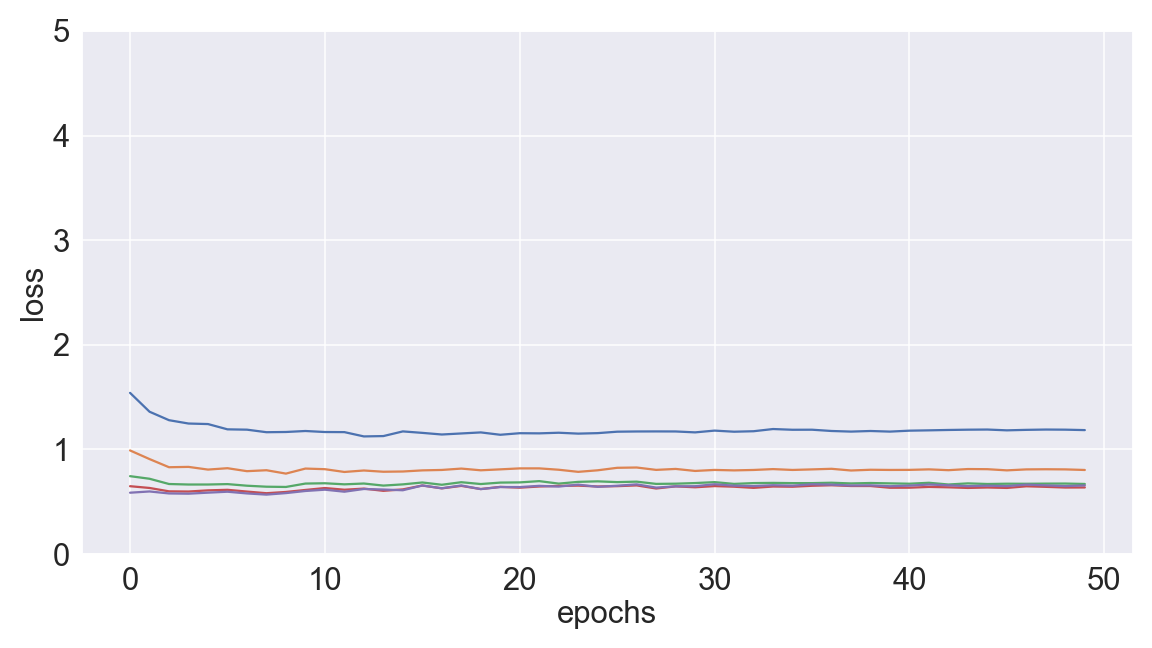
\includegraphics[width=.49\textwidth]{figures/training_plots/msdnet_test-loss}}
	\hfill
	\subfloat[Train accuracy\label{fig:msdnet-train-acc}]{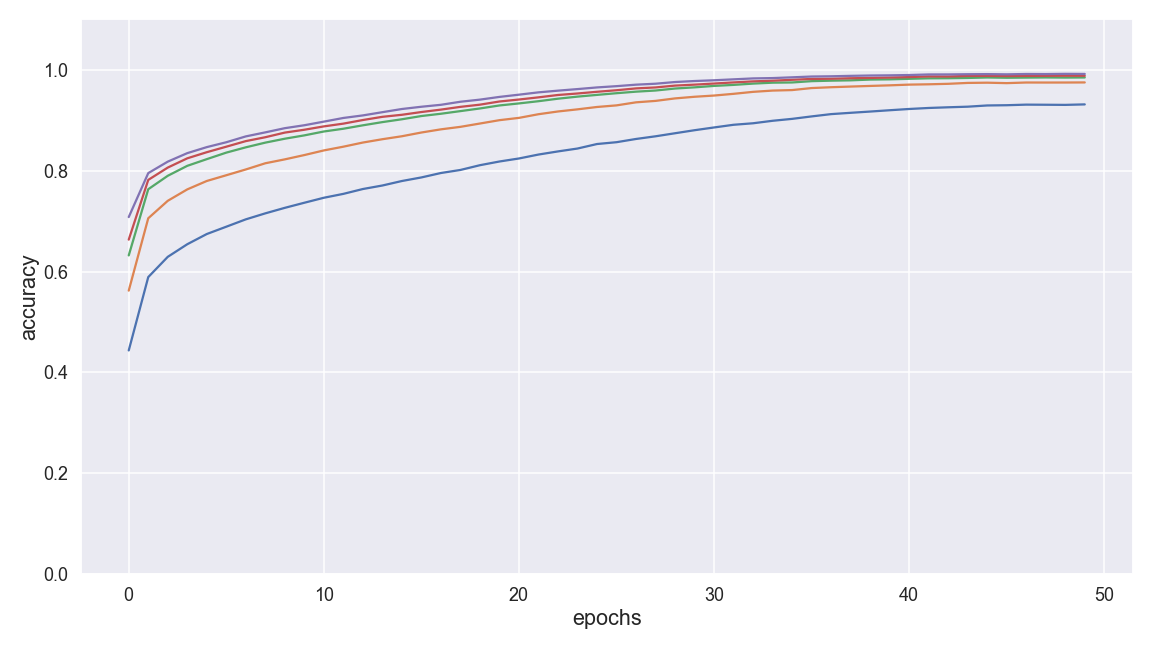
\includegraphics[width=.49\textwidth]{figures/training_plots/msdnet_train-accuracy}}
	\subfloat[Test accuracy\label{fig:msdnet-test-acc}]{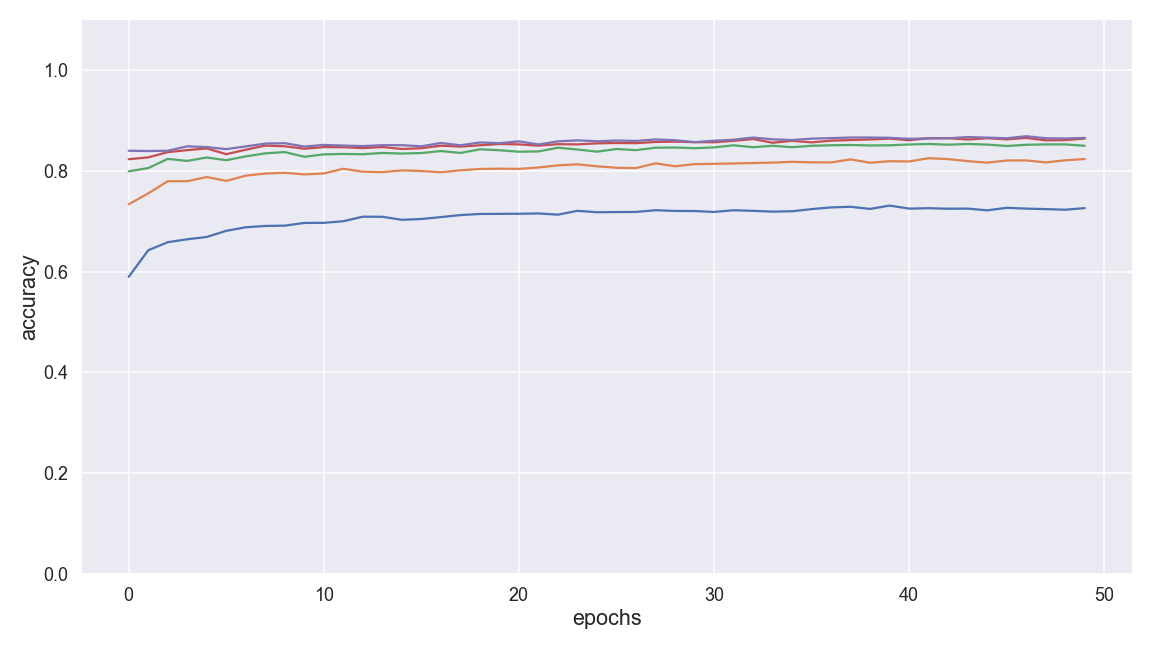
\includegraphics[width=.49\textwidth]{figures/training_plots/msdnet_test-accuracy}}
	\caption[MSDNet Training summary]{MSDNet Training summary: shows the progression of model attributes over times of epochs, \protect\subref{fig:msdnet-train-loss} train loss, \protect\subref{fig:msdnet-test-loss} test loss, \protect\subref{fig:msdnet-train-acc} train accuracy, \protect\subref{fig:msdnet-test-acc}, test accuracy.}
	\label{fig:msdnet-miniimagenet-100}
\end{figure}
	\end{minipage}
\end{center}

\subsection{Inference Results} \label{sec:ee-results-inference}

In this section we evaluate the accuracy of the early exit models. All validation samples are inferred to all model of table \ref{tbl:models}. Figure \ref{fig:exit-accuracy} show the top-1 and top-5 accuracy of all exits of the three models.  

\begin{figure}
	\centering
	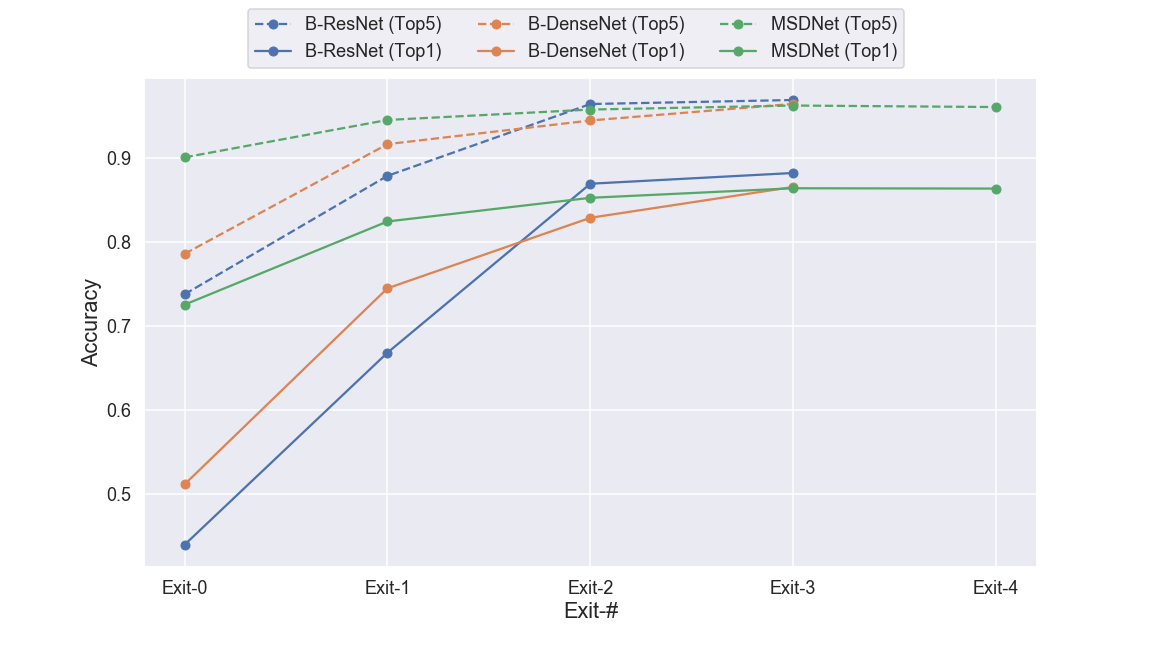
\includegraphics[width=.8\linewidth]{figures/inference_plots/accuracy-comparison}
	\caption[Accuracy of Early Exit Models]{Accuracy of Early Exit Models, B-\gls{resnet}, B-\gls{densenet} and \gls{msdnet}}
	\label{fig:exit-accuracy}
\end{figure}

The models achieve higher accuracy, as the samples are predicted by a deeper exit in the network, as the increasingly complex features deep within the networks have more discriminative characteristics. Table \ref{tbl:validation-comparison} compares the top-1 accuracy  of the three models. As the two last exits of \gls{bresnet} is almost equally accurate, not much gain is obtained by running the model all the way to the end.  

\begin{longtabu}{>{\bfseries}X[2]|X|X|X|X|X}
	\caption[Early Exiting Top-1 Accuracy]{Early Exiting Validation Accuracy from Training} \label{tbl:validation-comparison} \\
	\toprule
	\rowfont{\bfseries}
	Model & Exit-0 & Exit-1 & Exit-2 & Exit-3 & Exit-4 \tabularnewline
	\bottomrule
	\endfirsthead
	\multicolumn{3}{@{}l}{\textbf{\textcolor{black}{Table \ref{tbl:frozen-vs-unfrozen}:}} continued}\\
	\toprule
	\rowfont{\bfseries}
	Model & Exit-0 & Exit-1 & Exit-2 & Exit-3 & Exit-4 \tabularnewline
	\bottomrule
	\endhead % all the lines above this will be repeated on every page
	\bottomrule
	\multicolumn{3}{@{}l}{continued \ldots}\\
	\endfoot
	\hline
	\endlastfoot
	B-\gls{resnet} & 0.49 	& 0.70 & 0.88 & 0.89 & N/A \tabularnewline
	\hline
	B-\gls{densenet}	& 0.55 	& 0.77 & 0.84 & 0.88 & N/A \tabularnewline
	\hline
	\gls{msdnet} & 0.73 & 0.82 & 0.85 &  0.87 & 0.87 \tabularnewline							
	\bottomrule
\end{longtabu}

The results justifies the assumption for early exiting, as close to 50 \% of the samples can be accurately classified at the first exit of any of the models.The importance of the densely connected layers for an early exit model, as found in \cite{huang_multi-scale_2017} becomes apparent in table \ref{tbl:validation-comparison}. The accuracy for early exits in both \gls{bdensenet} and \gls{msdnet} substantiates this claim. However, the end-exit of \gls{bresnet} achieves superior top-1 accuracy compared to the other models. In the next section we study the inference time of the models.  

\subsubsection{Inference Time Analysis}

We measure the inference time for each exits, of all 5 models, on the three platforms. Table \ref{tbl:inference-stats} show the mean, standard deviation, minimum and maximum for the model inference time on the platforms. The early exiting framework only adds a small delay overhead from the early exit classifiers, when comparing the last exit runtimes of the \gls{branchynet} models, with its conventional pendant. For the \gls{gpu}-enabled platforms, \gls{gpu} Workstation Jetson TX2, only additional 1.1ms and 2.4ms respectively on average. Whereas on the NUC the \gls{bresnet} is 7.5 ms slower, yet the \gls{densenet} is only slightly slower by 0.01 ms.   

\begin{footnotesize}
\begin{longtabu}{>{\bfseries}X[2.6]|[1pt]X[r]|X[0.8r]|X[r]|X[1.2r]|[1pt]X[r]|X[0.7r]|X[r]|X[1.2r]|[1pt]X[r]|X[0.7r]|X[r]|X[1.2r]}
	\caption[Inference time statistics]{Inference time statistics (mean, standard deviation, minimum, maximum) of the five models on the three platforms }\label{tbl:inference-stats} \\
	\toprule
	\rowfont{\bfseries}
	& \multicolumn4{c|[1pt]}{GPU Workstation} &  \multicolumn4{c|[1pt]}{Jetson TX2} & \multicolumn4{c}{Intel NUC} \tabularnewline
	\tabucline{2-13}
	\rowfont{\bfseries} Model & Mean & Std.  & Min & Max & Mean & Std. & Min & Max & Mean & Std.  & Min & Max  \tabularnewline
	\hline
	\endfirsthead
	\multicolumn{3}{@{}l}{\textbf{\textcolor{black}{Table \ref{tbl:inference-stats}:}} continued}\\
	\toprule
	\rowfont{\bfseries}
	& \multicolumn4{c|[1pt]}{GPU Workstation} &  \multicolumn4{c|[1pt]}{Jetson TX2} & \multicolumn4{c}{Intel NUC} \tabularnewline
	\tabucline{2-13}
	\rowfont{\bfseries} Model & Mean & Std.  & Min & Max & Mean & Std.  & Min & Max & Mean & Std.  & Min & Max  \tabularnewline
	\hline
	\endhead % all the lines above this will be repeated on every page
	\hline
	\multicolumn{3}{@{}l}{continued \ldots}\\
	\endfoot
	\hline
	\endlastfoot
	ResNet  	& 36.01 & 1.72 & 33.24 & 69.02 & 64.19 & 1.95 & 61.28 & 110.17 & 215.76 & 21.98 & 132.98 & 275.55 \tabularnewline
	\hline
	DenseNet 	& 47.74 & 1.95 & 4.48 & 86.88 & 70.48 & 3.04 & 59.56 & 132.45 &  72.30 &  2.61 &  69.02 & 107.63 \tabularnewline
	\hline
	B-ResNet & & & &&&&&&&& &  \tabularnewline 
	\hspace{3mm} Exit-0 &  4.20 & 0.63 &  3.81 &  39.40 &  8.61 & 0.31 &  8.39 &  15.54 &  38.25 &  1.85 &  29.26 &  74.94 \tabularnewline
	\hspace{3mm} Exit-1 &  9.40 & 1.28 &  8.19 &  70.23 & 19.30 & 1.08 & 16.42 &  38.41 &  66.69 &  3.15 &  50.41 & 110.80 \tabularnewline
	\hspace{3mm} Exit-2 & 33.59 & 2.78 & 30.25 & 103.55 & 56.77 & 2.73 & 52.34 & 102.58 & 196.43 &  8.81 & 150.11 & 254.86 \tabularnewline
	\hspace{3mm} Exit-3 & 37.14 & 2.94 & 33.65 & 109.94 & 67.04 & 2.86 & 62.47 & 116.74 & 223.32 & 10.35 & 170.95 & 289.67 \tabularnewline
	\hline
	B-DenseNet &  & & &&&&&&&& & \tabularnewline
	\hspace{3mm} Exit-0 &  5.83 & 1.09 &  5.15 &  54.61 & 11.05 & 0.48 & 10.52 & 17.31 &  28.83 & 1.59 & 26.05 & 41.93 \tabularnewline
	\hspace{3mm} Exit-1 & 17.03 & 1.89 & 14.60 &  76.78 & 30.26 & 2.02 & 23.75 & 47.54 &  46.71 & 2.31 & 43.47 & 71.85 \tabularnewline
	\hspace{3mm} Exit-2 & 36.31 & 3.01 & 32.72 & 104.79 & 55.38 & 3.22 & 48.10 & 87.81 &  64.26 & 2.80 & 60.65 & 99.41 \tabularnewline
	\hspace{3mm} Exit-3 & 49.14 & 3.36 & 45.13 & 127.07 & 72.41 & 3.89 & 64.77 & 120.29 & 72.31 & 2.97 & 68.37 & 112.06 \tabularnewline
	\hline
	MSDNet & & &&&&&&&&&& \tabularnewline
	\hspace{3mm} Exit-0 & 24.14 & 1.59 & 21.53 &  67.38 &  40.37 & 2.77 & 29.36 & 209.89 & 19.99 & 1.27 & 16.99 &  35.12 \tabularnewline
	\hspace{3mm} Exit-1 & 42.24 & 2.54 & 38.87 & 119.85 &  65.18 & 4.29 & 53.34 & 267.19 & 32.82 & 2.38 & 29.03 & 103.19 \tabularnewline
	\hspace{3mm} Exit-2 & 55.59 & 2.82 & 51.90 & 143.30 &  83.81 & 5.43 & 71.39 & 312.55 & 42.89 & 3.03 & 38.72 & 130.52 \tabularnewline
	\hspace{3mm} Exit-3 & 64.49 & 2.99 & 60.59 & 156.26 &  96.53 & 6.26 & 83.68 & 345.67 & 50.10 & 3.43 & 45.66 & 145.75 \tabularnewline
	\hspace{3mm} Exit-4 & 68.87 & 3.11 & 64.85 & 165.90 & 103.29 & 6.65 & 90.14 & 361.02 & 56.02 & 3.62 & 51.28 & 154.08 \tabularnewline
	\bottomrule
\end{longtabu}

\end{footnotesize}

The inference time are very different on the three platforms, and is very much dependent on the hardware characteristics. Figure \ref{fig:inference-time-dist} plots the inference timing for each exit of the models, on the 3 platforms as histograms. Clearly the \gls{gpu-ws} is in general the fastest, due to more computing resources. Especially the \gls{resnet}-based models achieve far superior times on this platform. The \gls{nuc} is generally the slowest. Note, the runtime of the \gls{msdnet} on the \gls{nuc} is far superior compared to the two \gls{gpu}-enabled platforms, this result is elaborated upon in section \ref{sec:ee-summary}.

\begin{figure}
	\begin{minipage}{\textwidth}
		\centering
		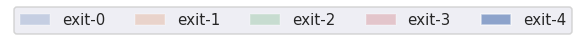
\includegraphics[width=.5\linewidth]{figures/inference_plots/time_dist_legend}
	\end{minipage}
	\begin{minipage}{0.33\textwidth}
		\captionsetup[subfigure]{farskip=0pt,captionskip=0pt, justification=centering}
		\centering
		GPU Workstation
		\subfloat[\gls{resnet} ]{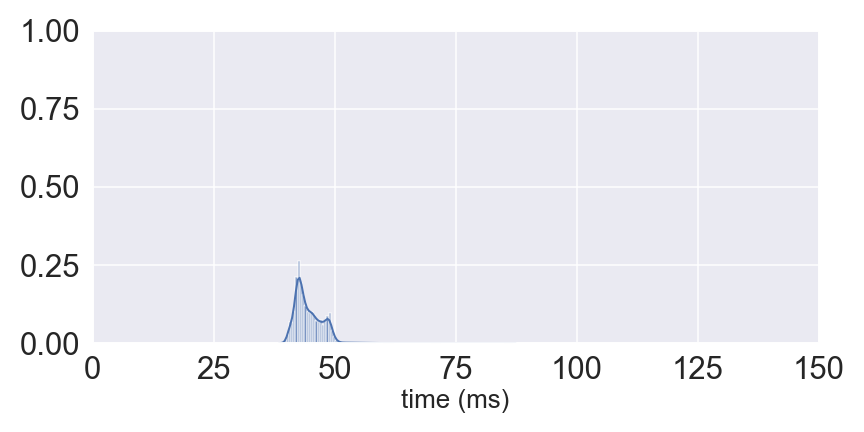
\includegraphics[width=\textwidth,height=.2\textheight,keepaspectratio]{figures/inference_plots/gpu_resnet_inference_time_distribution}}
		\hfill
		\subfloat[B-\gls{resnet}]{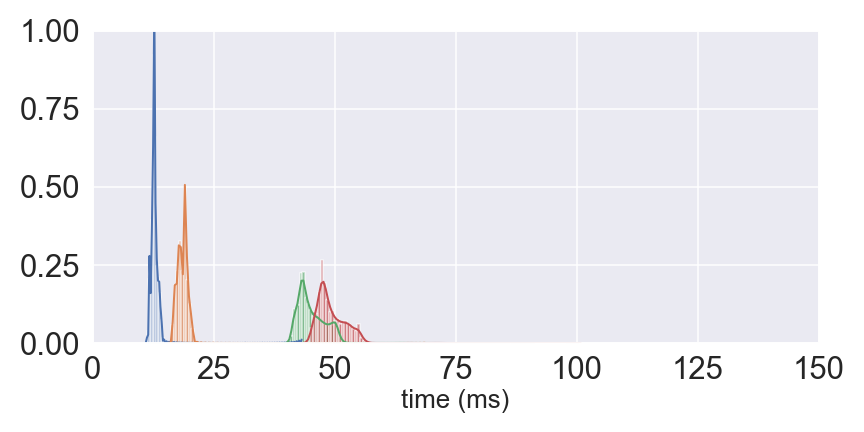
\includegraphics[width=\textwidth,height=.2\textheight,keepaspectratio]{figures/inference_plots/gpu_b-resnet_inference_time_distribution}}
		\hfill
		\subfloat[\gls{densenet} ]{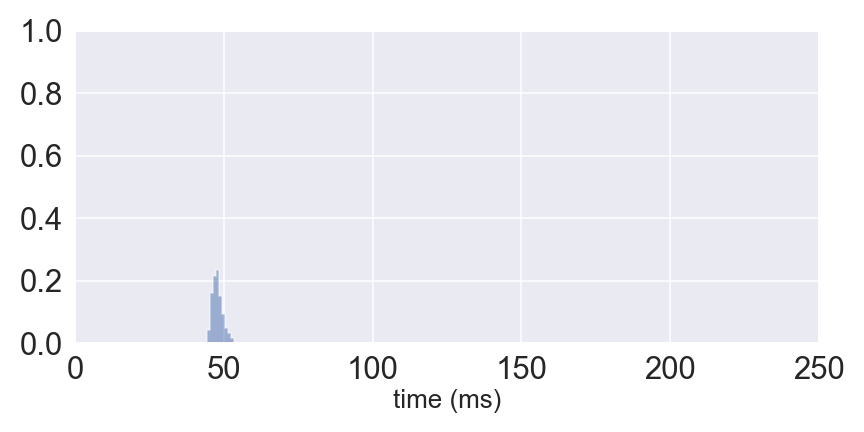
\includegraphics[width=\textwidth,height=.2\textheight,keepaspectratio]{figures/inference_plots/gpu_densenet_inference_time_distribution}}
		\hfill
		\subfloat[B-\gls{densenet}]{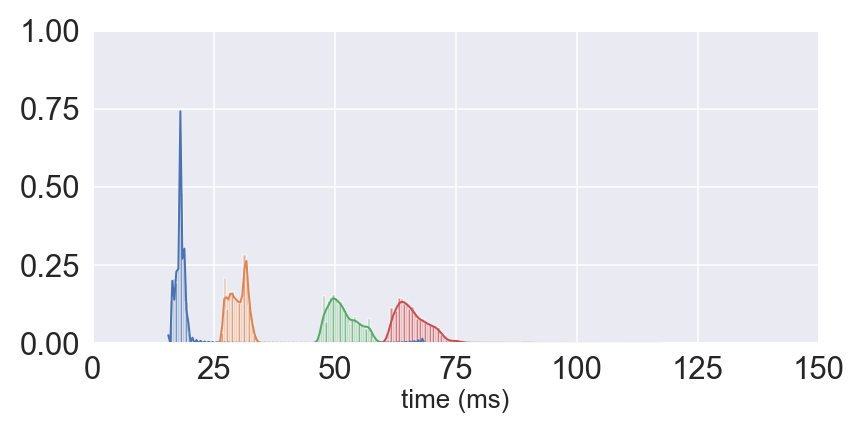
\includegraphics[width=\textwidth,height=.2\textheight,keepaspectratio]{figures/inference_plots/gpu_b-densenet_inference_time_distribution}}
		\hfill
		\subfloat[\gls{msdnet}]{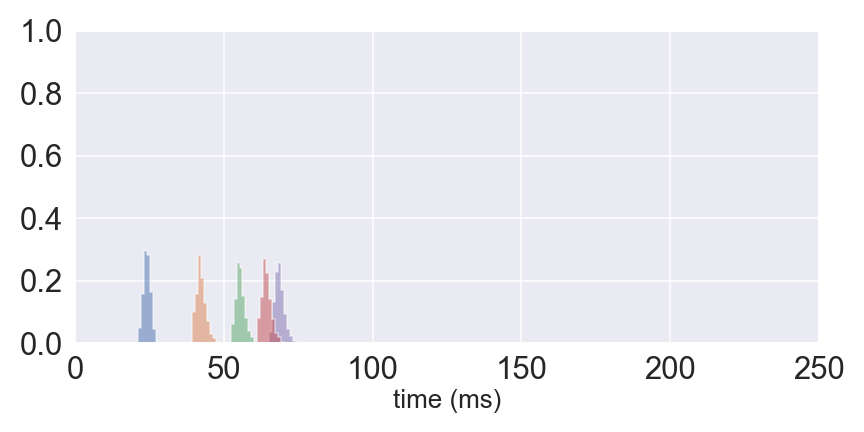
\includegraphics[width=\textwidth,height=.2\textheight,keepaspectratio]{figures/inference_plots/gpu_msdnet_inference_time_distribution}}
	\end{minipage}
	\begin{minipage}{0.33\textwidth}
		\captionsetup[subfigure]{farskip=0pt,captionskip=0pt,justification=centering}
		\centering
		Jetson TX2
		\subfloat[\gls{resnet} ]{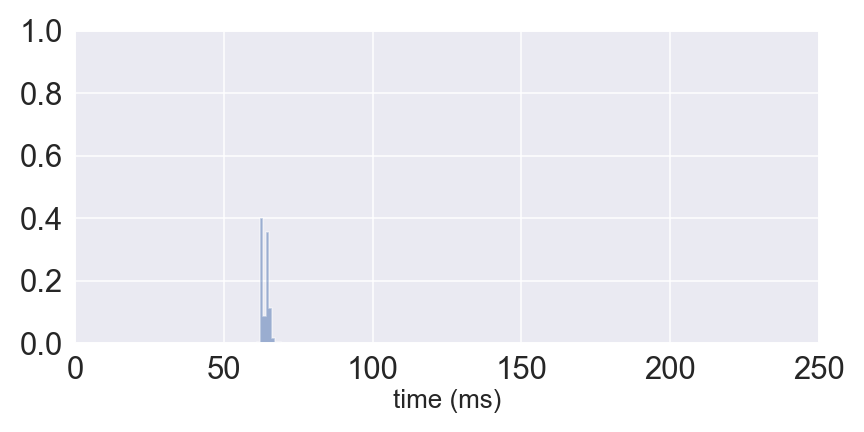
\includegraphics[width=\textwidth,height=.2\textheight,keepaspectratio]{figures/inference_plots/jetson_resnet_inference_time_distribution}}
		\hfill
		\subfloat[B-\gls{resnet}]{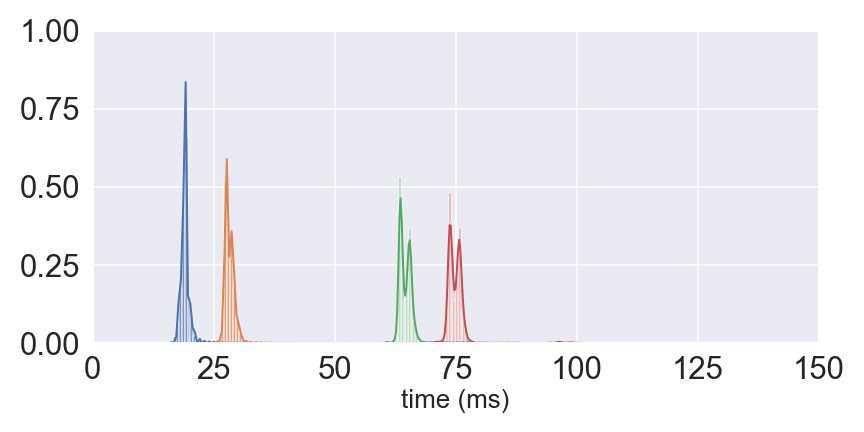
\includegraphics[width=\textwidth,height=.29\textheight,keepaspectratio]{figures/inference_plots/jetson_b-resnet_inference_time_distribution}}
		\hfill
		\subfloat[\gls{densenet} ]{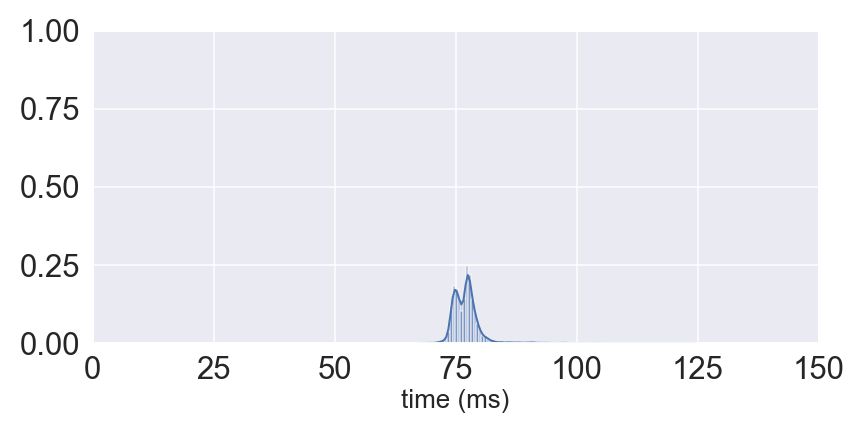
\includegraphics[width=\textwidth,height=.2\textheight,keepaspectratio]{figures/inference_plots/jetson_densenet_inference_time_distribution}}
		\hfill
		\subfloat[B-\gls{densenet}]{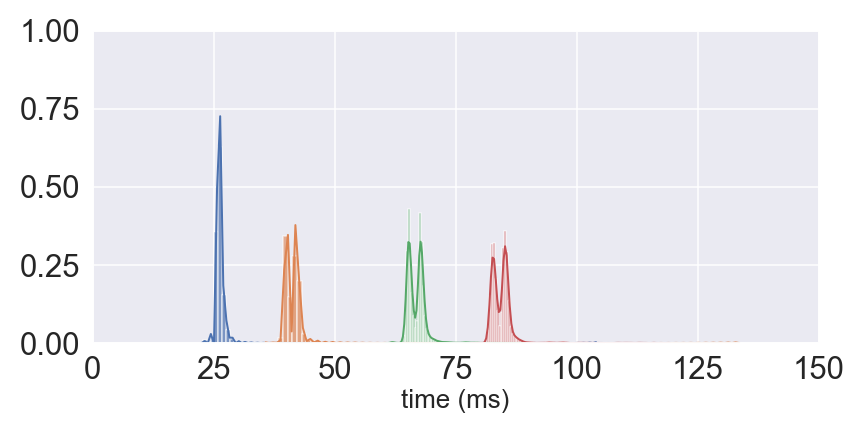
\includegraphics[width=\textwidth,height=.2\textheight,keepaspectratio]{figures/inference_plots/jetson_b-densenet_inference_time_distribution}}
		\hfill
		\subfloat[\gls{msdnet}]{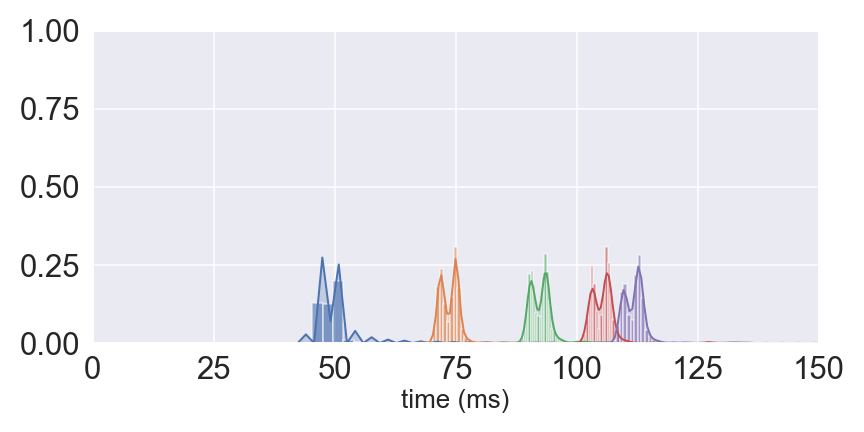
\includegraphics[width=\textwidth,height=.2\textheight,keepaspectratio]{figures/inference_plots/jetson_msdnet_inference_time_distribution}}
	\end{minipage}
	\begin{minipage}{.33\textwidth}
		\captionsetup[subfigure]{farskip=0pt,captionskip=0pt,justification=centering}
		\centering
		Intel NUC
		\subfloat[\gls{resnet} ]{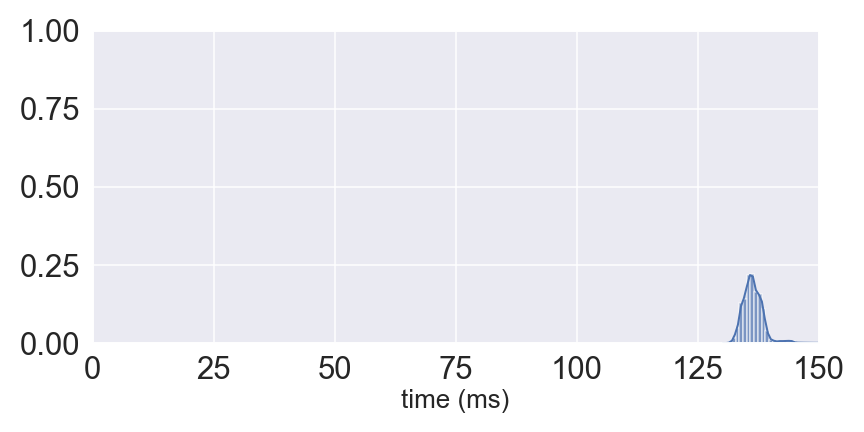
\includegraphics[width=\textwidth,keepaspectratio]{figures/inference_plots/nuc_resnet_inference_time_distribution}}
		\hfill
		\subfloat[B-\gls{resnet}]{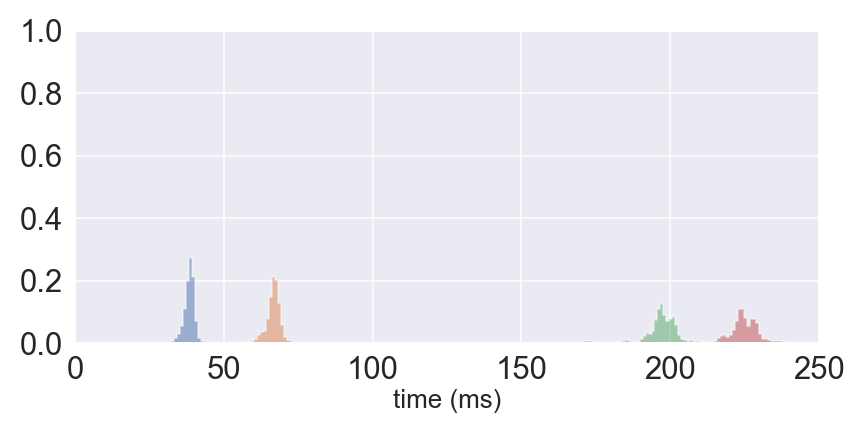
\includegraphics[width=\textwidth,height=.2\textheight,keepaspectratio]{figures/inference_plots/nuc_b-resnet_inference_time_distribution}}
		\hfill
		\subfloat[\gls{densenet} ]{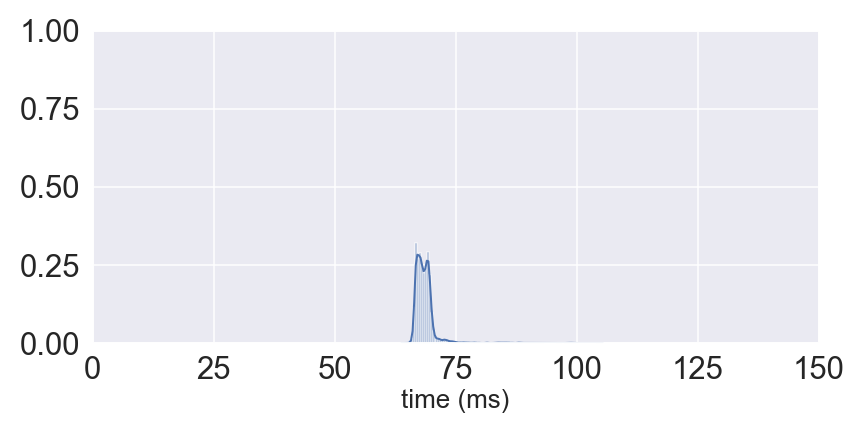
\includegraphics[width=\textwidth,keepaspectratio]{figures/inference_plots/nuc_densenet_inference_time_distribution}}
		\hfill
		\subfloat[B-\gls{densenet}]{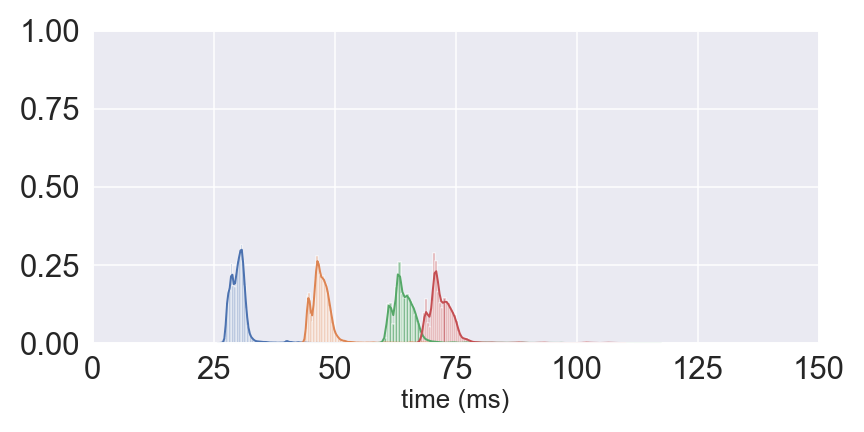
\includegraphics[width=\textwidth,keepaspectratio]{figures/inference_plots/nuc_b-densenet_inference_time_distribution}}
		\hfill
		\subfloat[\gls{msdnet}]{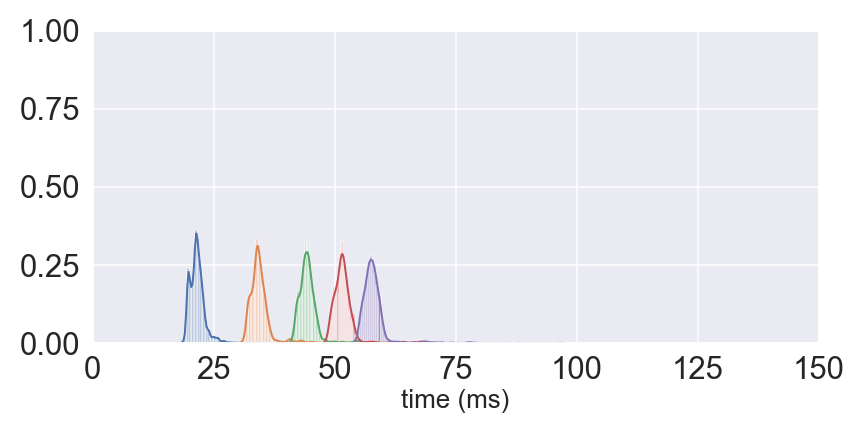
\includegraphics[width=\textwidth,keepaspectratio]{figures/inference_plots/nuc_msdnet_inference_time_distribution}}	
	\end{minipage}
	\caption[Platform Inference Time of \gls{dnn}s]{Inference Time Distribution, left column: GPU Workstation (a-e), center column: Jetson TX2 (f-j), right column NUC (k-o)}
	\label{fig:inference-time-dist}
\end{figure}

We have shown, that it is possible to achieve better runtimes using an early exit. In the next section we investigate how to allow samples to exit the model early using the score output from the softmax classfier, where we also experiment with our two different score function: score-max and score-margin.

\subsubsection{Theoretical Exit Score Threshold Analysis}

We mentioned in section \ref{sec:ee-branchy-vs-cascaded}, that a score threshold can be used to control the accuracy-latency trade-off of early exiting models. If too high threshold is selected only a few samples can confidently exit the model at an early exit, thus no significant delay improvements may be found. Contrary, if too low a threshold is selected a huge delay improvement may be found, however at a corresponding cost in accuracy. 

This analysis is theoretical, as the early exiting mechanism is in fact not exploited. All samples are allowed to pass all the way to the end of the network, thus all samples are classified at each exit. We log the predicted class label and score output. Using the two different score functions, $ f_{max} $ and $ f_{margin} $, we mark a sample exitable, if the output of the score function higher than the threshold. We analyse all models against a range of thresholds $ \gamma = \left\{0.1, 0.1, \dots 0,9\right\} $.

\Cref{fig:resnet_confidence,fig:resnet_score-margin,fig:densenet_confidence,fig:densenet_score-margin,fig:msdnet_confidence,fig:msdnet_score-margin} compares all exits of all early exit models a rising threshold. We plot the result for both score functions.
The figures shows the frequency of exited samples, that have been correctly classified and exited ({\color{sns-green}green}), and incorrectly classified and exited due to satisfying score ({\color{sns-red}red}). The frequency of not exited samples ({\color{sns-blue}blue}). The line plotted on each subfigure, shows the change in exiting accuracy, as we raise the confidence score requirements ({\color{sns-orange}orange}). By exiting accuracy we mean the ratio of correctly classified out of all exited samples, hence we do not care for not exited samples.

We want to reduces the amount of incorrectly exited samples ({\color{sns-red}red}). Whenever a sample is exited incorrectly, the overall accuracy of the model is reduced, if it could have been correctly classifed at later exit. The growing frequency of correctly exited samples ({\color{sns-green}green}) at later exits, exemplifies the improved accuracy at deeper exits in the models. Raising the threshold results in a higher exited accuracy, as the amount incorrectly exited is reduced more, than the number of correctly exited samples. 

Generally \emph{score-margin} has more desirable traits, as less samples are incorrectly exited ({\color{sns-red}red}), at the expense of additional samples not exited ({\color{sns-blue}blue}). The result matches \cite{park_big/little_2015,tann_flexible_2018}, showing a stronger correlation for the \emph{score-margin} and accuracy, than confidence score and accuracy. 

\newcounter{imagenumber}
\begin{center}
\begin{minipage}{\textwidth}
	\begin{figure}
		\centering
		\paragraph{B-ResNet}
		\includegraphics[width=\linewidth]{figures/threshold_plots/threshold_analysis_legend}
	\end{figure}
	
	\begin{minipage}{0.5\textwidth}
		\begin{figure}
			\captionsetup[subfloat]{farskip=1pt,captionskip=1pt, justification=centering}
			\centering
			\forloop{imagenumber}{0}{\value{imagenumber} < 4}{
				
				\subfloat[Exit-\arabic{imagenumber}\label{fig:confidence_resnet_exit_\arabic{imagenumber}}]{\includegraphics[width=.9\linewidth]{figures/threshold_plots/threshold_analysis_b-resnet_confidence_\arabic{imagenumber}}}
				\hfill
			}
			\caption[ResNet Confidence Threshold]{Confidence Threshold}
			\label{fig:resnet_confidence}
		\end{figure}
	\end{minipage}
\hfill
	\begin{minipage}{0.5\textwidth}
		\begin{figure}
			\captionsetup[subfloat]{farskip=1pt,captionskip=1pt, justification=centering}
			\centering
			\forloop{imagenumber}{0}{\value{imagenumber} < 4}{
				
				\subfloat[Exit-\arabic{imagenumber}\label{fig:score-margin_resnet_exit_\arabic{imagenumber}}]{\includegraphics[width=.9\linewidth]{figures/threshold_plots/threshold_analysis_b-resnet_score-margin_\arabic{imagenumber}}}
				\hfill
			}
			\caption[ResNet Score-margin Threshold]{Score-margin Threshold}
			\label{fig:resnet_score-margin}
		\end{figure}
	\end{minipage}
\end{minipage}
\end{center}


\begin{center}
\begin{minipage}{\textwidth}
	\begin{figure}
		\centering
		\paragraph{B-DenseNet}
	\end{figure}
	\begin{minipage}{0.5\textwidth}
		\begin{figure}
			\captionsetup[subfloat]{farskip=1pt,captionskip=1pt, justification=centering}
			\centering
			\forloop{imagenumber}{0}{\value{imagenumber} < 4}{
				
				\subfloat[Exit-\arabic{imagenumber}\label{fig:confidence_dense_exit_\arabic{imagenumber}}]{\includegraphics[width=.9\linewidth]{figures/threshold_plots/threshold_analysis_b-densenet_confidence_\arabic{imagenumber}}}
				\hfill
			}
			\caption[DenseNet Confidence Threshold]{Confidence Threshold}
			\label{fig:densenet_confidence}
		\end{figure}
	\end{minipage}
\hfill
	\begin{minipage}{0.5\textwidth}
		\begin{figure}
			\captionsetup[subfloat]{farskip=1pt,captionskip=1pt, justification=centering}
			\centering
			\forloop{imagenumber}{0}{\value{imagenumber} < 4}{
				
				\subfloat[Exit-\arabic{imagenumber}\label{fig:score-dense_resnet_exit_\arabic{imagenumber}}]{\includegraphics[width=.9\linewidth]{figures/threshold_plots/threshold_analysis_b-densenet_score-margin_\arabic{imagenumber}}}
				\hfill
			}
			\caption[DenseNet Score-margin Threshold]{Score-margin Threshold}
			\label{fig:densenet_score-margin}
		\end{figure}
	\end{minipage}
\end{minipage}
\end{center}


\noindent\makebox[\textwidth][c]{\begin{minipage}{0.9\textwidth}
		\begingroup
		\leftskip=0cm plus 0.5fil \rightskip=0cm plus -0.5fil
		\parfillskip=0cm plus 1fil
		\paragraph{MSDNet}\par
		\endgroup
		
		\begin{minipage}{0.5\textwidth}
			\begin{figure}
				\captionsetup[subfloat]{farskip=0pt,captionskip=0pt, justification=centering}
				\centering
				\forloop{imagenumber}{0}{\value{imagenumber} < 5}{
					
					\subfloat[Exit-\arabic{imagenumber}\label{fig:confidence_msd_exit_\arabic{imagenumber}}]{\includegraphics[width=.9\linewidth]{figures/threshold_plots/threshold_analysis_msdnet_confidence_\arabic{imagenumber}}}
					\hfill
				}
				\caption[MSDNet Confidence Threshold]{Confidence Threshold}
				\label{fig:msdnet_confidence}
			\end{figure}
		\end{minipage}
	\hfill
		\begin{minipage}{0.5\textwidth}
			\begin{figure}
				\captionsetup[subfloat]{farskip=1pt,captionskip=1pt, justification=centering}
				\centering
				\forloop{imagenumber}{0}{\value{imagenumber} < 5}{
					
					\subfloat[Exit-\arabic{imagenumber}\label{fig:score-msdnet_exit_\arabic{imagenumber}}]{\includegraphics[width=.9\linewidth]{figures/threshold_plots/threshold_analysis_msdnet_score-margin_\arabic{imagenumber}}}
					\hfill
				}
				\caption[MSDNet Score-margin Threshold]{Score-margin Threshold}
				\label{fig:msdnet_score-margin}
			\end{figure}
		\end{minipage}
\end{minipage}}

\subsubsection{Practical Exit Score Threshold Analysis}

We want to evaluate early exiting capabilities in practice. We exploit the exit mechanism to terminate inference, if a satisfying score is obtained. If a samples reaches the last exit, it is classified irregardless of threshold being passed or not. Figure \ref{fig:model_c-threshold_comparison} presents the result using the score-max and figure \ref{fig:model_threshold_comparison} using the score-margin.

\begin{minipage}{\linewidth}
	\begin{figure}
		\captionsetup[subfloat]{justification=centering, captionskip=0pt, farskip=0pt}
		\centering
		\includegraphics[width=.5\linewidth]{figures/inference_plots/model_bar_legend}
	\end{figure}
	\begin{figure}
		\captionsetup[subfloat]{justification=centering, captionskip=0pt, farskip=1pt}
		\centering
		\subfloat[$T= 0.1$\label{fig:model-c-threshold_comparison_t_1}]{\includegraphics[width=.33\linewidth]{figures/inference_plots/model_confidence_comparison_1}}
		\hfill
		\subfloat[$T= 0.2$\label{fig:model-c-threshold_comparison_t_2}]{\includegraphics[width=.33\linewidth]{figures/inference_plots/model_confidence_comparison_2}}
		\hfill
		\subfloat[$T= 0.3$\label{fig:model-c-threshold_comparison_t_3}]{\includegraphics[width=.33\linewidth]{figures/inference_plots/model_confidence_comparison_3}}
		\hfill
		\subfloat[$T= 0.4$\label{fig:model-c-threshold_comparison_t_4}]{\includegraphics[width=.33\linewidth]{figures/inference_plots/model_confidence_comparison_4}}
		\hfill
		\subfloat[$T= 0.5$\label{fig:model-c-threshold_comparison_t_5}]{\includegraphics[width=.33\linewidth]{figures/inference_plots/model_confidence_comparison_5}}
		\hfill
		\subfloat[$T= 0.6$\label{fig:model-c-threshold_comparison_t_6}]{\includegraphics[width=.33\linewidth]{figures/inference_plots/model_confidence_comparison_6}}
		\hfill
		\subfloat[$T= 0.7$\label{fig:model-c-threshold_comparison_t_7}]{\includegraphics[width=.33\linewidth]{figures/inference_plots/model_confidence_comparison_7}}
		\hfill
		\subfloat[$T= 0.8$\label{fig:model-c-threshold_comparison_t_8}]{\includegraphics[width=.33\linewidth]{figures/inference_plots/model_confidence_comparison_8}}
		\hfill
		\subfloat[$T= 0.9$\label{fig:model-c-threshold_comparison_t_9}]{\includegraphics[width=.33\linewidth]{figures/inference_plots/model_confidence_comparison_9}}
		
		\caption[Model comparison of early exit capabilities using confidence threshold]{Model comparison of early exit capabilities using score-max}
		\label{fig:model_c-threshold_comparison}
	\end{figure}

\todo{T is now gamma...}
	
\end{minipage}

\begin{minipage}{\linewidth}
	\begin{figure}
		\captionsetup[subfloat]{justification=centering, captionskip=0pt, farskip=0pt}
		\centering
		\includegraphics[width=.5\linewidth]{figures/inference_plots/model_bar_legend}
	\end{figure}
	\begin{figure}
		\captionsetup[subfloat]{justification=centering, captionskip=0pt, farskip=1pt}
		\centering
		\subfloat[$T= 0.1$\label{fig:model-threshold_comparison_t_1}]{\includegraphics[width=.33\linewidth]{figures/inference_plots/model_comparison_1}}
		\hfill
		\subfloat[$T= 0.2$\label{fig:model-threshold_comparison_t_2}]{\includegraphics[width=.33\linewidth]{figures/inference_plots/model_comparison_2}}
		\hfill
		\subfloat[$T= 0.3$\label{fig:model-threshold_comparison_t_3}]{\includegraphics[width=.33\linewidth]{figures/inference_plots/model_comparison_3}}
		\hfill
		\subfloat[$T= 0.4$\label{fig:model-threshold_comparison_t_4}]{\includegraphics[width=.33\linewidth]{figures/inference_plots/model_comparison_4}}
		\hfill
		\subfloat[$T= 0.5$\label{fig:model-threshold_comparison_t_5}]{\includegraphics[width=.33\linewidth]{figures/inference_plots/model_comparison_5}}
		\hfill
		\subfloat[$T= 0.6$\label{fig:model-threshold_comparison_t_6}]{\includegraphics[width=.33\linewidth]{figures/inference_plots/model_comparison_6}}
		\hfill
		\subfloat[$T= 0.7$\label{fig:model-threshold_comparison_t_7}]{\includegraphics[width=.33\linewidth]{figures/inference_plots/model_comparison_7}}
		\hfill
		\subfloat[$T= 0.8$\label{fig:model-threshold_comparison_t_8}]{\includegraphics[width=.33\linewidth]{figures/inference_plots/model_comparison_8}}
		\hfill
		\subfloat[$T= 0.9$\label{fig:model-threshold_comparison_t_9}]{\includegraphics[width=.33\linewidth]{figures/inference_plots/model_comparison_9}}
		
		\caption[Model comparison of early exit capabilities]{Model comparison of early exit capabilities using score-margin}
		\label{fig:model_threshold_comparison}
	\end{figure}
	
\end{minipage}

The subfigures of figure \ref{fig:model_c-threshold_comparison} and \ref{fig:model_threshold_comparison} show the raised score requirements. Each subfigure presents a subplot of the frequency of correctly exited samples and a subplot of incorrectly exit samples at each exit for all three models. For each model the bars sum to one across the subplots, which is equivalent to all samples of the test. Note, that only a few samples actually require the last exits. Especially at low thresholds the last exit is almost never used. It looks like we move all bars more to the right, as the threshold is raised, i.e. forcing the model to use later exits and less samples are incorrect classified. \gls{bdensenet} and especially \gls{msdnet}, can more frequently exit samples at earliest exits even at high thresholds values, whereas \gls{bresnet} put significantly more weight on its second last exit. 

This result clearly indicates, that we can in fact reduce the average inference delay by using the exit condition. In the next section we evaluate the score threshold's impact on the accuracy-latency trade-off.

\subsubsection{Score Threshold and the Accuracy-Latency Trade-Off}

Figure \ref{fig:threshold-acc-lat-trade-off} show the inference accuracy and latency of all the models, on the platforms. 

\begin{figure}
	\captionsetup[subfigure]{justification=centering,farskip=0pt,captionskip=0pt}
	\centering
	\includegraphics[width=.4\linewidth]{figures/threshold_plots/inference_legend}
	\subfloat[GPU Workstation\label{fig:early_exit_vs_conv}]{\includegraphics[width=\textwidth,height=.22\textheight,keepaspectratio]{figures/threshold_plots/gpu_inference}}
	\hfill
	\subfloat[Jetson TX2\label{fig:jetson-early_exit_vs_conv}]{\includegraphics[width=\textwidth,height=.22\textheight,keepaspectratio]{figures/threshold_plots/jetson_inference}}
	\hfill
	\subfloat[NUC\label{fig:nuc-early_exit_vs_conv}]{\includegraphics[width=\textwidth,height=.22\textheight,keepaspectratio]{figures/threshold_plots/nuc_inference}}
	\caption[Threshold Accuracy-Latency Trade-off]{Threshold Accuracy-Latency Trade-off on \protect\subref{fig:early_exit_vs_conv} GPU Workstation, \protect\subref{fig:jetson-early_exit_vs_conv} Jetson TX2 and \protect\subref{fig:nuc-early_exit_vs_conv} NUC }
	\label{fig:threshold-acc-lat-trade-off}
\end{figure}

Irregardless of platform, the results clearly exemplifies the accuracy-latency trade-off imposed by the early exit model. Raising the score threshold improves the models' accuracy. However, also introduces more latency. As we saw in the previous section, raising the score threshold, forces the model to use later exits more frequently to reach a satisfying score. 

In figure \ref{fig:threshold-acc-lat-trade-off-by-time} \ref{fig:threshold-acc-lat-trade-off}, we plotting the accuracy against the mean time.
\begin{figure}
	\captionsetup[subfigure]{justification=centering,farskip=0pt,captionskip=0pt}
	\centering
	\includegraphics[width=.4\linewidth]{figures/threshold_plots/inference_by_time_legend}
	\subfloat[GPU Workstation\label{fig:gpu-early_exit_vs_time}]{\includegraphics[width=\textwidth,height=.22\textheight,keepaspectratio]{figures/threshold_plots/gpu_inference_by_time}}
	\hfill
	\subfloat[Jetson TX2\label{fig:jetson-early_exit_vs_time}]{\includegraphics[width=\textwidth,height=.22\textheight,keepaspectratio]{figures/threshold_plots/jetson_inference_by_time}}
	\hfill
	\subfloat[NUC\label{fig:nuc-early_exit_vs_time}]{\includegraphics[width=\textwidth,height=.22\textheight,keepaspectratio]{figures/threshold_plots/nuc_inference_by_time}}
	\caption[Threshold Accuracy-Latency Trade-off]{Threshold Accuracy-Latency Trade-off on \protect\subref{fig:early_exit_vs_conv} GPU Workstation, \protect\subref{fig:jetson-early_exit_vs_conv} Jetson TX2 and \protect\subref{fig:nuc-early_exit_vs_conv} NUC }
	\label{fig:threshold-acc-lat-trade-off-by-time}
\end{figure}

Clearly the model becomes more accurate when having more time. The conventional models achieve a higher accuracy, however also requires more time, than their more flexible early exiting counterpart.

In most circumstances the \gls{bresnet} is the fastest on most accurate model on the \gls{gpu}-workstation and the Jetson. On the NUC, we can see \gls{bresnet}, is drastically slower, where \gls{msdnet} is outstandingly the best model. In table \ref{tbl:score-acc-lat-trade} we present the change in accuracy and time using different threshold compared to letting the end exit of the early exit model classify the sample.

\begin{minipage}[t]{\linewidth}\begin{small}
	
	\begin{longtabu}{>{\bfseries}X|X|X[r]|X[r]|X[r]|X[r]}
		\caption[Score Threshold Accuracy-Latency Trade-off]{Score Threshold Accuracy-Latency Trade-off}\label{tbl:score-acc-lat-trade} \\
		\toprule
		\rowfont{\bfseries}
		& & & {GPU Workstation} &  {Jetson TX2} & {Intel NUC} \tabularnewline
		\rowfont{\bfseries} Model & Threshold & Acc. dif. & Time dif.  & Time dif. & Time dif. \tabularnewline
		\hline
		\endfirsthead
		\multicolumn{3}{@{}l}{\textbf{\textcolor{black}{Table \ref{tbl:score-acc-lat-trade}:}} continued}\\
		\toprule
		\rowfont{\bfseries}
		& &  & {GPU Workstation} &  {Jetson TX2} & {Intel NUC} \tabularnewline
		\rowfont{\bfseries} Model & Threshold & Acc. dif. & Time dif.  & Time dif. & Time dif. \tabularnewline
		\hline
		\endhead % all the lines above this will be repeated on every page
		\hline
		\multicolumn{3}{@{}l}{continued \ldots}\\
		\endfoot
		\hline
		\multirow{11}{*}{B-ResNet} & End (No Exit) & 0.88 & 37.14 & 67.04 & 223.32  \tabularnewline \tabucline{2-7}
		& $ \gamma = 0.1 $ 	& -0.24 & -19.76 & -40.87 & -181.53 \tabularnewline
		&$ \gamma = 0.2 $ 	& -0.15 & -16.10 & -36.11 & -171.44 \tabularnewline 
		&$ \gamma = 0.3 $ 	& -0.09 & -13.45 & -32.16 & -163.55 \tabularnewline
		&$ \gamma = 0.4 $ 	& -0.06 & -10.91 & -28.63 & -155.14 \tabularnewline 
		&$ \gamma = 0.5 $ 	& -0.03 &  -8.93 & -25.72 & -150.43 \tabularnewline
		&$ \gamma = 0.6 $ 	& -0.02 &  -7.20 & -23.01 & -144.25 \tabularnewline 
		&$ \gamma = 0.7 $ 	& -0.01 &  -5.09 & -20.16 & -141.93 \tabularnewline 
		&$ \gamma = 0.8 $ 	&  0.00 &  -3.39 & -17.34 & -136.39 \tabularnewline 
		&$ \gamma = 0.9 $ 	&  0.01 &  -0.40 & -13.24 & -127.15 \tabularnewline 
		\hline
		\multirow{11}{*}{B-DenseNet} & End (No Exit) & 0.87 & 49.14 & 72.40 & 72.21 \tabularnewline \tabucline{2-7}
		&$ \gamma = 0.1 $ 	& -0.21 & -27.08 & -40.33 & -36.65  \tabularnewline
		&$ \gamma = 0.2 $ 	& -0.14 & -24.04 & -37.60 & -33.54  \tabularnewline 
		&$ \gamma = 0.3 $ 	& -0.10 & -21.37 & -34.29 & -31.35  \tabularnewline
		&$ \gamma = 0.4 $ 	& -0.07 & -19.02 & -31.41 & -27.30  \tabularnewline 
		&$ \gamma = 0.5 $ 	& -0.04 & -16.94 & -28.77 & -25.00  \tabularnewline
		&$ \gamma = 0.6 $ 	& -0.03 & -14.57 & -26.07 & -25.17  \tabularnewline 
		&$ \gamma = 0.7 $ 	& -0.01 & -12.70 & -23.90 & -22.67  \tabularnewline 
		&$ \gamma = 0.8 $ 	&  0.00 & -10.32 & -20.95 & -18.66  \tabularnewline 
		&$ \gamma = 0.9 $ 	&  0.01 &  -6.94 & -17.07 & -17.85  \tabularnewline 
		\hline
		\multirow{11}{*}{MSDNet} & End (No Exit) & 0.86 & 68.87 & 103.29 & 56.02 \tabularnewline \tabucline{2-7}
		&$ \gamma = 0.1 $ 	& -0.09 & -29.52 & -51.30 & -33.14 \tabularnewline
		&$ \gamma = 0.2 $ 	& -0.08 & -28.15 & -50.39 & -32.45 \tabularnewline 
		&$ \gamma = 0.3 $ 	& -0.06 & -26.83 & -48.53 & -31.61 \tabularnewline
		&$ \gamma = 0.4 $ 	& -0.05 & -25.31 & -47.06 & -30.93 \tabularnewline 
		&$ \gamma = 0.5 $ 	& -0.04 & -23.95 & -45.31 & -29.81 \tabularnewline
		&$ \gamma = 0.6 $ 	& -0.03 & -22.32 & -43.40 & -28.86 \tabularnewline 
		&$ \gamma = 0.7 $ 	& -0.02 & -20.28 & -41.39 & -27.38 \tabularnewline 
		&$ \gamma = 0.8 $ 	& -0.01 & -17.79 & -38.73 & -25.88 \tabularnewline 
		&$ \gamma = 0.9 $ 	& -0.00 & -14.32 & -34.46 & -23.44 \tabularnewline 
		\bottomrule
	\end{longtabu}
\end{small}
\end{minipage}

From the table \ref{tbl:score-acc-lat-trade} we can tell, that selecting a high threshold introcuces only a small cost in accuracy, and for the most part, we can achieve significant time savings opposed to inferencing all the way to the last exit of the early exit models. Quite interesting we can actually see a minor improvement in accuracy using a threshold value of 0.9 for both \gls{resnet} and \gls{densenet}. Thus, some overthinking is mitigated selecting a high threshold.


We have shown, that early exit model can be used to reduce the latency with a compromise in accuracy, adjusted by a score threshold. The question, that remains is still, can we use early exits to meet delay requirement for time-critical application. 

\newpage\subsubsection{Reliability vs. Computation Latency}

As stated in our problem formulation, we want to maximize the reliability. Recall the reliability is the achieved accuracy achieved before a timeout. Everything that could not meet the deadline is missed and have a negative impact on the reliability.

\begin{figure}
	\captionsetup[subfigure]{justification=centering, farskip=0pt,captionskip=0pt}
	\centering
	\includegraphics[height=.05\textheight]{figures/delay_plots/delay_threshold_legend}
	\hfill
	\subfloat[GPU Workstation]{\includegraphics[width=\textwidth,height=.22\textheight,keepaspectratio]{figures/delay_plots/gpu__delay_threshold}}
	\hfill
	\subfloat[Jetson TX2]{\includegraphics[width=\textwidth,height=.22\textheight,keepaspectratio]{figures/delay_plots/jetson__delay_threshold}}
	\hfill
	\subfloat[NUC]{\includegraphics[width=\textwidth,height=.22\textheight,keepaspectratio]{figures/delay_plots/nuc__delay_threshold}}
	\caption[Reliability vs. Computation Latency]{Reliability vs. Delay Threshold}
	\label{fig:delay-threshold}
\end{figure}

We measured the time for a samples to reach a prediction at all exits. We analysed the accuracy given different deadlines with 1 ms granularity. In figure \ref{fig:delay-threshold}, we plot the reliability against increasing delay thresholds.

The result show staircase-like functions of reliability as we relax the delay constraint, which increases the reliability when more time ia available. The steps of the functions are loacted close to the mean time-to-prediction for a later exit of the model, see table \ref{tbl:inference-stats}. The dashed lines show the conventional model, clearly under very stringent delay requirement, we are able to improve the reliability using early exit models. However, if the last exit of the early exit model is always reachable, then the conventional models will achieve superior reliability. 

\section{Summary} \label{sec:ee-summary}

In summary of this chapter; we review early exiting literature and compare inference and training proposals. We formalize an analytical model to evaluate early exiting and conventional models. 

We have implemented \gls{bresnet} and \gls{bdensenet}. The early exits were placed after down-sampling layers or block, with the primary reason to reduce the offloading data size of intermediate features for collaborative edge. Even though we ended up not pursuing collaborative architectures, reasons why will be discussed later. We achieved satisfying early exit accuracy. However, in other works, such as \cite{huang_multi-scale_2017}, the placement of early exit is placed within the resolution- and dense blocks for repectively \gls{bresnet} and \gls{bdensenet}. However, they construct other versions of the \gls{bresnet} and \gls{bdensenet}, which have evenly distributed number of layers within each block, to evenly distribute the exits. Due to time constraints, we did not train from scratch, and wanted to apply and validate the \gls{branchynet} framework on existing architectures. Therefore we did not construct new versions of \gls{resnet} and \gls{densenet} with the number of layers. More importantly, in order not to slow the interference process, we limited ourselves to only 4 early exits classifiers. In fact \cite{berestizshevsky_sacrificing_2019} uses the same placement of classifiers, as in ours. For the same reasons; to limit the overhead and reduce wasted computation, we did not add convolution layers in exit branches as in \cite{teerapittayanon_branchynet:_2016}. Our exit only consists of a pooling layer to reduce the feature size and a linear classifier, as in \cite{kaya_shallow-deep_nodate}. 

We have successfully trained three early exiting models on the \gls{min100} dataset. We have shown, that freezing the model base as proposed in \cite{leroux_resource-constrained_2015}, did not allow for features to be optimized classifiers at early exits. Training the entire model, proposed in \cite{teerapittayanon_branchynet:_2016}, on the other hand did show satisfying validation accuracy. The \gls{msdnet} is able to obtain the highest accuracy of the early exit models, but \gls{bresnet} is able to obtain higher accuracy at the final exit. 

We measured inference time on three hardware platforms, which gave conflicting results. The inference timings have shown to be very dependent on the hardware characteristics. The GPU Workstation are enabled with the strongest \gls{gpu}, thus have the most parallelization capabilities and able to run especially \gls{resnet} faster, as this is more suited for \gls{gpu} parallelization \cite{lee_energy_2019}. However, \gls{densenet} and \gls{msdnet} has much lower amount of parameter and require less \gls{flop}s, hence would be expected to run faster. 

In \cite{lee_energy_2019} it is found, that \gls{densenet}'s linearly increasing amount of filters by continuous concatenation is inefficient on \gls{gpu}s, due to expensive memory accessing on \gls{gpu}s. They propose a new design, that still preserve information by concatenation. Instead they only concatenate once at the end of a block, thereby achieving runtime superior to \gls{densenet} and even comparable runtime and accuracy to \gls{resnet}. They question, if deep and thin networks are inefficient on \gls{gpu}s and argue, that \gls{flop}s alone is not a good measure of speed, when it comes to \gls{gpu} efficiency, and propose \gls{flop}s/s. Wide-Residual Networks are proposed in \cite{zagoruyko_wide_2017} as a more computational efficient version of \gls{resnet}, by taking advantage of larger tensors allow for more parallelization. 

The Intel NUC, shows the opposite trend, in fact the \gls{msdnet} outperform the other models, as it requires far fewer \gls{flop}s and are comprised of far fewer layers and parameters. The \gls{cpu}-only NUC cannot achieve the same level of parallelization to accelerate model inference. The \gls{msdnet} \cite{huang_multi-scale_2017} show very interestingly very good early exit accuracy. The model requires far less computation, than the \gls{bresnet} and \gls{bdensenet}. It has surprisingly good inference time on the \gls{nuc}. However, it halts on the \gls{gpu}-enabled platforms. The \gls{bresnet} achieve decent runtimes utilizing a \gls{gpu}, whereas \gls{bdensenet} achieve decent runtime in either case.Research in parallelization and operation is important to come of with even better models, that works across platforms.

We investigated score threshold as a mechanism to exit samples early. We used both score-max and score-margin. The max score confidence threshold is widely used in early exiting literature \cite{leroux_resource-constrained_2015, leroux_cascading_2017, kaya_shallow-deep_nodate, berestizshevsky_sacrificing_2019}. The score-margin has not been used directly for early exiting, but used in model selection frameworks \cite{park_big/little_2015,tann_flexible_2018}. The score-margin was able to remove most incorrectly exited samples, when choosing a sufficiently high threshold value. However, it was also at the cost of some samples, that could have exited correctly, now not able to be exited. Additionally we compared the early exiting capabilities of the models. The model comprised of densely connected blocks \gls{bdensenet} and \gls{msdnet}, was able to correctly exit more sample at early exits, where the model designed for early exiting, \gls{msdnet} outperformed its competitors. We also studied the accuracy-latency trade-off, by letting samples exit the model at early exits. Early exit models can indeed save time compared with the conventional models, especially when selecting a low threshold value. We compared the models by plotting the accuracy by time, the \gls{bresnet} was found out to be the best model at making a compromise between accuracy and latency on the \gls{gpu}-enabled platforms. In sharp contrast to the \gls{cpu} of the NUC, where both the \gls{bdensenet} and \gls{msdnet} were better.

Finally, we evaluated the obtainable reliability by a delay threshold. The conventional models are outperformed at stringent delay threshold. \gls{bresnet} is still the better on the \gls{gpu}-enabled platforms. However, not as exclusively as figure \ref{fig:threshold-acc-lat-trade-off-by-time} shows. At certain delay threshold \gls{bdensenet} is actually better. 

Figure \ref{fig:delay-threshold} encourages model selection, where the most reliable model is chosen based on the required delay threshold. All analyses have led us to our inference scheme suitable for on-device, edge offloading and collaborative inference. In the next chapter we present this scheme, and show it is able to improve the reliability of time-critical applications at the edge.